\documentclass[conference]{IEEEtran}
\IEEEoverridecommandlockouts
% The preceding line is only needed to identify funding in the first footnote. If that is unneeded, please comment it out.
\usepackage{cite}
\usepackage{xurl}
\usepackage{amsmath,amssymb,amsfonts}
\usepackage{algorithmic}
\usepackage{graphicx}
\usepackage{textcomp}
\usepackage{xcolor}
\usepackage{cleveref, array, booktabs, threeparttable}
\usepackage{kotex}
\usepackage{makecell}
\usepackage{float}
\usepackage{subcaption}
\usepackage{tabularx}
\usepackage{longtable}
\usepackage{multicol}
\usepackage{listings}
\usepackage{cleveref, array, booktabs, threeparttable}
\usepackage{tabu} 
\usepackage{enumitem}
\usepackage{blindtext}
\usepackage[english]{babel}
\usepackage{comment}

\usepackage[export]{adjustbox}
\def\BibTeX{{\rm B\kern-.05em{\sc i\kern-.025em b}\kern-.08em
    T\kern-.1667em\lower.7ex\hbox{E}\kern-.125emX}}
\usepackage{graphicx}
\graphicspath{ {image/}{page/} }

\begin{document}

\title{DANBI – My Home’s Water Secretary\\
{\footnotesize \textsuperscript{*}Team Name : LeGend}

}

\author{\IEEEauthorblockN{Kim Eunho}
\IEEEauthorblockA{\textit{dept. Information System} \\
\textit{Hanyang Univ.}\\
Seoul, Republic of Korea \\
applejam5@naver.com}
\and
\IEEEauthorblockN{Oh Jiyun}
\IEEEauthorblockA{\textit{dept. Information System} \\
\textit{Hanyang Univ.}\\
Seoul, Republic of Korea \\
baram0516@naver.com}
\and
\IEEEauthorblockN{Jeong Hyoeun}
\IEEEauthorblockA{\textit{dept. Information System} \\
\textit{Hanyang Univ.}\\
Seoul, Republic of Korea \\
gydms415@hanyang.ac.kr}
\and
\IEEEauthorblockN{Choi Soojung}
\IEEEauthorblockA{\textit{dept. Information System} \\
\textit{Hanyang Univ.}\\
Seoul, Republic of Korea \\
tnwjd5127@naver.com}

}

\maketitle

\begin{abstract}
Now that humans, pets, and plants all live in a family, there are many things to care about and it is becoming difficult to manage them at once. We developed 'DANBI' that intuitively manages water intake information of all members of our family at once focusing on water, which is the basis of all life. DANBI is our water secretary which informs us when necessary with convenience through technical linkage with LG PuriCare water purifiers and NUGU speakers.
\end{abstract}

\begin{IEEEkeywords}
water secretary for family, water intake managing application, LG PuriCare water purifier, NUGU, and etc.
\end{IEEEkeywords}

\ 

\begin{table}[ht!] \renewcommand\arraystretch{1.25}
  \begin{threeparttable}
      \caption{Role Assignments%
      \label{tab:table1}}    %% Caption above tabular, label inside caption
      \begin{tabular}{@{}l l>{\raggedright\arraybackslash}p{3.8cm}@{}}
      \toprule
      \bfseries Role & \bfseries Name & \multicolumn{1}{l}{\bfseries Task description and etc.} \\
      \midrule
      User & Oh Jiyun & Think of ideas and design functions to improve usability. Specify people's need and suggest how to implement it as service functions. \\
      Customer & Jeong Hyoeun & Examine the service of the competitors and plan functions that could be our differentiator from others. Consider UI design which can attract the customers. \\
      Software developer & Choi Soojung & Be responsible for software development. Understanding user needs, developing software solutions, monitoring performance and modifying programs as needed. \\
      Development manager & Kim Eunho & Make a plan in order and quarterly to achieve the project's goals. Assign team members to their own roles and continuously check the progress of the work. \\
      \bottomrule
      \end{tabular}
  \end{threeparttable}
\end{table}

\ 

\section{Introduction}

\subsection{Motivation}\label{AA}
\setlength{\parindent}{2ex}
Water is the most fundamental factor in maintaining a person's life. Drinking insufficient water increases the risk of exposure to various diseases such as kidney stones, obesity, diabetes, bladder cancer, and colon cancer. Nevertheless, the proportion of 'people who intake sufficient water' decreases every year, and 6 out of 10 people are reported not to have enough water. Therefore, there is a need for a service that properly helps with water intake, and we developed this service using applications and AI speakers.

At the same time, this service allows you to manage the water supply of pets and plants together. In modern society, the form of family is changing. More and more people live with pets and plants, and unlike before, they begin to regard them as family members. As a result, people became more interested in their health care. For pets and plants, water intake is directly related to maintenance of life. In the case of pets, insufficient water intake can lead to diseases. Typically, it damages the kidneys and pancreas, which leads to renal failure and pancreatitis. For plant, water is a carrier of nutrients, which extracts nutrients from the soil and transports them to the end of the plant's leaves. Without enough water in cells, plants become malnourished and unable to support their own weight. Therefore, we created DANBI that helps manage water intake of humans, pets, and plants, that is, all of our family.

DANBI is a pure Korean word that means rain that falls appropriately when necessary. Like rain that falls when necessary on dry land, it means that it helps humans, pets, and plants drink proper water through notifications in busy modern society.

\ 
\subsection{Problem Statement}
\setlength{\parindent}{2ex}
People fully understand that all creatures have to take water enough. However, do you know how much water do you drink daily? Probably, most of people would not be able to figure out the amount of water they intake. Besides, the interval of drinking water is also important as the quantity of water people drink. But drinking water regularly is not easy for busy modern people. This is same for taking care of water intake of pets and plants which are part of our life. Therefore, the function which records water intake of people, pets and plants at our home, and sends notifications periodically will be a great help for us. Of course, there are several mobile applications providing service like this, but they have some inconvenient problems.

To use mobile applications which manage water intake of people or pets, the users have to write the amount of water they drink in person everyday. This way is very annoying since the users have difficulty to know exact quantity of water they intake. However, DANBI provides recommended water intake based on the user's physiological information. If the users respond to alert notification or voice guidance from NUGU speaker, the recommended intake(or user setting of the amount) will be recorded automatically. DANBI also works with LG PuriCare Water Purifier, so that the amount of water from LG PuriCare Water Purifier will be uploaded, too.

Nowadays, mobile applications managing water intake overflow in the market, but they are separated for human, for pets and for plants. People who raise pets and plants at their home would be awkward because of this dispersion. A number of mobile applications would make the display messy, and people would be busy recording water intake, moving from here to there. DANBI manages all of these information at once. You can identify the status of water intake related to all of our family member who need water at a glance with only one mobile application.

You can use DANBI easier with AI speaker NUGU. DANBI sends notification of water intake by not only mobile application, but also speaker voice using NUGU speaker. Also, users can respond to speaker with voice, and record will be uploaded as the response to alert notification.

Additionally, DANBI is linked to LG PuriCare Water Purifier, so that it can manage water intake efficiently. When you select '물 받기' option to the notification, LG PuriCare Water Purifier will provide the amount of water drunk at once. Some people prefer cold water, and others prefer warm water. LG PuriCare Water Purifier provide appropriate temperature of the water based on the users' preference set in DANBI. Users can intake water easily with the temperature they want.

\ 
\subsection{Research on Related Software}
\setlength{\parindent}{2ex}
You can find applications in the App Store and Play Store (Apple and Android) that manage water intake of humans, pets, and plants.\\
\begin{enumerate}
\setlength{\parindent}{2ex}
\setlength{\parskip}{0.5em}
\item 나의 물 

First of all, there is an app, named '나의 물', that manages human water intake. It ranks 28th in the charts of the health and fitness sectors.(Apple App Store, as of October 11, 2021) When a user enters weight and height, the standard amount of daily water intake is provided. And a notification is sent at a set notification interval calculated from input wake-up time and bedtime. It also helps to record my water intake information. In addition to water, you can record drinks such as coffee, tea, carbonated water, and juice, and the rest of the drinks except water are recorded by calculating the ratio. You can get visualized results of how much you have reached water intake goal in a day, a week, or a month and share it with your registered friends. You can also check the association between water intake and weight change by recording weight changes.
\item 물 알림 - water reminder 

Another app that manages human water intake is '물 알림 - water reminder'. Like the app introduced earlier, when a user enters weight and height, it calculates the daily water intake standard and sends notifications according to the set notification time. In addition, you can record your water intake information on the app and provide not only water but also various beverage information such as coffee and beverages. It is noteworthy that recording the type and intake of beverages consumed automatically calculates and provides nutritional information such as calories, protein, fat, carbohydrates, caffeine, and sugar. The water intake goal is calculated according to gender, age, weight, height, and activity level. The arrival information on the water intake goal is shown weekly and monthly on a graph, but there is no function to share it with others. If the goal is reached continuously for a specific period of time, the award details are stamped to raise awareness of the goal.
\item 집사일기

An app that manages pet water intake and comprehensive health is '집사일기'. The app provides basic intake health information such as recommended drinking amount and feed intake depending on the weight of the pet. Through this app, you can enter health-related data such as weight of your pet, feed, drink amount, heart rate, and animal heat. In addition, a list of abnormal symptoms is provided so that if there is some problem in the health of the pet, it can be checked quickly. It helps comprehensive health care for pets by allowing you to manually enter hospital test results or take pictures of test tables to register.
\item Into Pet 

'IntoPet' is an app that helps you manage your pet's health. Through the hospital notebook function, you can manage your pet's visit, vaccine history, medication, and expected date of your next visit. You can take care of your pet's walk, diet, and drinking through the health notebook function. In the diet management function, feed, snacks, and drinks are recorded and used as basic information for health care. However, it does not provide the recommended intake and is an app that functions as a hospital notebook rather than a health notebook.
\item Plantgram 

There is a 'Plantgram' application that helps to check the plant water cycle. If you select the provided plant species, then application automatically sets the cycle of watering, nutritional supplements, and repotting. If you record the last watering day, it sends a notification so that you won't forget the watering day according to the cycle. You can also see other people's plants or get information through the community. It also provides AI plant recommendation according to your lifestyle.
\end{enumerate}
There are many applications that provide such useful functions, but information on humans, pets, and plants cannot be managed at once, and in person input should be accompanied for each water intake. All of your family water intake information should be checked through different applications, and notifications should be received from each application. People would feel a great inconvenience in the distribution of this information, so we suggest a solution called DANBI.

\ 

\section{Requirements}

\begin{itemize}
\setlength{\parindent}{2ex}
\setlength{\parskip}{0.5em}
\item \textit{Sign Up}

A user can download and click DANBI application in the App Store or Google Play Store. Then, the entry page will appear for a while and the user enters the login page. The user can sign up and log in on the login page, but if she is not a member, she must sign up. If the user clicks the sign up button at the bottom of the login page, she will go to the sign up page. Sign up is possible in two main ways. There are through general sign up and social sign up. General sign up is made by entering non-overlapping e-mails, passwords, names, and mobile phone numbers. Mobile phone numbers are used to reset passwords. Social sign up is also possible with social ID of Google, Naver, and Kakao without a separate authentication procedure.
\item \textit{Login}

The user can log in when she completes her sign up procedure. Login is also possible with general login and social login. By entering an email and password, the software checks whether the information is in the database, and if the information is present, the user can succeed in logging in. If the user tries to log in with wrong information that does not exist in the database, she will receive a message saying, "Your ID or password is incorrectly entered." There are ID search and password reset buttons under the login button. If the user presses the button, she can find her ID and reset password through personal information. The user who succeeds in logging in can access the main page.
\item \textit{Member registration}

If the user succeeds in logging in, she will go to the main page. On the main page, after pressing the + button, each physiological information may be input to add a family member. Family member’s information can be registered through DANBI application. The physiological information to be registered by each individual is as follows.  
\begin{itemize}
    \item Human: Nickname, Weight, Wake-up/bedtime, Preferred water temperature, Water intake goal, and Water intake cycle.  
    \item Pet: Nickname, Animal type (dog/cat), Weight, Wake-up/bedtime, Water supply goal, Water supply cycle   
    \item Plant: Nickname, Plant type, The last water supply date, The water supply time, Water supply at once, Water supply cycle. 
\end{itemize}

If the user presses the name of each member, she will go to the page where each physiological information is presented. If she presses the modify button on each page, she can modify the set physiological information.
\item \textit{Recommended daily water intake}

The recommended daily water intake is automatically provided by the server based on the physiological information entered into DANBI application. The provided amount appears in the application, and the user can check it through the screen of the application. Statistical recommended water intake is provided, but it can be set and changed directly according to the user's taste. This soon becomes the user's water intake goal. Once all physiological information and water intake goal have been set, the setting is completed by pressing the registration button. DANBI application provides recommended daily water intake to humans, recommended daily water supply to pets, and water supply at once to plants. 
\item \textit{Water intake cycle}

It provides humans with a recommended water intake cycle. Pets are provided with a recommended water supply cycle. Plants are provided with recommended water supply cycle according to species. This is provided by the server based on statistics, but can be changed and set as desired by the user.
\item \textit{Calculate water intake at once}

After setting the water intake goal, water intake at once is calculated by daily water intake goal and water intake cycle. In the case of humans, water intake at once is calculated through a series of processes, and the process is as follows.
\begin{enumerate}
\setlength{\parindent}{2ex}
\item Calculate the time spent awake from bed and wake-up time entered when registering physiological information.

\item Provide a recommended water intake cycle for human, and calculate the number of times the user drinks water a day based on the time she is awake and the daily water intake goal.

\item Calculate the water intake at once by dividing the daily water intake by the number of times she drinks water.
\end{enumerate}

The same is for pets, but instead of water intake, words are replaced with water supply to calculate and provide water supply at once.  In the case of plants, since water supply at once varies for each size, it is assumed that the user directly sets it.
\item \textit{Calculate the next water supply date for plants}

The next water supply date is calculated by the last water supply date and water supply cycle input when registering physiological information. This can also be directly changed and set by the user.
\item \textit{Notification}

When it is time to water intake, the user can receive a notification. The notification is possible by both DANBI application and the NUGU speaker.

In the case of an application, there are two main types: an alert notification and a push notification. An alert notification appears when the user is using a mobile phone, and a push notification appears when not using it. When the water intake time comes, the user's name and the amount of water intake at once are shown as alert notifications or push notifications. There are three option buttons below this notification. The user can select one of the three reaction option buttons, and when selected, the user requests a reaction to the server.

NUGU speaker also provides notification of water intake time. When the water intake time comes, the user's name and the water intake at once are notified by voice. The user can respond to the notification in three ways, which causes the server to request work on the response.
\item \textit{User Response}

User can select the response that they want to the notification from application or NUGU speaker by choosing the application option or answering NUGU speaker. Both application and NUGU speaker provide same options, and perform same tasks. These are the options that user can choose.
\begin{enumerate}
\setlength{\parindent}{2ex}
\setlength{\parskip}{0.5em}
\item 물받기

The option '물받기' is the feature which gets water from LG PuriCare Purifier and updates user's water intake information.

When the user selects the option '물받기' at the application's notification, DANBI requests tasks about the option '물받기' to the server. Server sends a query to LG PuriCare Purifier asking water from it. The query contains user's water intake per serving and preferred water temperature. LG PuriCare Purifier receives the query and supplies water set to user information. Server updates that user took in water per serving with the current time information.

User can also select this option to NUGU Speaker. When the user says "물 받아줘" to NUGU Speaker's notification, NUGU Speaker requests tasks about the option '물받기' to the server. Server sends a query to LG PuriCare Purifier asking water from it. The query contains user's water intake per serving and preferred water temperature. LG PuriCare Purifier receives the query and supplies water set to user information. Server updates that user took in water per serving with the current time information.
\item 마시기

The option '마시기' is the feature which updates the information that user drank water per serving voluntariliy. The difference from '물받기' is that user voluntarily takes water, not from LG PuriCare Purifier. This option is useful when user intakes drinks except for water from purifier(eg. water bought from outside, tea).

When the user selects the option '마시기' at the application's notification, DANBI requests tasks about the option '마시기' to the server. Server updates that user took in water per serving with the current time information.

User can also select this option to NUGU Speaker. When the user says "물 마실게" to NUGU Speaker's notification, NUGU Speaker requests tasks about the option '마시기' to the server. Server updates that user took in water per serving with the current time information.
\item 미루기

The option '미루기' is the feature which user chooses when the user can't drink water immediately. If user can't intake water at the time they receive notification, user can prevent automatic update by selecting the option '미루기'.

When the user selects the option '미루기' at the application's notification, DANBI transfers the option '미루기' to the server. Server doesn't update water intake information.

User can also select this option to NUGU Speaker. When the user says "나중에 마실게" to NUGU Speaker's notification, NUGU Speaker transfers the option '미루기' to the server. Server doesn't update water intake information.
\end{enumerate}

\item \textit{Automatic recording by biometric function} 

DANBI supports automatic recording when a user gets water directly from LG PuriCare water purifier, in addition to automatic recording by responding at notification time. When one of the members receives water directly from the water purifier, the water purifier automatically identifies who the member is through biometric functions such as face recognition and fingerprint recognition and sends the member's name, amount of water, and time to the application. The user can select and respond to whether to record the information or not, and only record the amount of water the user drank.
\item \textit{Checking the amount of water intake} 

User can check the amount of water intake of all family members. When user selects the certain member from 'main page', DANBI shows today's water intake status by graph. This graph shows the proportion of the current amount of water to water intake goal based on records stored in the server.

User can also check the amount of water intake of family members. When user asks certain member's daily amount of water intake to NUGU Speaker, NUGU Speaker requests information about today's water intake and water intake goal to the server. NUGU Speaker provides the amount of water intake up to now and the rest part of water intake goal by voice.
\item \textit{Checking the date/time of water intake} 

User can check the time of water intake of all family members. When user selects the certain member from 'main page', DANBI shows records of water intake. In case of humans and pets, who have to drink several times in a day, DANBI shows today's water intake records. In case of plants, which has long cycle of water intake, DANBI shows its most recent water supply record. Also, DANBI indicates family member's next planned water intake time at the bottom.

User can also check the last time and next time of water intake of all family members by NUGU Speaker. When user asks the last time of water intake of the certain family member to NUGU Speaker, NUGU Speaker requests its most recent water intake record to the server. NUGU Speaker provides the most recent water intake record by voice.

When user asks the next time of water intake of the certain family member to NUGU Speaker, NUGU Speaker requests its next planned water intake time to the server. NUGU Speaker provides the next water intake time by voice.
\item \textit{Award stamps}

DANBI provides Awards stamps. User can select the certain family member from 'main page' and check award stamps. In case of humans and pets, they can get a stamp when they achieved water intake goal. In case of plants, they can get a stamp when they got water supply. This is fulfilling for users and encourages steady water intake.
\end{itemize}

\ 

\section{Development Environment}

\subsection{Software Development Platforms}\label{AA}
\setlength{\parindent}{2ex}
\begin{itemize}
\setlength{\parindent}{2ex}
    \item Development Platform
    \begin{enumerate}
    \setlength{\parindent}{2ex}
    \setlength{\parskip}{0.5em}
        \item Windows10  
        
        Windows 10 is a major release of the Windows NT operating system developed by Microsoft. As of June 2021, it is estimated that 79\% of Windows PCs\cite{Android1},and 24\% of all devices \cite{Android2}(including mobile, tablet and console) are running Windows 10.
        \item macOS
        
        macOs is a proprietary graphical operating system developed and marketed by Apple Inc. since 2001.Within the market of desktop and laptop computers it is the second most widely used desktop OS, after Windows NT and ahead of Chrome OS.

        \item Android 
        
        Android is a mobile/desktop operating system based on a modified version of the Linux kernel and other open source software, designed primarily for touchscreen mobile devices such as smartphones and tablets.
        
        \item iOS  
        
        iOS (formerly iPhone OS) is a mobile operating system created and developed by Apple Inc. exclusively for its hardware. It is the operating system that powers many of the company's mobile devices. It is the world's second-most widely installed mobile operating system, after Android.

    \end{enumerate}
\end{itemize}
\vspace{0.5mm}

\begin{itemize}
\item Development Tool
\begin{enumerate}
\setlength{\parindent}{2ex}
\setlength{\parskip}{0.5em}

\item React Native
\par \begin{figure}[h!]

\includegraphics[width=3cm]{image/React Native.jpg}
\centering
\caption{React Native}
\end{figure}

React Native is  a JavaScript framework used to develop mobile application for iOS and Android, Web and UWP. It is an open source mobile application framework developed by Facebook. It allows developers to use React along with native platform functions.

\item Expo
\par \begin{figure}[h!]

\includegraphics[width=3cm]{image/Expo.png}
\centering
\caption{Expo}
\end{figure}

Expo is a framework and platform for universal React applications. It enables developing, building, and deploying of iOS, Android, and web apps on the same JavaScript code base very quickly and easily. It is convenient because it makes it easy to set up or build various environments in the early stages of development. It was also useful because it supports various APIs.

\item Node.js
\par \begin{figure}[h!]

\includegraphics[width=3cm]{image/Node.js.png}
\centering
\caption{Node.js}
\end{figure}

Node.js is is an open-source, cross-platform, back-end JavaScript runtime environment that runs on the V8 engine and executes JavaScript code outside a web browser. Node.js lets developers use JavaScript to write command line tools and for server-side scripting—running scripts server-side to produce dynamic web page content before the page is sent to the user's web browser. Because it is based on JavaScript, it is easy for front-end developers to understand the code and can lower communication costs. There is an advantage that various functions have been implemented as modules by other developers through npm.

\item MySQL
\par \begin{figure}[h!]

\includegraphics[width=3cm]{image/MySQL.png}
\centering
\caption{MySQL}
\end{figure}

MySQL is the world's most commonly used open-source relational database management system (RDBMS) as an open-source DBMS announced in 1995. It is a database management system in the form of multi-thread, multi-user, and structural query words. Oracle is managing and supporting.

\item Google Cloud Platform
\par \begin{figure}[h!]

\includegraphics[width=3cm]{image/GCP.png}
\centering
\caption{Google Cloud Platfor}
\end{figure}

Google Cloud platform (GCP) is Google's cloud computing service. It provides infrastructure tools and services for users to build applications and services. It is currently located in the top three in the cloud market along with Amazon and Microsoft. The manager screen is intuitive, the market exists, saving time to install services, and has a reasonable price policy compared to competitors. Among the services provided, Google Compute Engine was used.

\item Visual studio code
\par \begin{figure}[h!]

\includegraphics[width=3cm]{image/Visual studio code.jpeg}
\centering
\caption{Visual studio code}
\end{figure}

Visual studio code is a source code editor developed by Microsoft for Microsoft Windows, macOS, and Linux. It includes debugging support, Git control, and syntax emphasis functions. It is driven based on Electron framework developed by GitHub.

\item Git/GitHub
\par \begin{figure}[h!]

\includegraphics[width=3cm]{image/Git.jpg}

\includegraphics[width=3cm]{image/GitHub.png}
\centering
\caption{Git / GitHub}
\end{figure}

Git is a distributed version management system for tracking changes in computer files and coordinating operations of those files among multiple users. And GitHub is a web service that supports GitStorage hosting, a distributed version management tool. We use version control, back-up, collaboration functions through Git and GiHub.

\item NUGU playbuilder
\par \begin{figure}[h!]

\includegraphics[width=3cm]{image/NUGU playbuilder.png}
\centering
\caption{NUGU playbuilder}
\end{figure}

NUGU playbuilder is a development tool which create NUGU play that understand users' speak and perform appropriate tasks. It is applied to NUGU Speaker, SK Telecom's Artificial Intelligence Speaker. The reason why we chose NUGU playbuilder is to encourage users to use DANBI easily by having conversaton with Artificial Intelligence Speaker. NUGU playbuilder is necessary to run NUGU Speaker.

\item Notion
\par \begin{figure}[h!]

\includegraphics[width=3cm]{image/Notion.JPG}
\centering
\caption{Notion}
\end{figure}

Notion is a comprehensive tool which supports notes, docs, and project management. We made it easy to proceed with the entire project by using the document organization function and collaboration function of Notion. In addition to recording all the conference processes, we also wrote our own ideas, document organization, schedule organization, and reference organization. Each content was organized in separate pages, and the markdown format helped organize documents more neatly.

\item Adobe XD
\par \begin{figure}[h!]

\includegraphics[width=3cm]{image/Adobe XD.png}
\centering
\caption{Adobe XD}
\end{figure}

Adobe XD is a powerful design solution that helps design UI/UX of applications. We used this to design pages and create a prototype of our mobile application, DANBI. Through the various templates in Adobe XD, we were able to design a UI that looks good and is convenient to use. In the process of creating the prototype, we used supported cooperation and sharing functions. By using Adobe XD, we were able to prevent confusion caused by page planning, and save time used to develop.

\item Overleaf
\par \begin{figure}[h!]

\includegraphics[width=3cm]{image/Overleaf.png}
\centering
\caption{Overleaf}
\end{figure}

Overleaf is an online LaTeX editor. It does not require installation and provides various templates, so you can conveniently work on documents. Overleaf is characterized by being very fast, easy to share, and easy to find errors. In addition, writing in code is convenient to work on because it shows the results on the screen on the right in real time.

\end{enumerate}
\end{itemize}
\vspace{0.5mm}
\begin{itemize}
\item Programming Language
\setlength{\parindent}{2ex}

\begin{enumerate}
\item JavaScript
\par \begin{figure}[h!]

\includegraphics[width=3cm]{image/JavaScript.png}
\centering
\caption{JavaScript}
\end{figure}
\setlength{\parindent}{2ex}
\setlength{\parskip}{0.5em}
JavaScript is high-level, often just-in-time compiled and multi-paradigm. It has dynamic typing, prototype-based object-orientation and first-class functions. JavaScript has several advantages, including speed, simplicity, popularity, interoperability, server load, and rich interfaces. DANBI decided to use React Native as a hybrid web app, and because Node.js is also based on JavaScript, JavaScript is familiar to us and even economical.
\end{enumerate}
\end{itemize}
\vspace{0.5mm}
\begin{itemize}
    \item Cost Estimation
\begin{table}[h]
\centering
\caption{Cost Estimation}
\begin{tabular}[t]{p{0.8cm}p{3.4cm}p{2.5cm}}
\toprule
Type&Content&Price\\
\midrule
Labor&4 People * 10,464won * 200 hours&8,371,200 won\\
\rule{0in}{3ex}Laptop&MacBook Pro (13-inch, M1, 2020)&1,960,000 won\\
\rule{0in}{2ex}&MacBook Air (13-inch, M1, 2020)&1,290,000 won\\
\rule{0in}{2ex}&acer swift5 (i5 8th gen)&1,250,000 won\\
\rule{0in}{2ex}&LG gram (i5 8th gen)&1,400,000 won\\
\rule{0in}{3ex}Internet&SK broadband internet&16,500won per month\\
\rule{0in}{3ex}Program&Overleaf&8 dollars per month\\
\rule{0in}{3ex}Server&Google Cloud Platform&351,128 won\\
\bottomrule
\end{tabular}
\end{table}%
\end{itemize}
\ 
\subsection{Software in use}
\setlength{\parindent}{2ex}
\begin{itemize}
\setlength{\parindent}{2ex}
\setlength{\parskip}{0.5em}
\item Login Api (Google, Naver, Kakao)

API is the Application Program Interface, which refers to the language or message format used for communication between the operating system and the application program. DANBI uses Google, Naver, and Kakao's login APIs to implement social login functions. Through this, the user can register an account in the DANBI application by linking information already written on SNS without entering information. In addition, users are guaranteed security for information by connecting existing account information rather than entering user information into each service.   
\end{itemize}

\subsection{Task Distribution}
\begin{table}[h]
\centering
\caption{Task distribution}
\begin{tabular}[t]{ll}
\toprule
Name&Task Description\\
\midrule
Kim Eunho&Frontend, Server develop\\
Jeong Hyoeun&Frontend, Data processing\\
Oh Jiyun&Frontend, NUGU develop\\
Choi Soojung&Frontend, Database\\
\bottomrule
\end{tabular}
\end{table}%


\section{Specification}

\subsection{Mobile Application}\label{AA}
\begin{itemize}
\setlength{\parindent}{2ex}
\setlength{\parskip}{0.5em}
\item \textbf{Entry page}

\par \begin{figure}[h!]

\includegraphics[width=3cm]{page/entry.png}
\centering
\caption{Entry}
\label{fig:entry}
\end{figure}

[Fig. \ref{fig:entry}] When a user accesses the application, the 'Entry page' will be viewed first. There will be a large droplet icon on the page so that the user can understand the characteristics of application at once. The screen is maintained while the application is loading and then automatically connected to the next page. If there is no logged-in account, the application provide a 'Login page'. If user is logged in, the application provide a 'Main page'.

\item \textbf{Sign Up page}

\par \begin{figure}[h!]
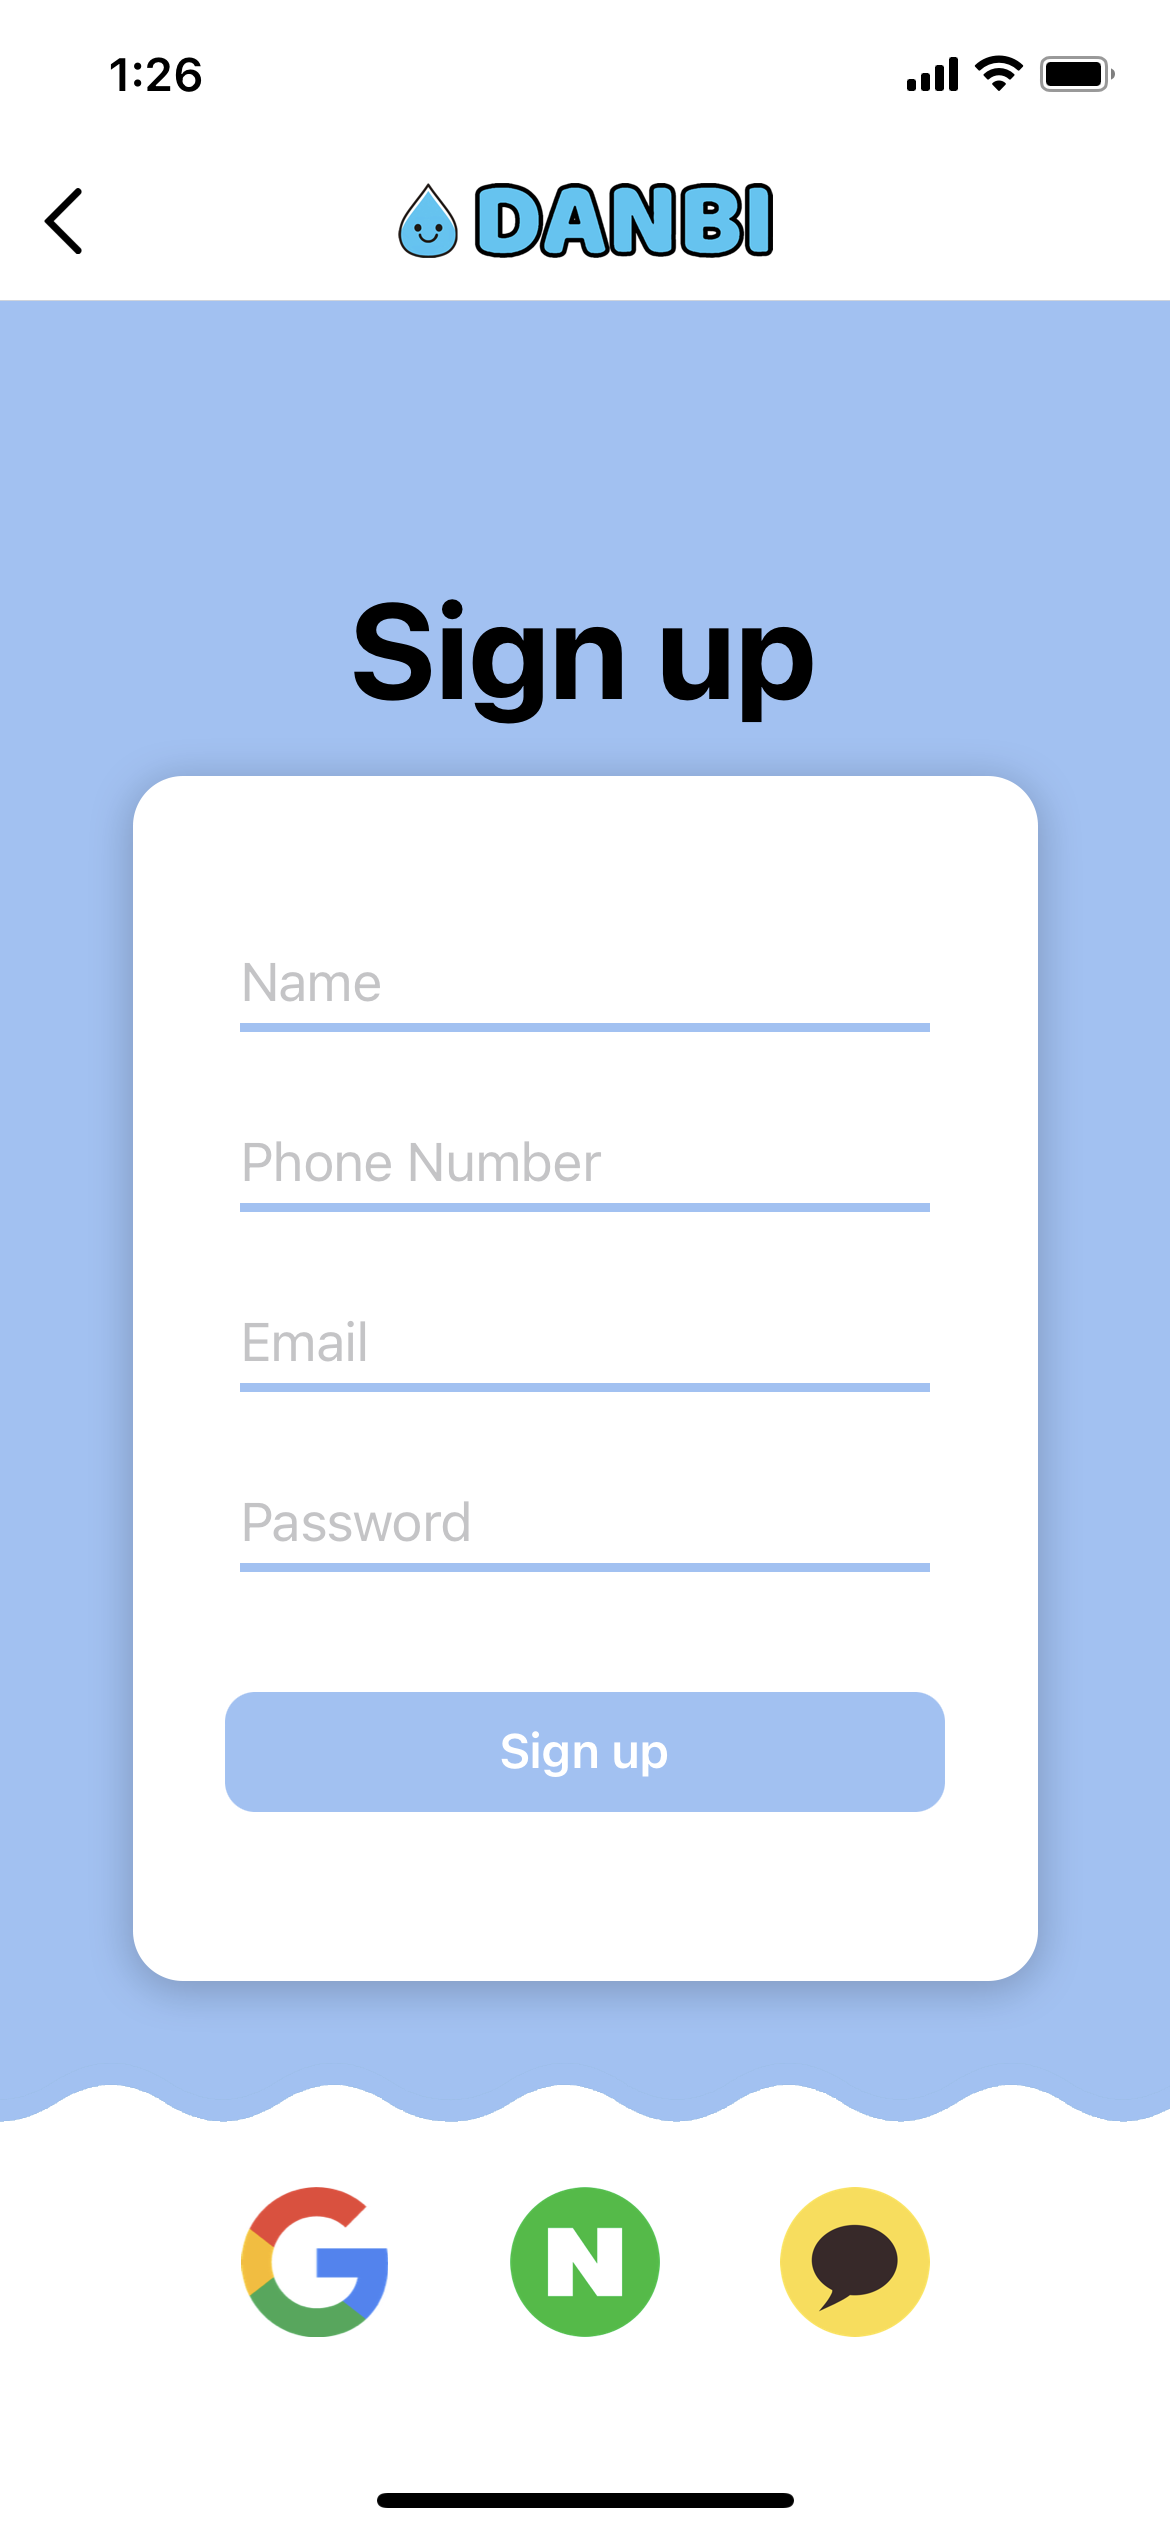
\includegraphics[width=3cm]{page/signUp.png}
\centering
\caption{Sign up}
\label{fig:signup}
\end{figure}

[Fig. \ref{fig:signup}] At the bottom of the 'Login page', user can access the 'Sign Up page' through the sign-up button and can register to DANBI. DANBI provides a general membership function and a membership function through social accounts. The user's information required in the membership registration includes a name, mobile phone number, Email address, and Password.
\begin{enumerate}
\setlength{\parindent}{2ex}
\item Social Sign Up

Social accounts available include 'Google', 'NAVER', and 'Kakao'. When using the social login function, the account is registered with the social ID and Password without a separate authentication procedure. The user's name, mobile phone number, and Email information must be received from a social account, and the user's consent is necessary. When the user presses the agree button, personal information is stored in the DANBI database and the account is created. If the account is successfully created, the user automatically moves back to the 'Login page'.
\item General Sign Up

User can sign up in person by entering 'name', 'mobile phone number', 'Email address', and 'Password'.
\begin{itemize}
\item Name : The name must be text. If the user presses the sign up button without entering or entering a non-text value in the name field, the error message "올바른 이름을 입력하세요." appears as pop-up in the field.

\item Mobile phone number : Mobile phone number must be a number. If the user presses the sign up button without entering or entering a non-numerical value in the mobile phone number field, the error message "올바른 핸드폰 번호를 입력하세요." appears as pop-up in the field. If the user enters the mobile phone number that has already been used for account, the error message "이미 등록된 핸드폰 번호입니다." appears pop up on the field.

\item Email address : Email address must be in the form of an Email. If the user presses the sign up button without entering or entering a value that is not in the form of an Email in the field, the error message "올바른 이메일 주소를 입력하세요." appears as pop up in the field. If the user enters the email address that has already been used for account, the error message "이미 등록된 이메일 주소입니다." appears pop up on the field.
\item Password : Password must satisfy 6-10 digits by combining letters and numbers. If you press the sign up button without entering or entering a Password that doesn't satisfy the conditions in the password field, the error message "올바른 비밀번호를 입력하세요." appears as pop-up in the field. The same process is repeated in the Password verification field. If different values are entered in the Password field and Password verification field, the error message appears pop up in the Password verification field.
\end{itemize}
After entering all input values without errors and pressing the sign up button, 'name', 'ID', 'mobile phone number', 'Email address', 'Password' information is stored in the DANBI database and a new account is created. The application automatically provide the 'Login page'.
\end{enumerate}

\item \textbf{Login Page / Forgot ID / Forgot Password}

\par \begin{figure}[h!]
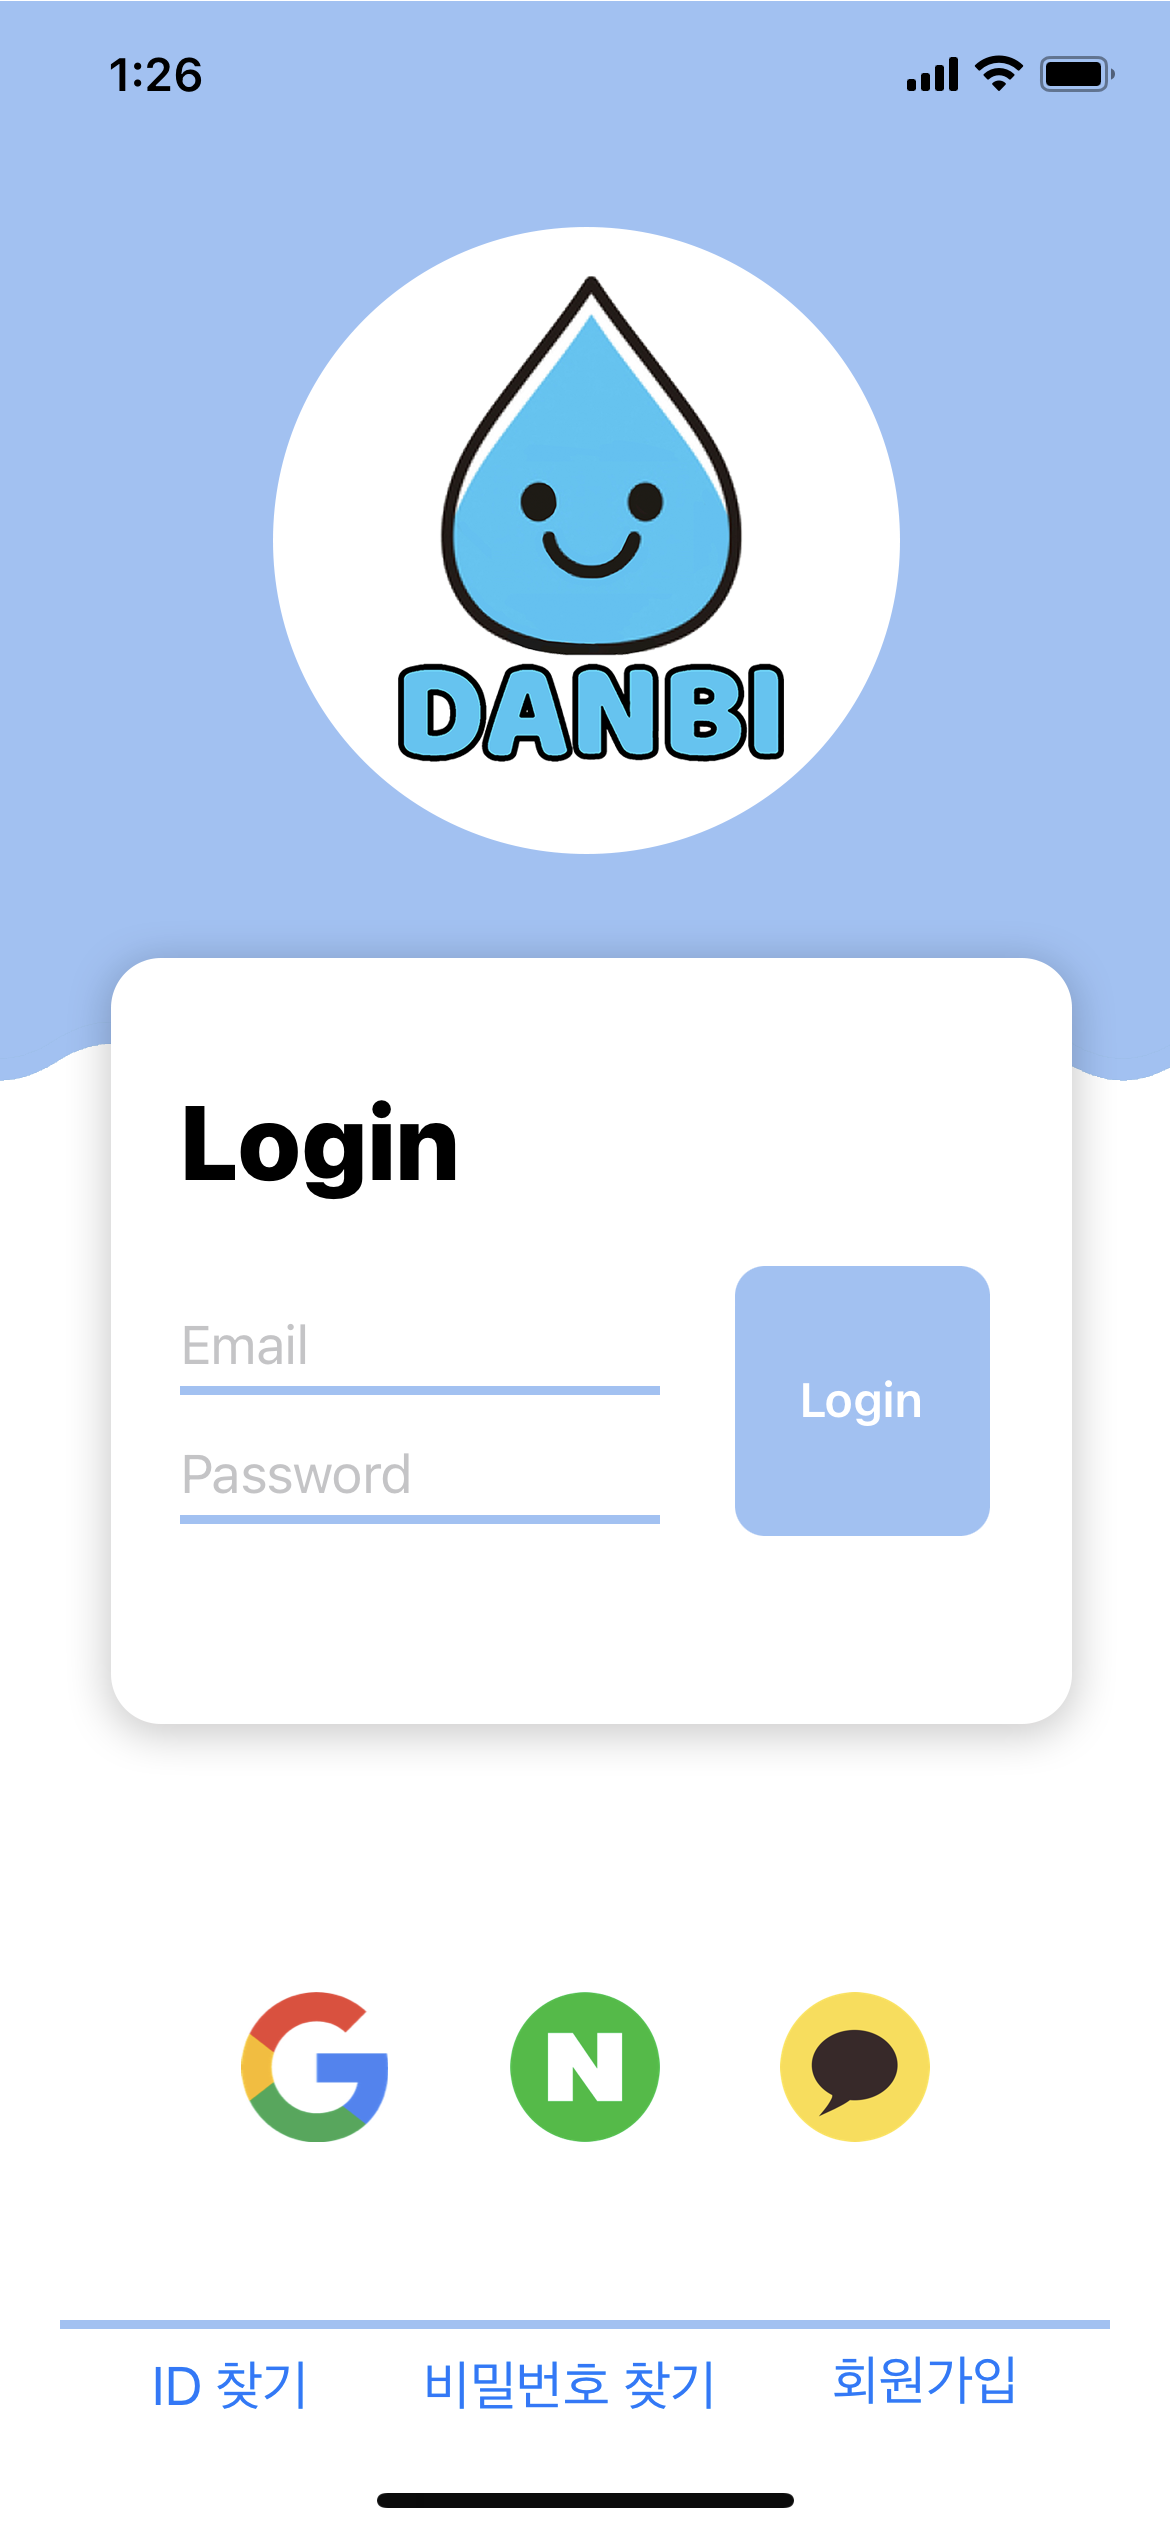
\includegraphics[width=3cm]{page/login.png}
\centering
\caption{Login}
\label{fig:login}
\end{figure}

\par \begin{figure}[h!]
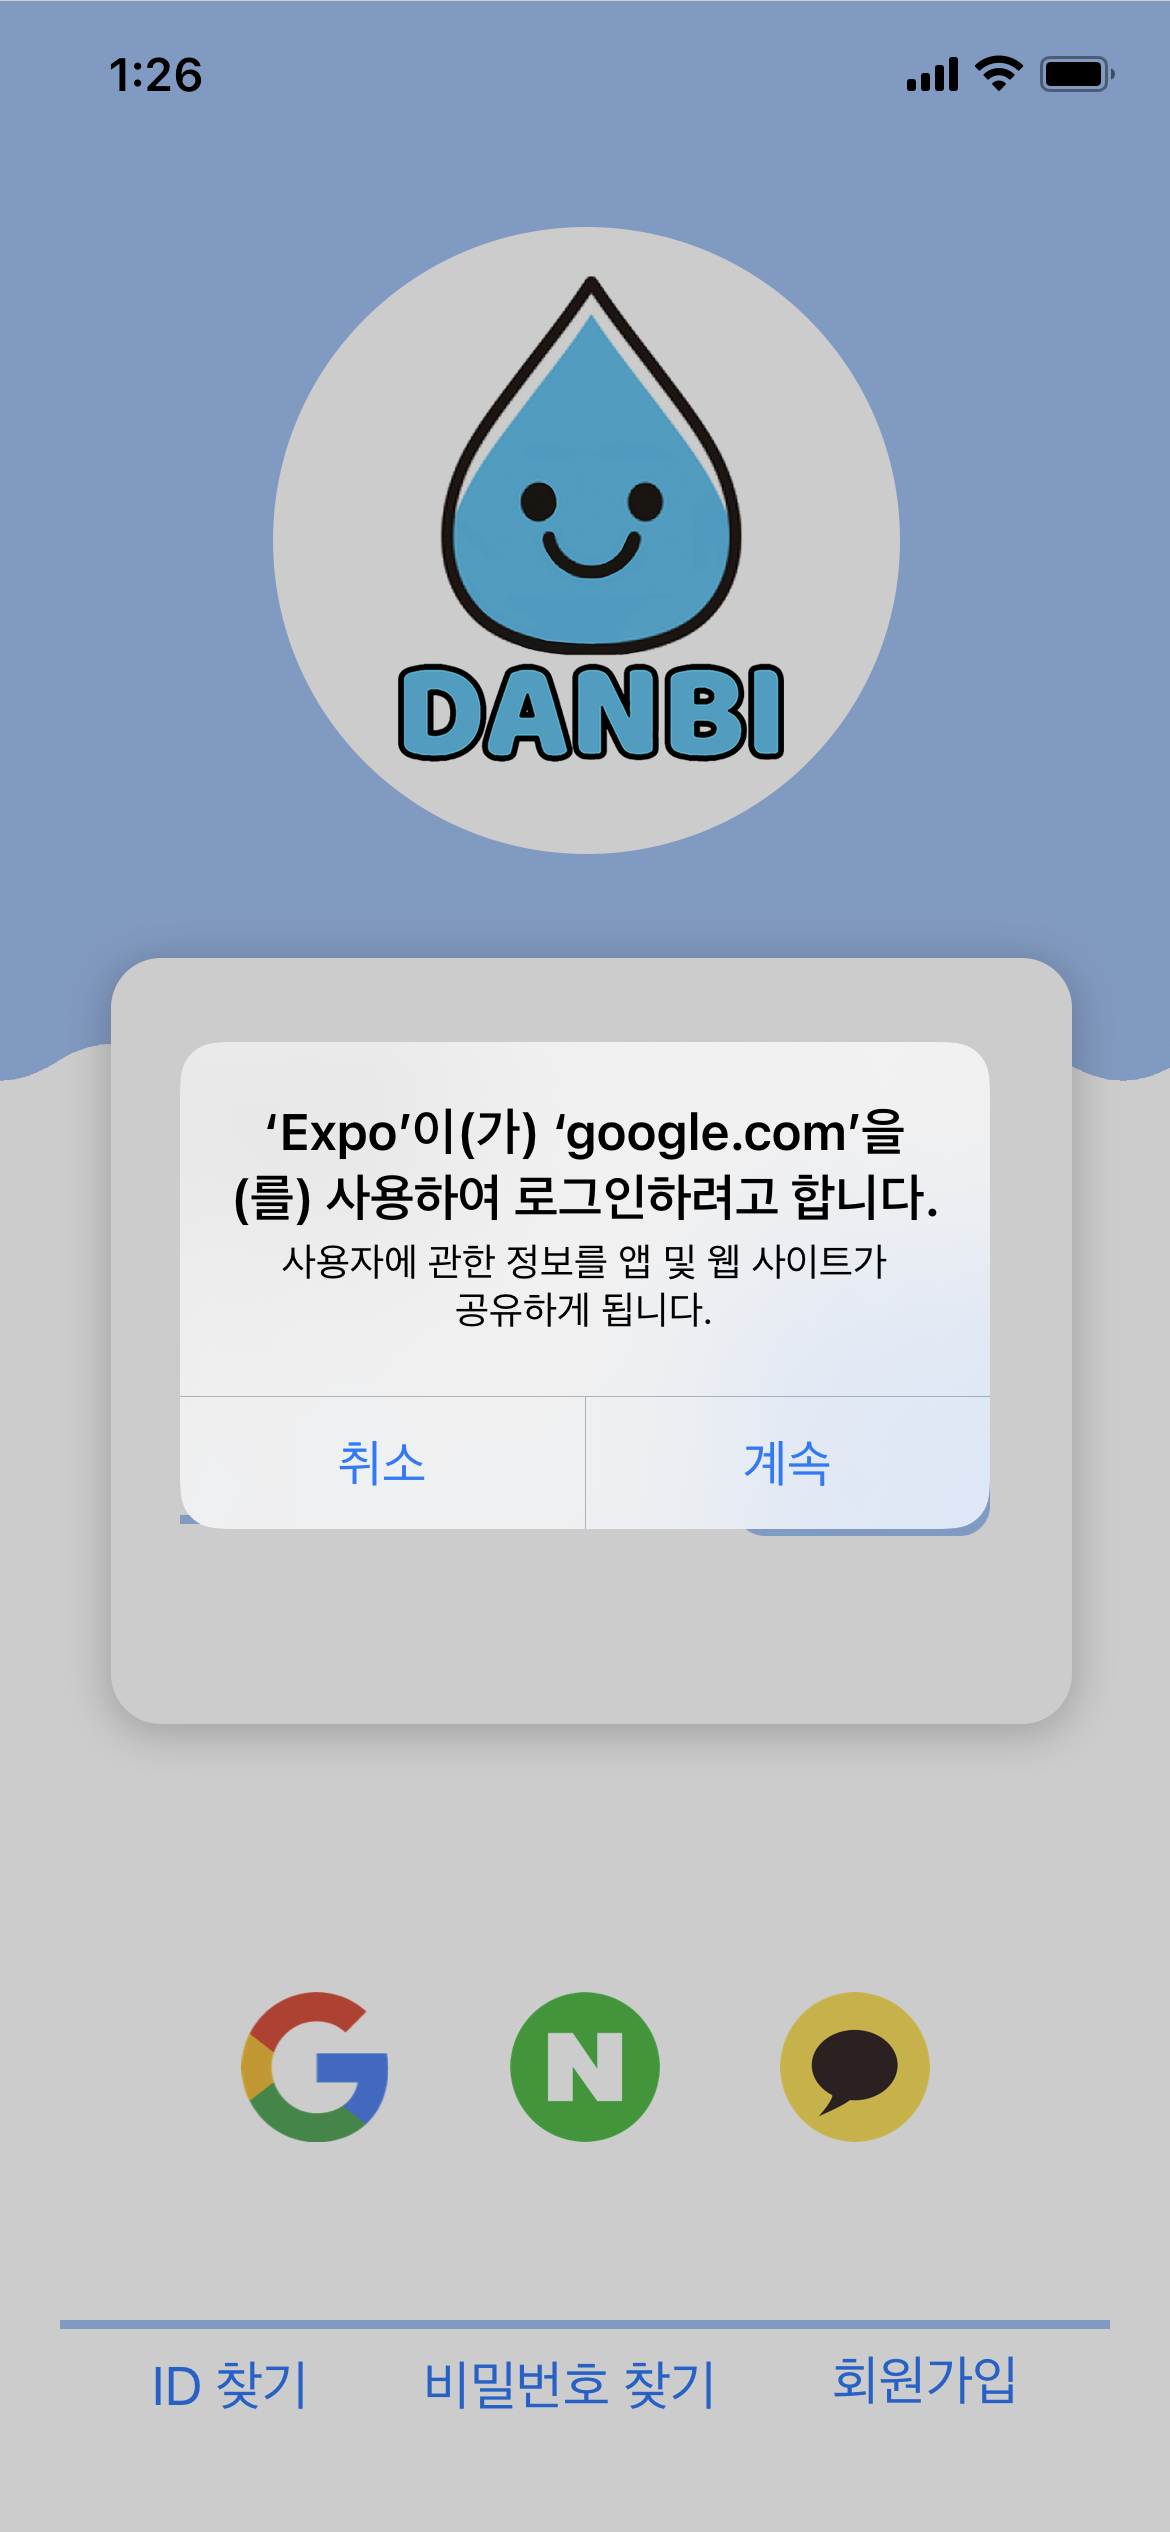
\includegraphics[width=3cm]{page/GoogleLogin.png}
\centering
\caption{Google Login}
\label{fig:GoogleLogin}
\end{figure}

\par \begin{figure}[h!]
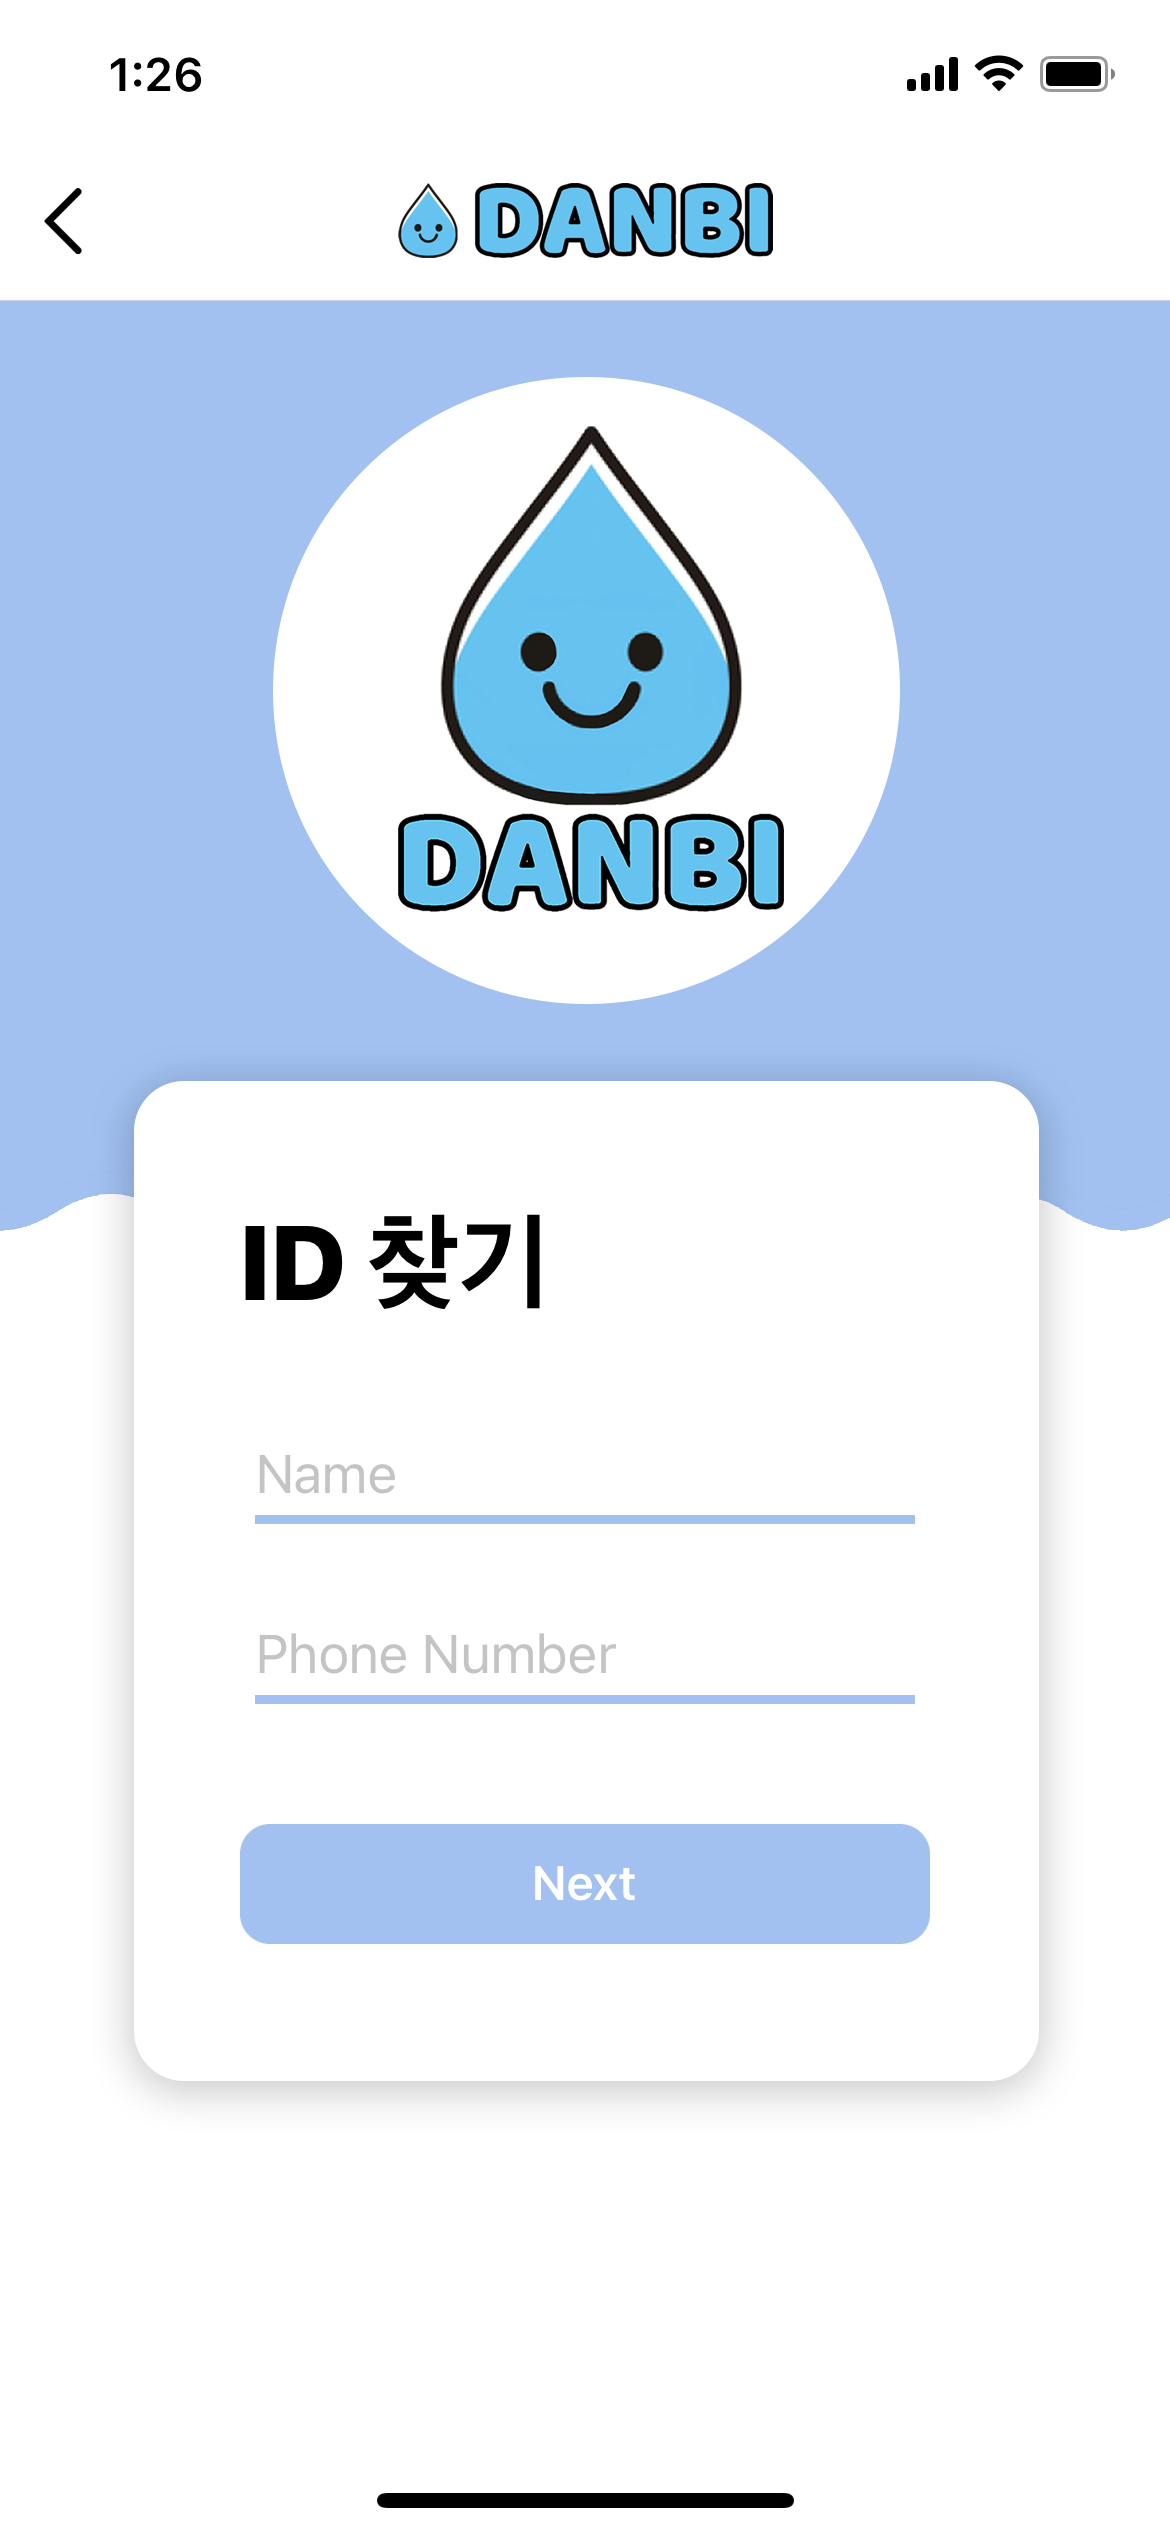
\includegraphics[width=3cm]{page/forgotID.png}
\centering
\caption{Forgot ID}
\label{fig:forgotID}
\end{figure}

\par \begin{figure}[h!]
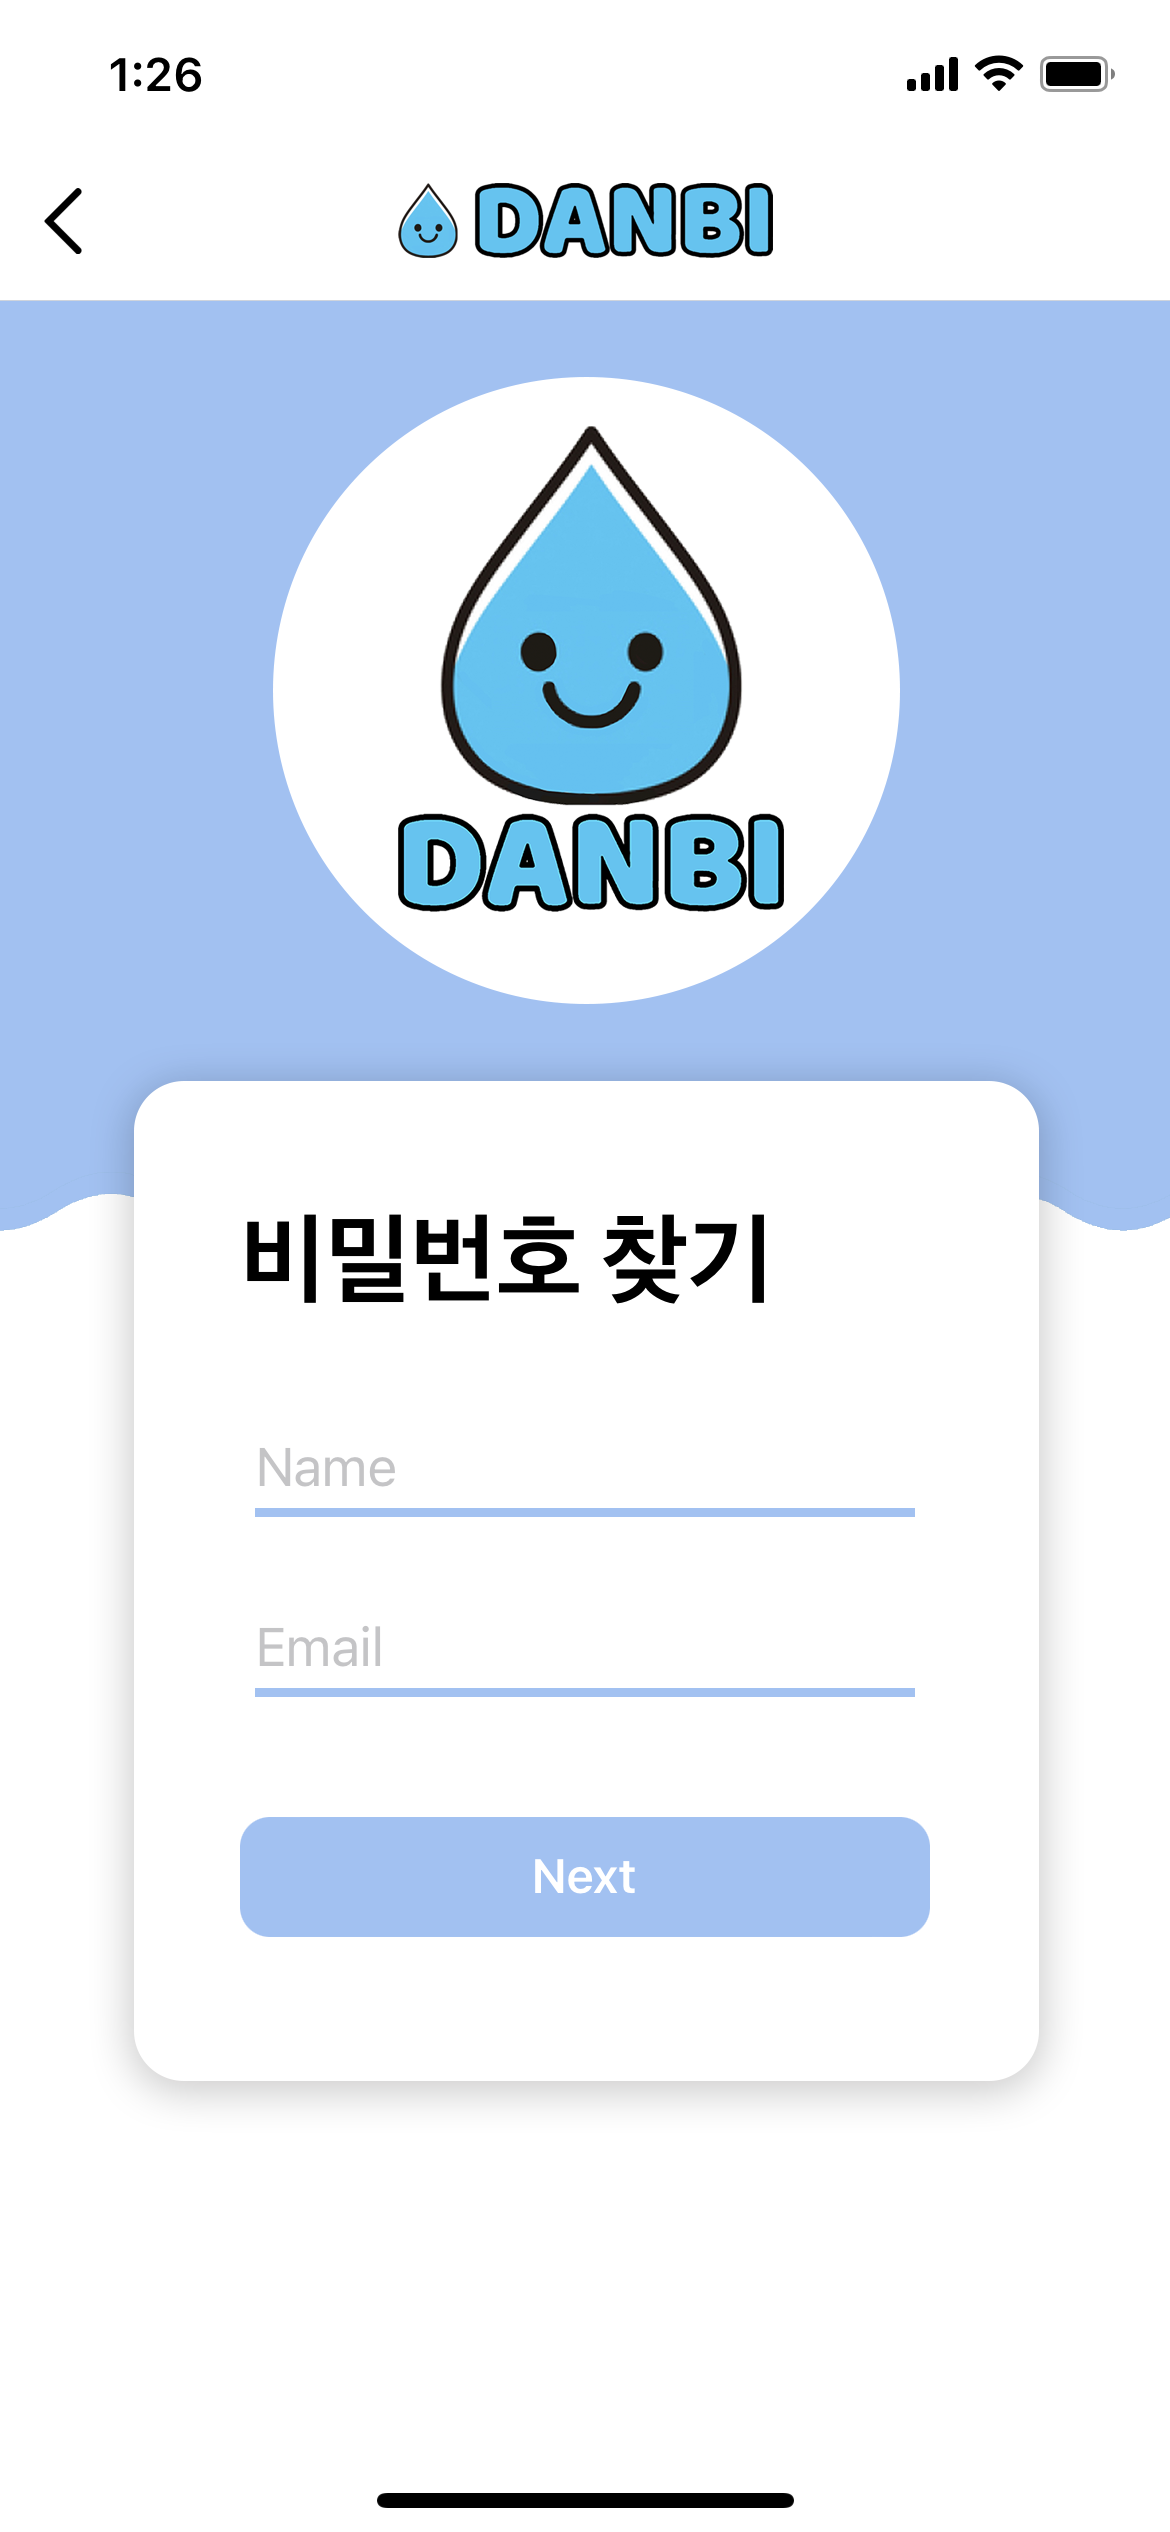
\includegraphics[width=3cm]{page/forgotPW.png}
\centering
\caption{Forgot PW}
\label{fig:forgotPW}
\end{figure}

\par \begin{figure}[h!]
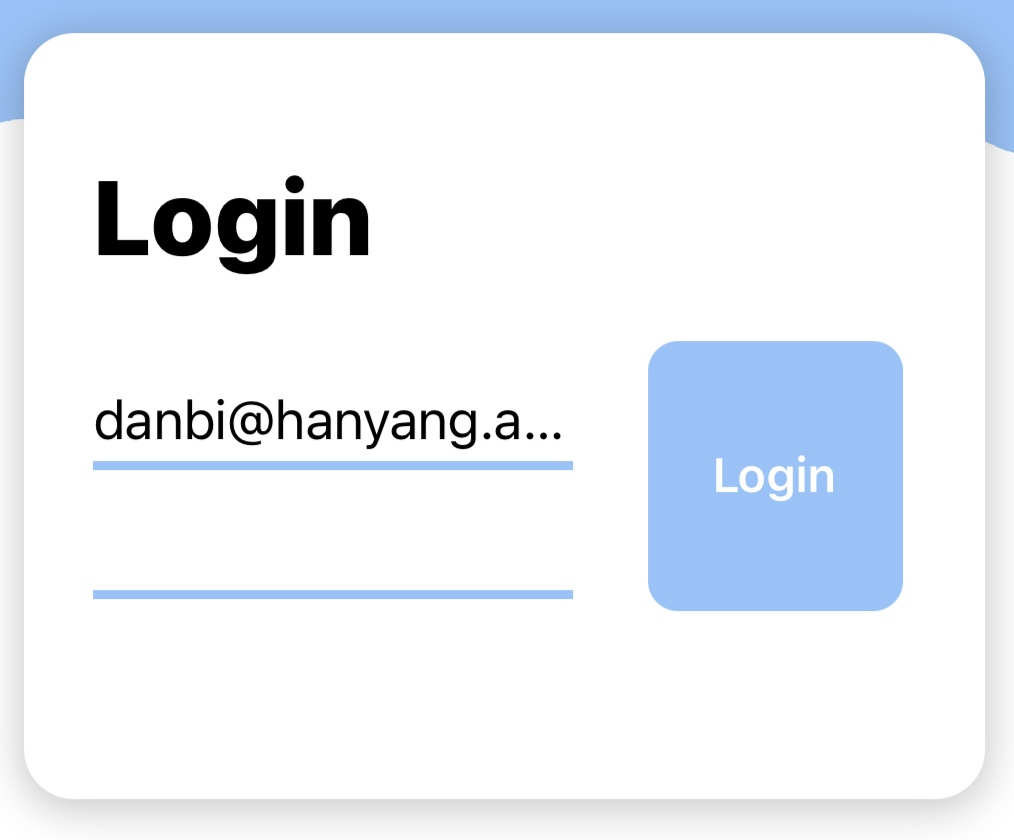
\includegraphics[width=3cm]{image/PW.jpg}
\centering
\caption{Protection of PW}
\label{fig:Protection of PW}
\end{figure}

[Fig. \ref{fig:login}] There are two text fields(Email, Password) in the 'Login page'. The user may log in by entering an Email and Password in the corresponding field. In the case of the Password field, the input value is changed as a dot(When capture the screenshot, there is a function that can't see dot shape [Fig. \ref{fig:Protection of PW}]). There is a login button on the right side of the text field. Under the two fields and login button, there are icons of 'Google' [Fig. \ref{fig:GoogleLogin}], 'NAVER' and 'Kakao' that allow social login. If you press the login button after entering the correct information, application automatically provide the 'Main page'. At the bottom, there are find ID, find Password, and sign up buttons. If the user presses the sign up button, application automatically access the 'Sign Up page'. Account information can be recovered by touching finding ID [Fig. \ref{fig:forgotID}] and finding Password [Fig. \ref{fig:forgotPW}] at the bottom.

\begin{enumerate}
\setlength{\parindent}{2ex}
\item Correct ID and Password

Account information is sent to the database when the user correctly enters the ID value(Email), Password and presses the login button. Database sends the data values stored about account to the server and processes them so that the application can show the data to the user. During this process, an ActivityIndicator(loading icon) is displayed. If the user log in successfully, the ActivityIndicator automatically disappears and the user accesses the 'Main page'.

\item Wrong ID or password

If the account information entered in the text field is not in the database, the error message "계정 정보가 없습니다. 아이디나 비밀번호를 확인해주세요." appears as pop up in the field. If the user touches to modify the field, the existing input value is automatically erased.

\item Account retrieval

Account information can be recovered by touching finding ID or finding Password at the bottom. If the user forgets the Email address registered with ID, she can recover it by entering the name and mobile phone number. The entered information is sent to the server, and database returns the account Email address that matches to information. The password is not a method of bringing up values stored in the database, but a method of registering a new Password. If the user forgets the Password, entering the ID and name will send the authentication code to the entered Email. Authenticating the code allows the user to set a new password. If the application have processed all the ID or Password changes requested by the user, it will automatically access the 'Login page' again.

\end{enumerate}

\item \textbf{Main Page}

\par \begin{figure}[h!]
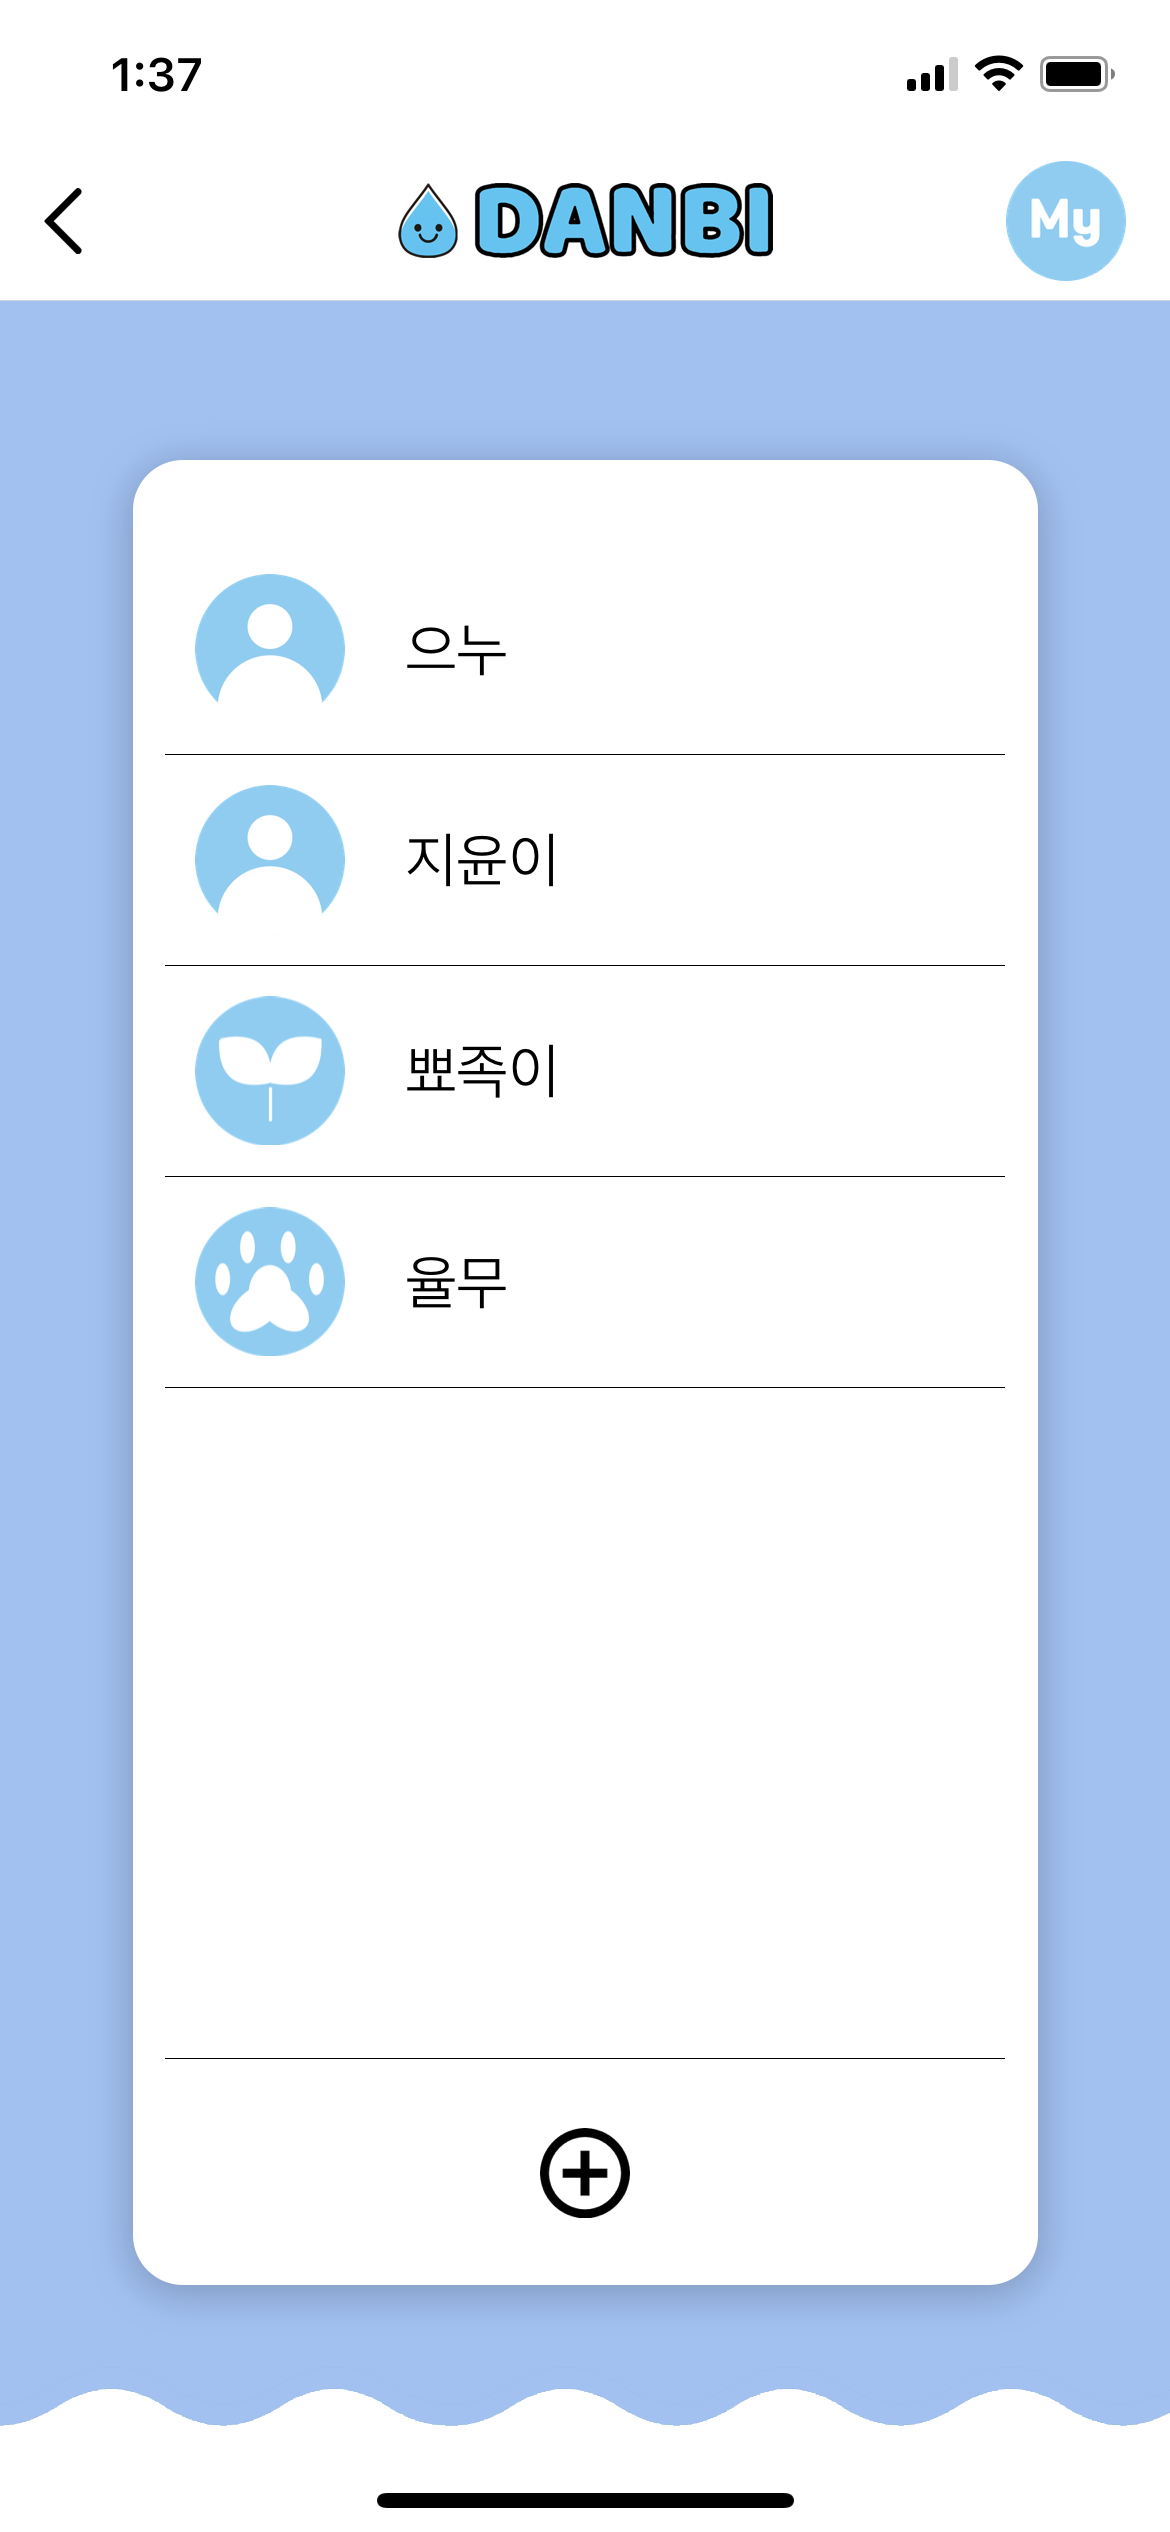
\includegraphics[width=3cm]{page/main.png}
\centering
\caption{Main page}
\label{fig:main}
\end{figure}

[Fig. \ref{fig:main}] In 'Main page', the user can see a list of members registered in account. In DANBI, humans, pets, and plants can be registered as family members. The member's nickname is provided in the form of a list along with an icon representing each object, and when each nickname is clicked, the member's detailed screen page is accessed. There is a '+' button below the member list. When the button is clicked, application is automatically connected to the 'Member Registration page' where user can add members.

\item \textbf{My tab}

\par \begin{figure}[h!]
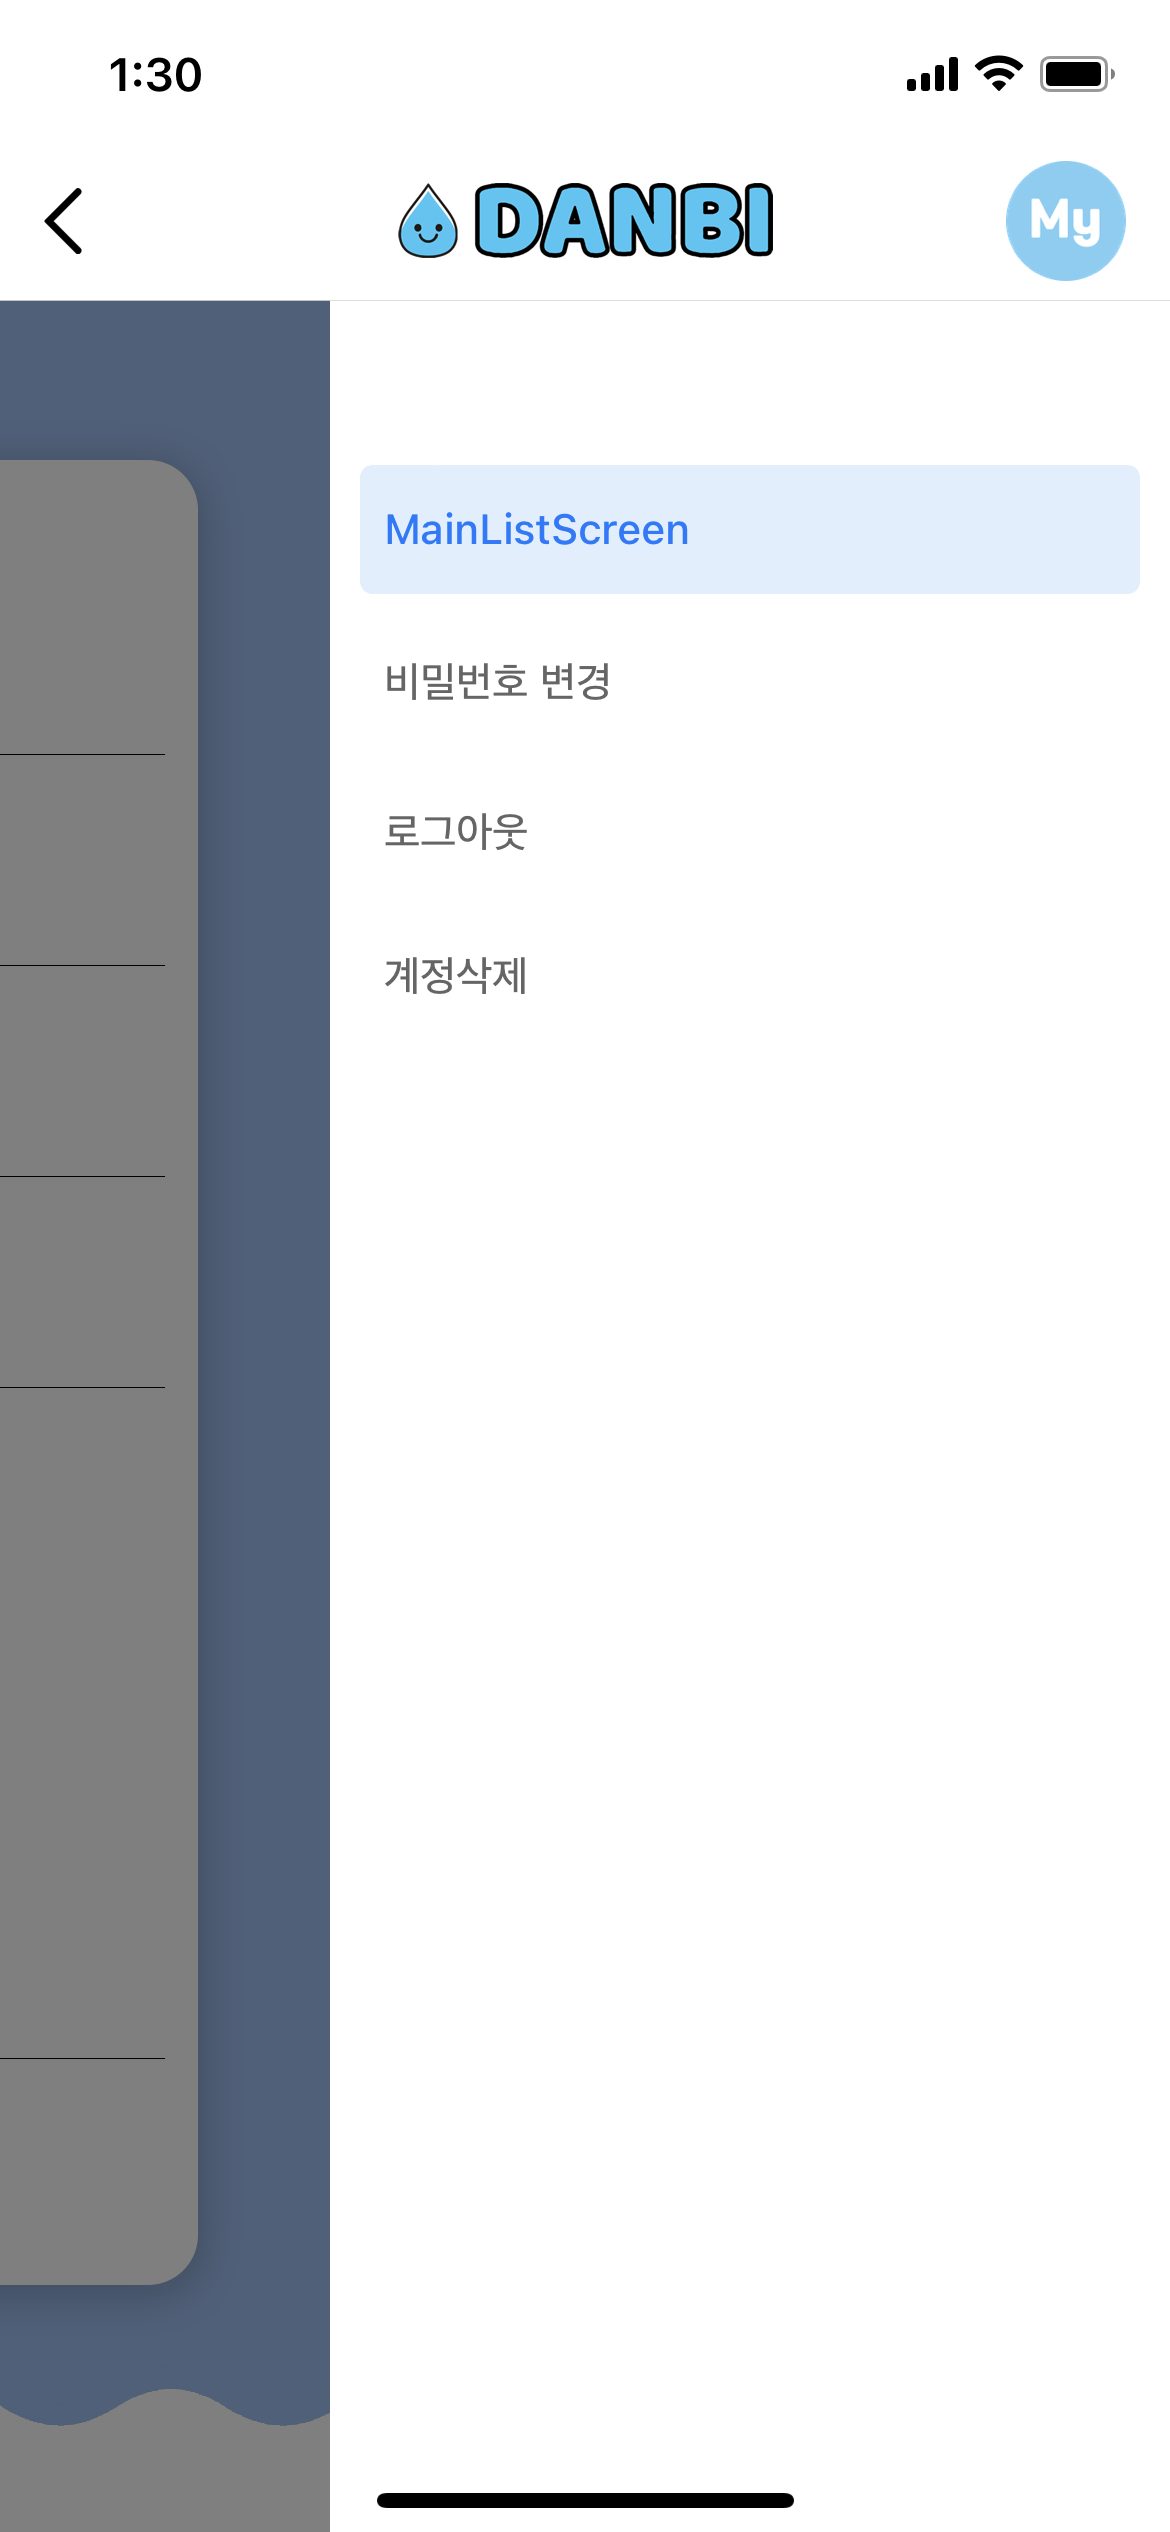
\includegraphics[width=3cm]{page/MYtab.png}
\centering
\caption{Mytab drawer}
\label{fig:mytab}
\end{figure}

\par \begin{figure}[h!]
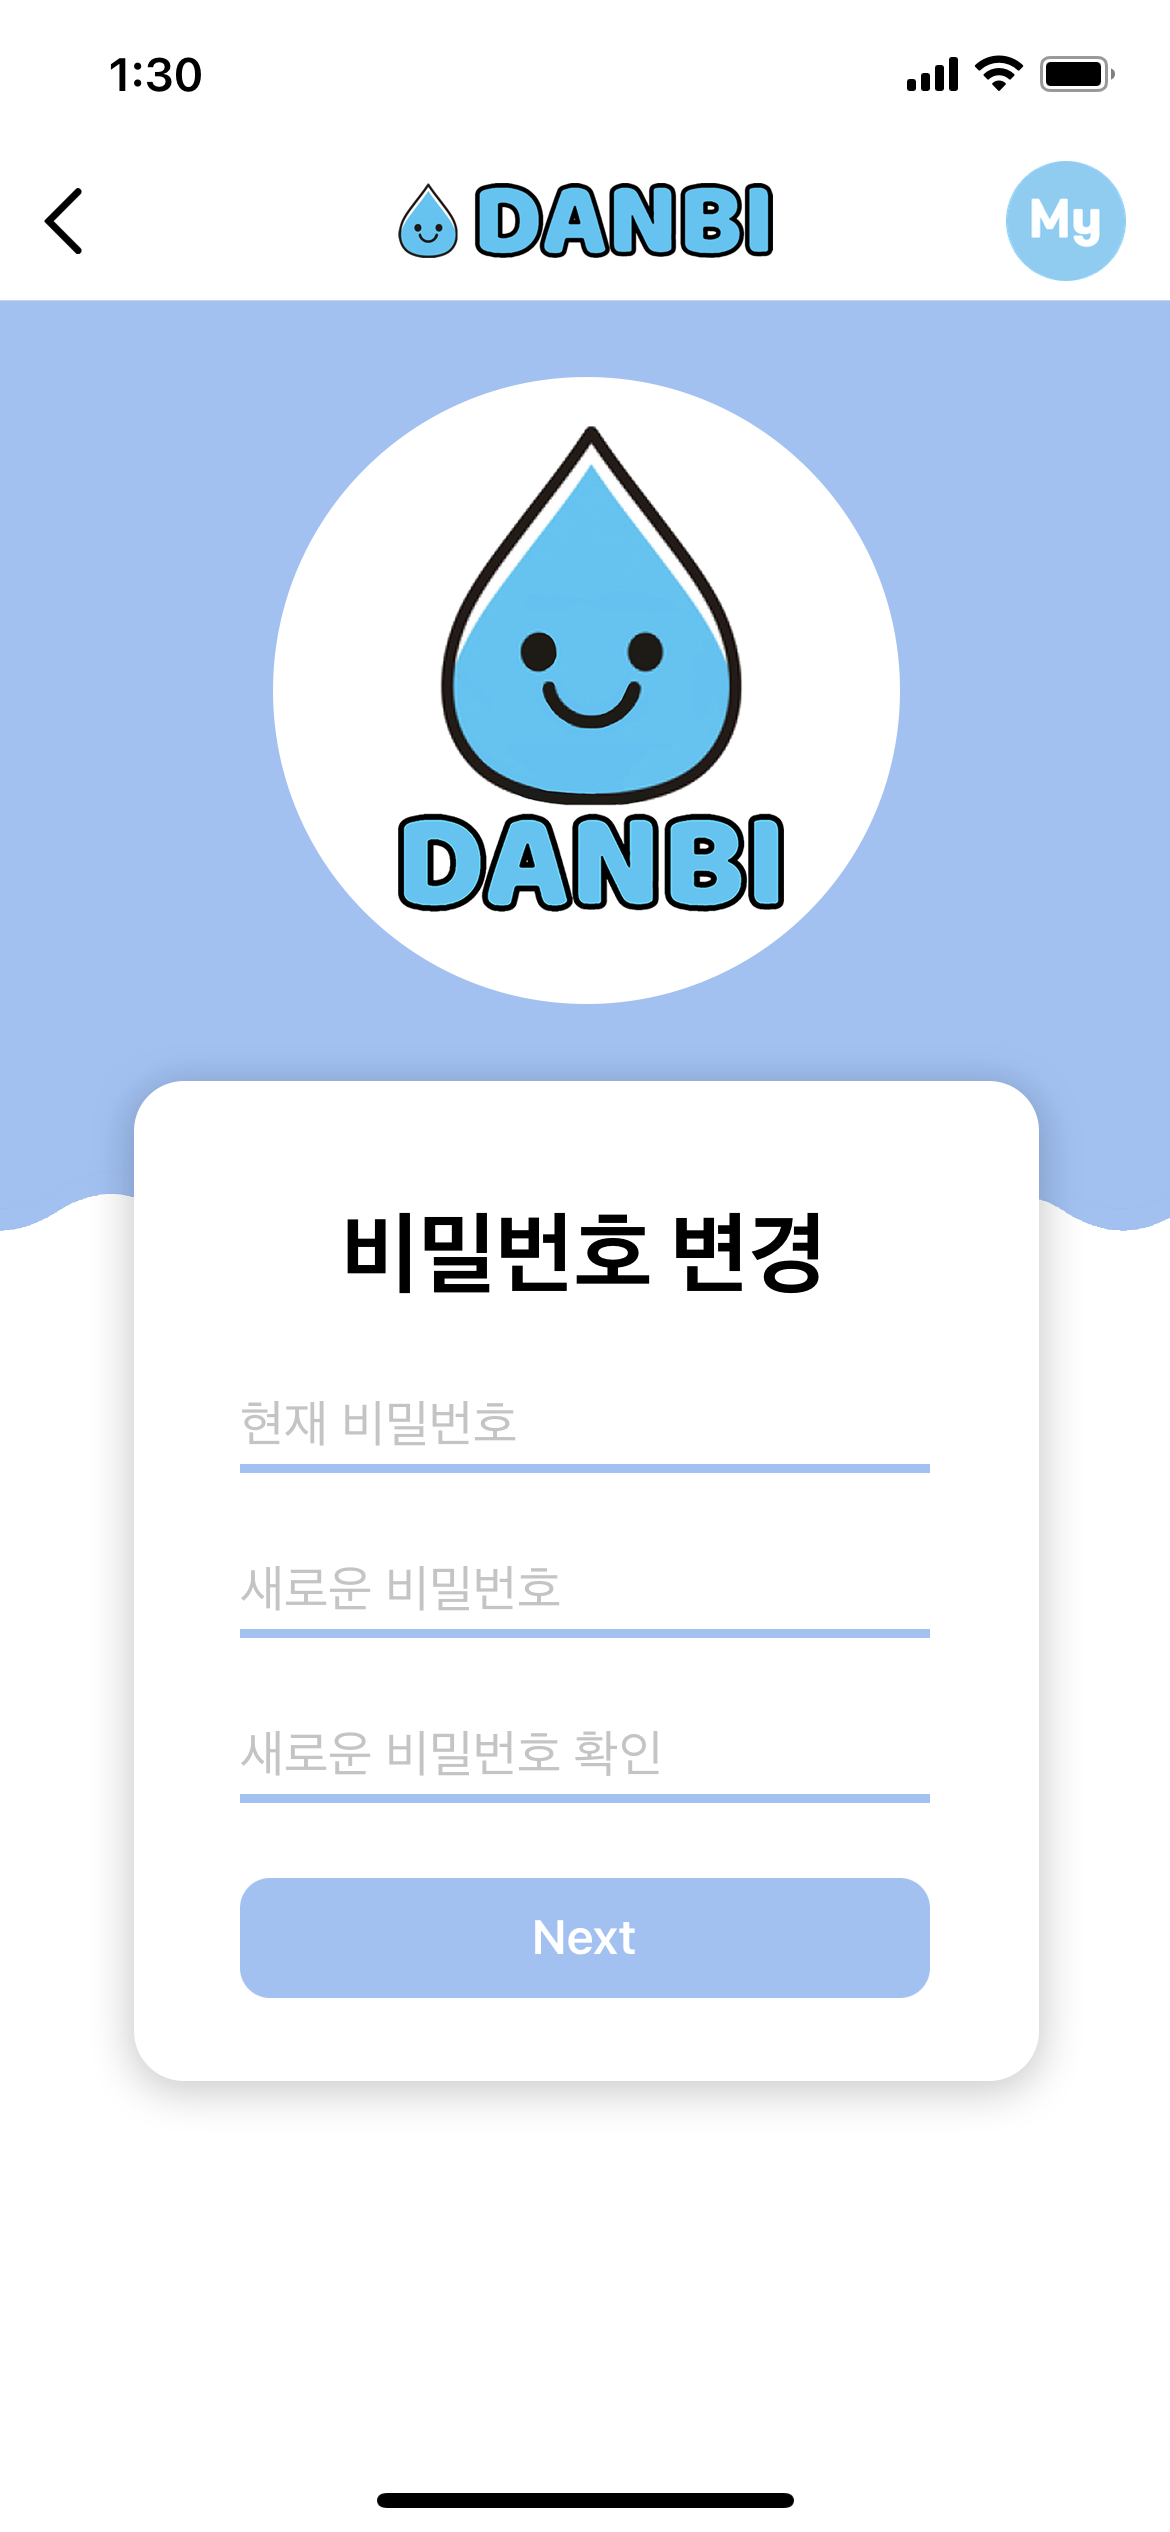
\includegraphics[width=3cm]{page/changePW.png}
\centering
\caption{Change PW}
\label{fig:changePW}
\end{figure}

\par \begin{figure}[h!]
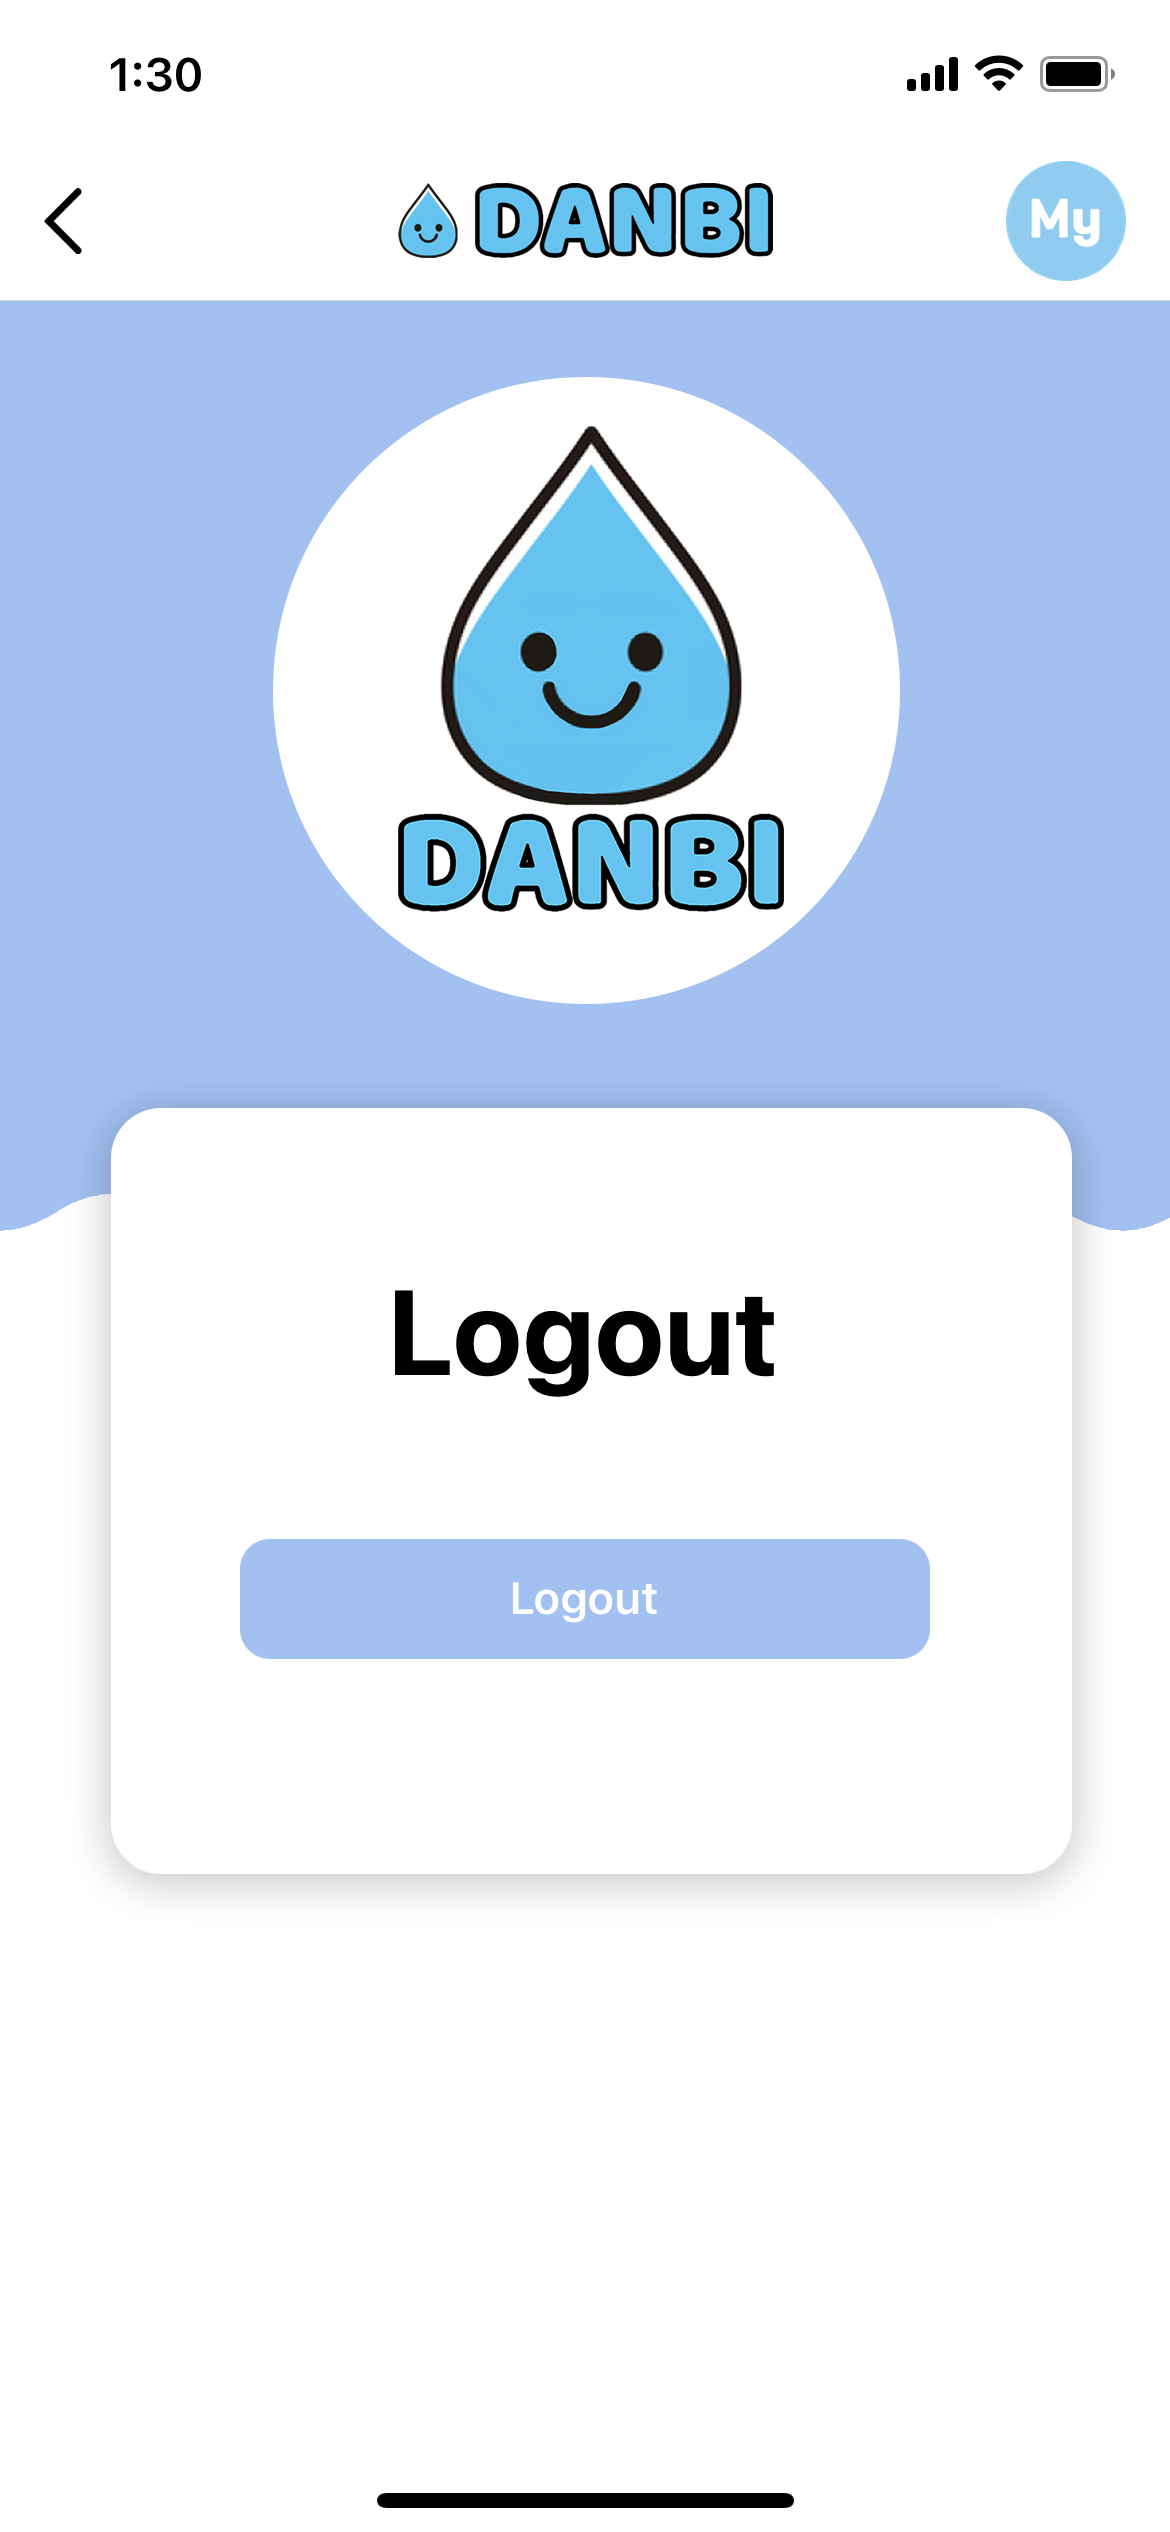
\includegraphics[width=3cm]{page/logout.png}
\centering
\caption{Logout}
\label{fig:logout}
\end{figure}

\par \begin{figure}[h!]
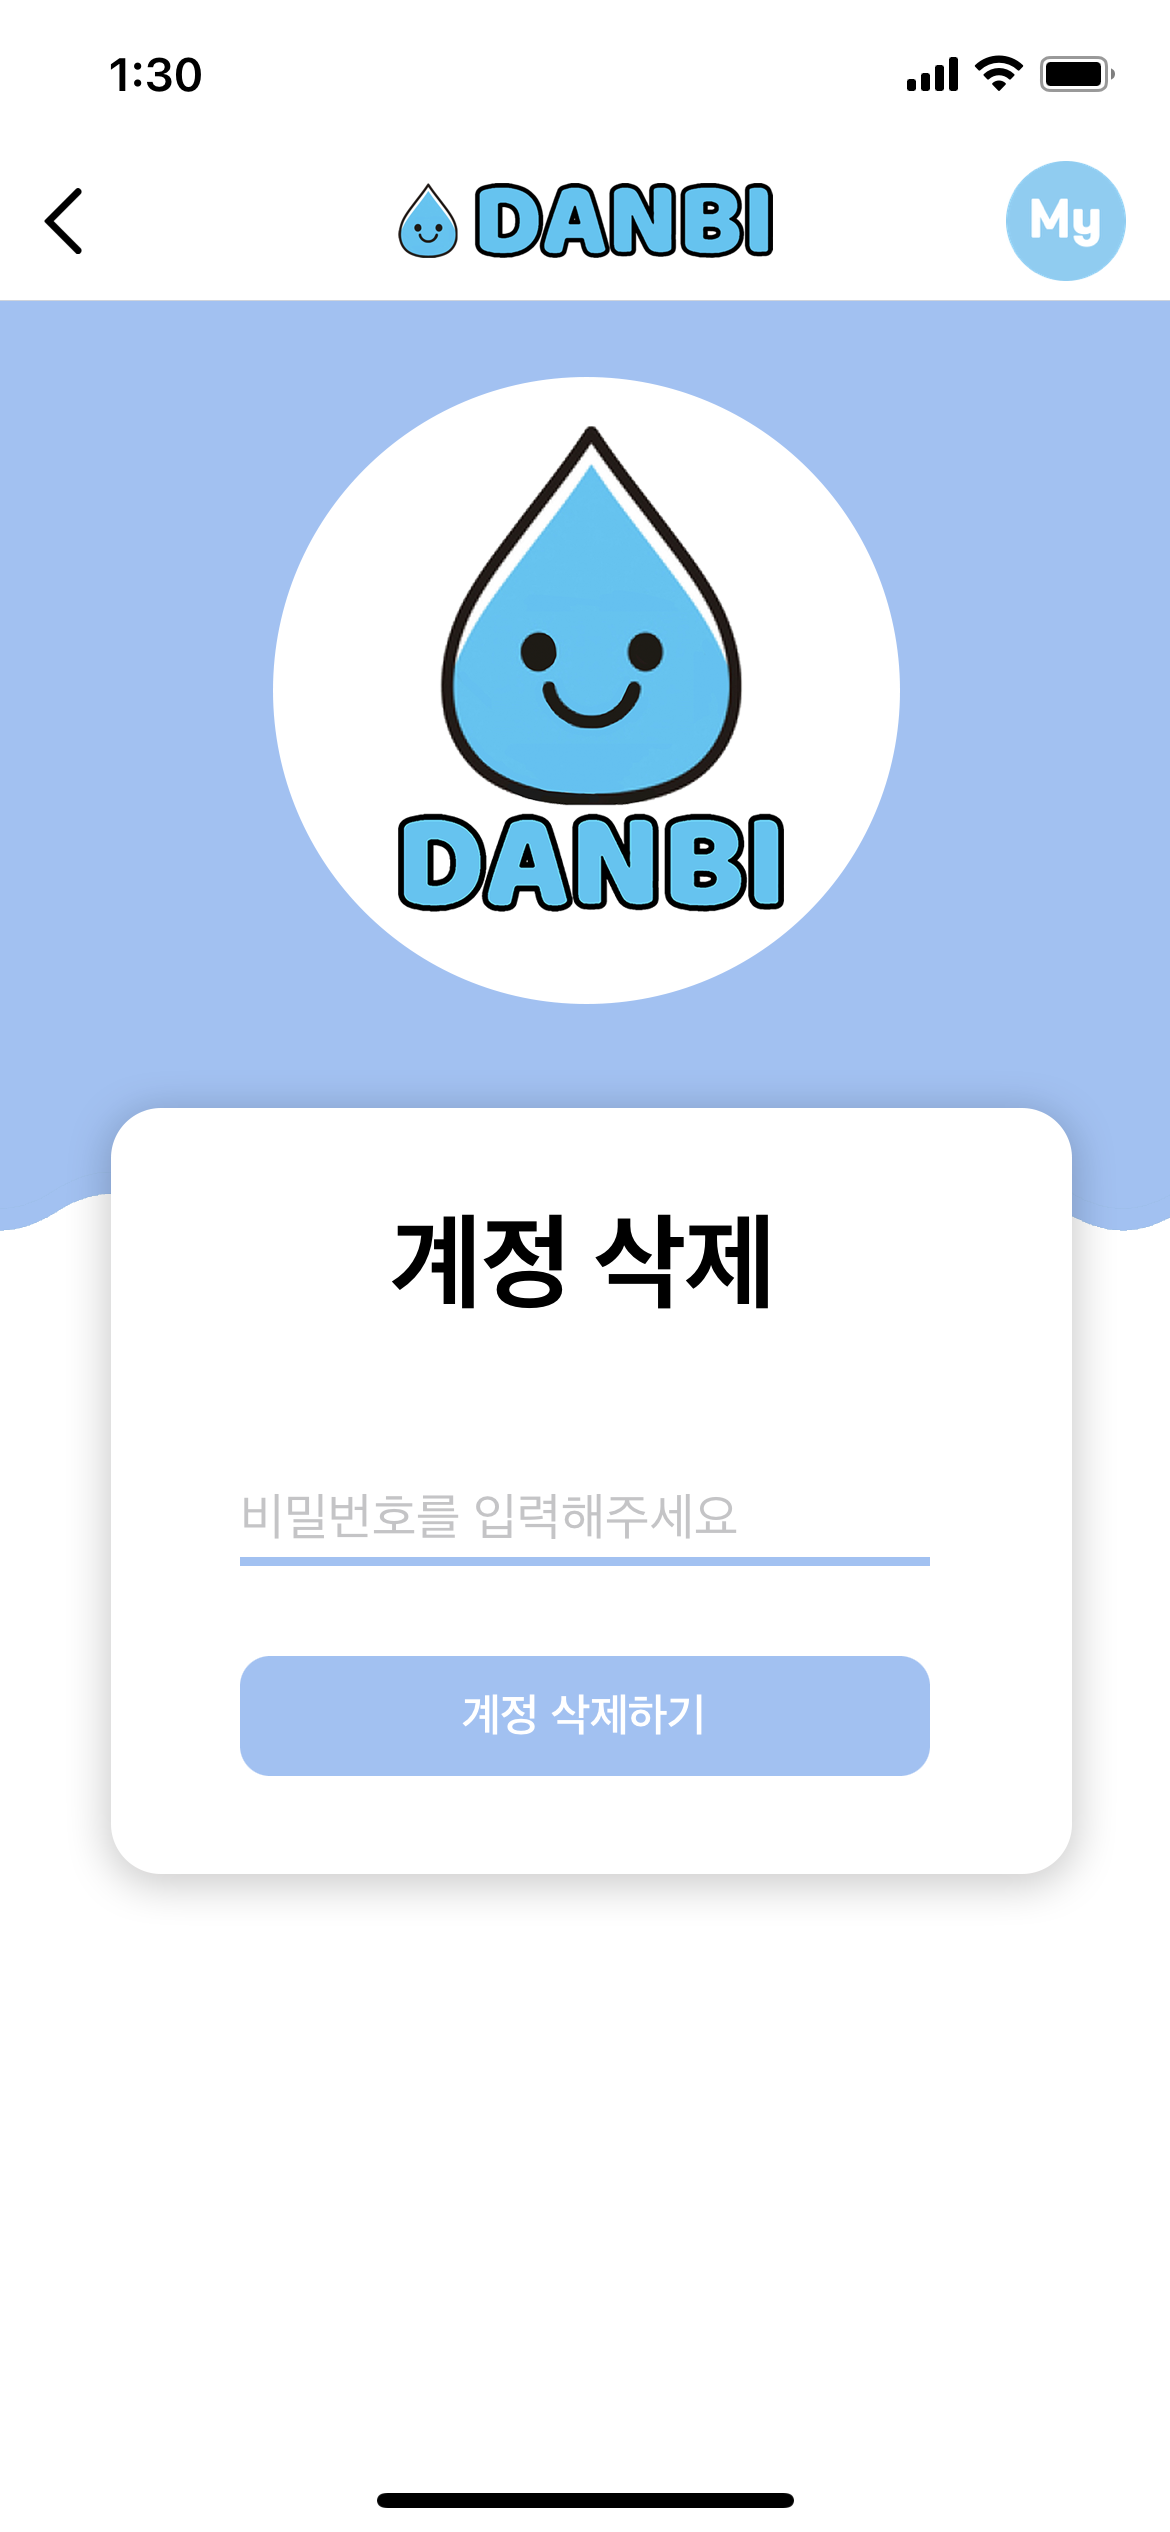
\includegraphics[width=3cm]{page/deleteAccount.png}
\centering
\caption{Delete account}
\label{fig:deleteAccount}
\end{figure}

[Fig. \ref{fig:mytab}] 'My tab' can be accessed through a drawer or by pressing the sky blue 'My' button at the top of the 'Main page'. In this tab, there are main page, change password [Fig. \ref{fig:changePW}], logout [Fig. \ref{fig:logout}], and delete account [Fig. \ref{fig:deleteAccount}]. If you click each component, you can enter the page what you clicked. Specifically, registered Email information may be checked and the Password may be changed through an authentication procedure. Logout is also possible, and when the user re-access to account after logging out, the user will be connected the "Login page" after the "Entry page" and have to log in to retrieve account information again. When deleting an account, all data of the user is deleted from the database.


\item \textbf{Member registration page}

In the 'Member Registration page', information on new family members can be registered. The registered information is stored in the database and immediately added to the 'Main page', member list.
\begin{enumerate}
\setlength{\parindent}{2ex}
\item Human

\par \begin{figure}[h!]
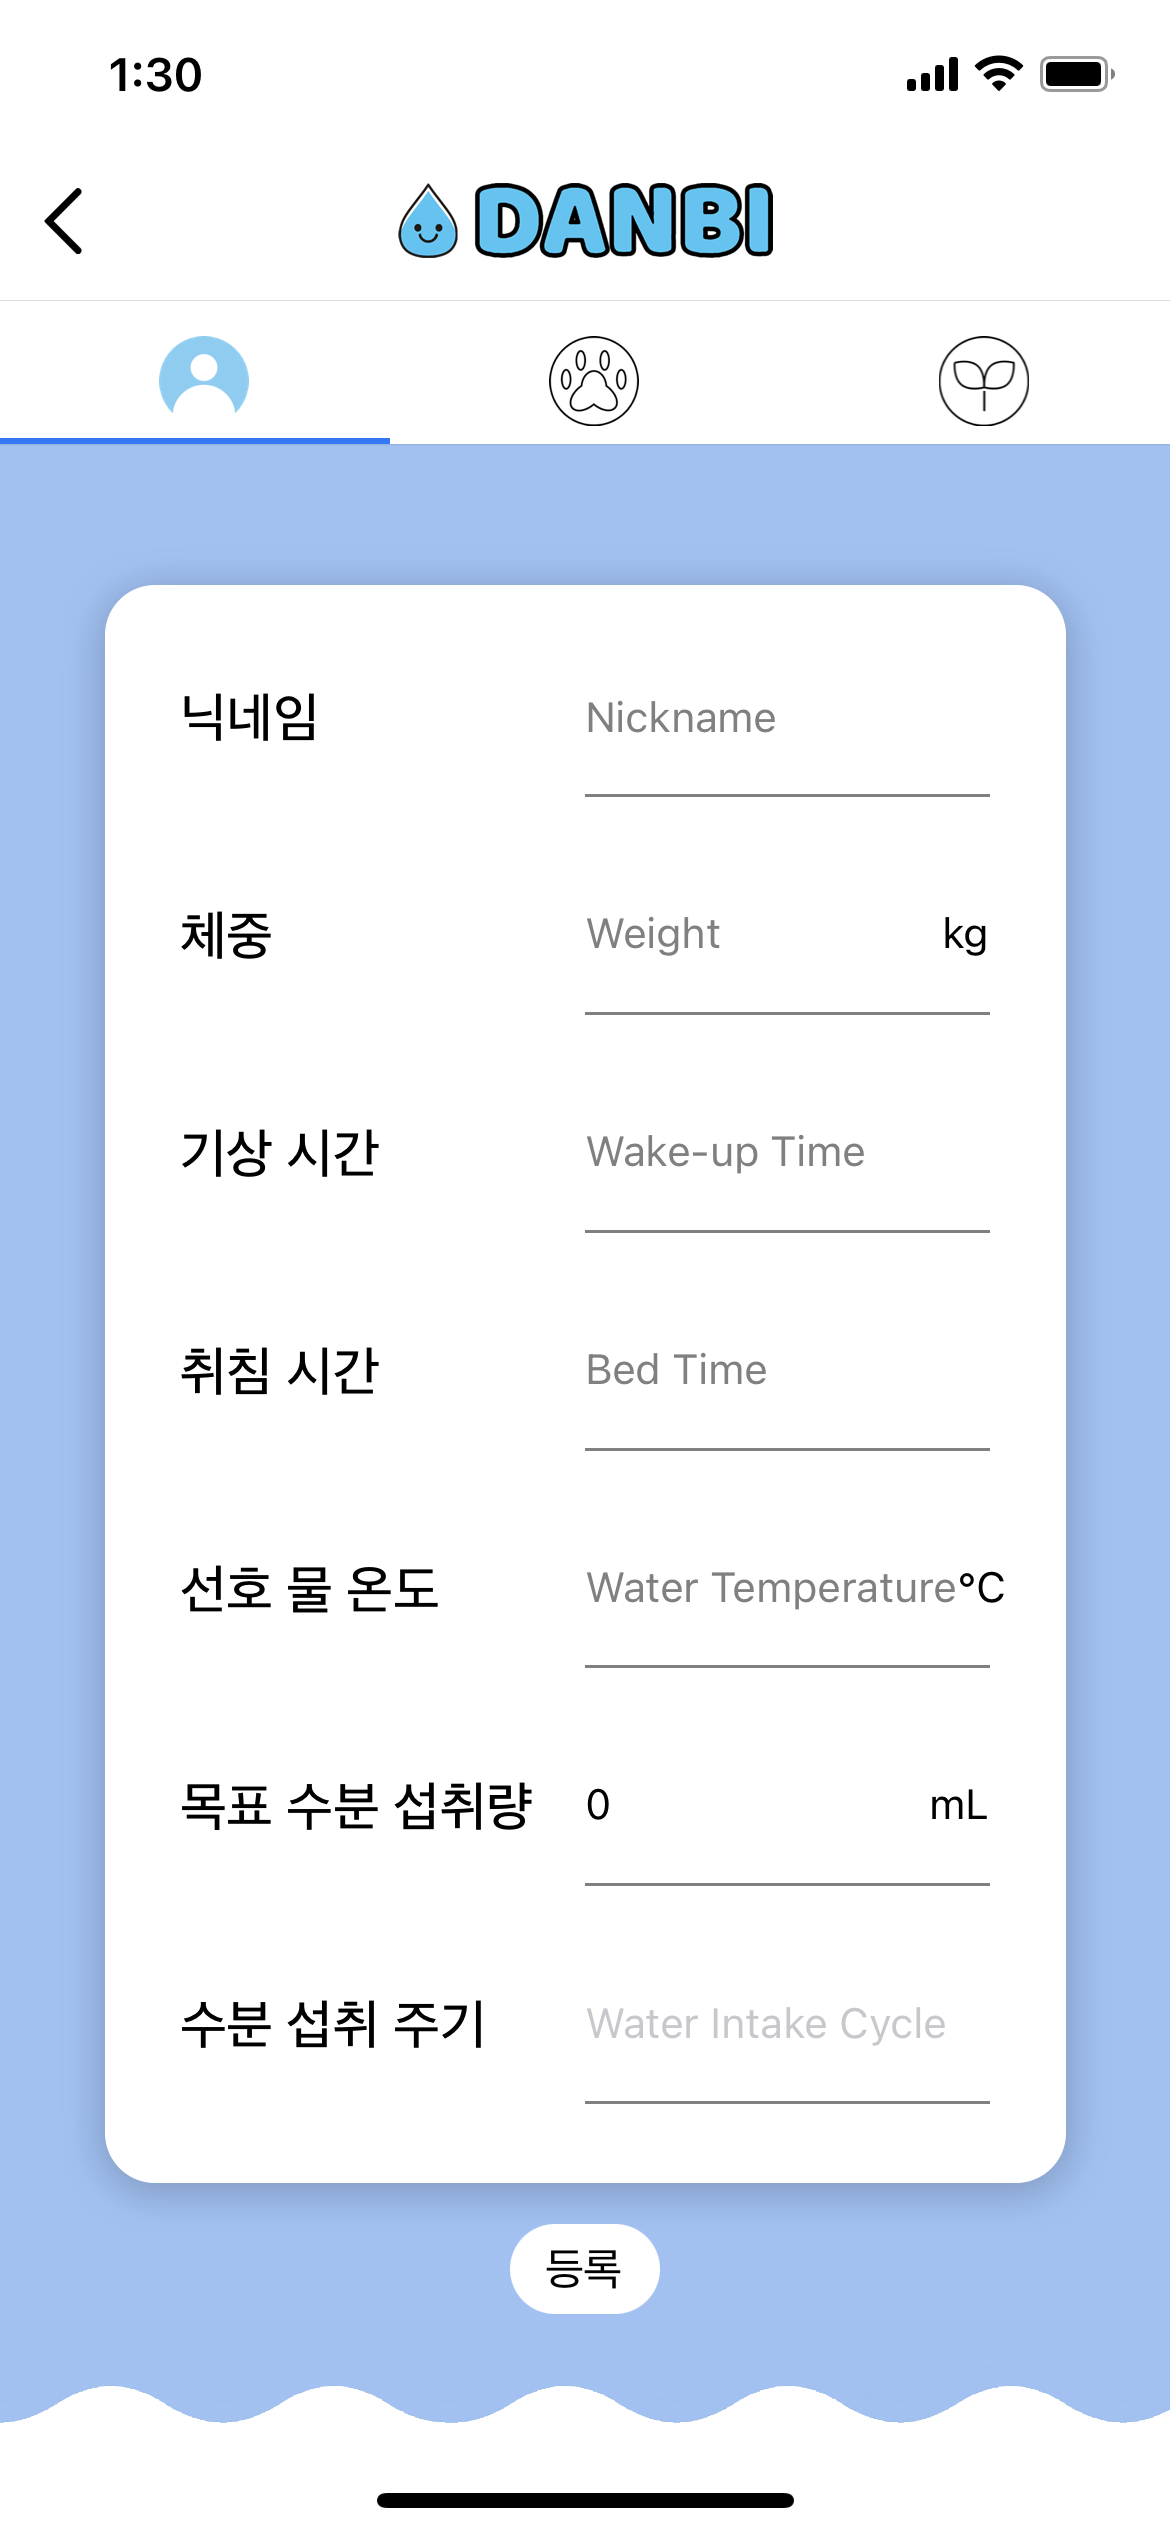
\includegraphics[width=3cm]{page/regiPerson.png}
\centering
\caption{Registration\_Person}
\label{fig:regiPerson}
\end{figure}

\par \begin{figure}[h!]
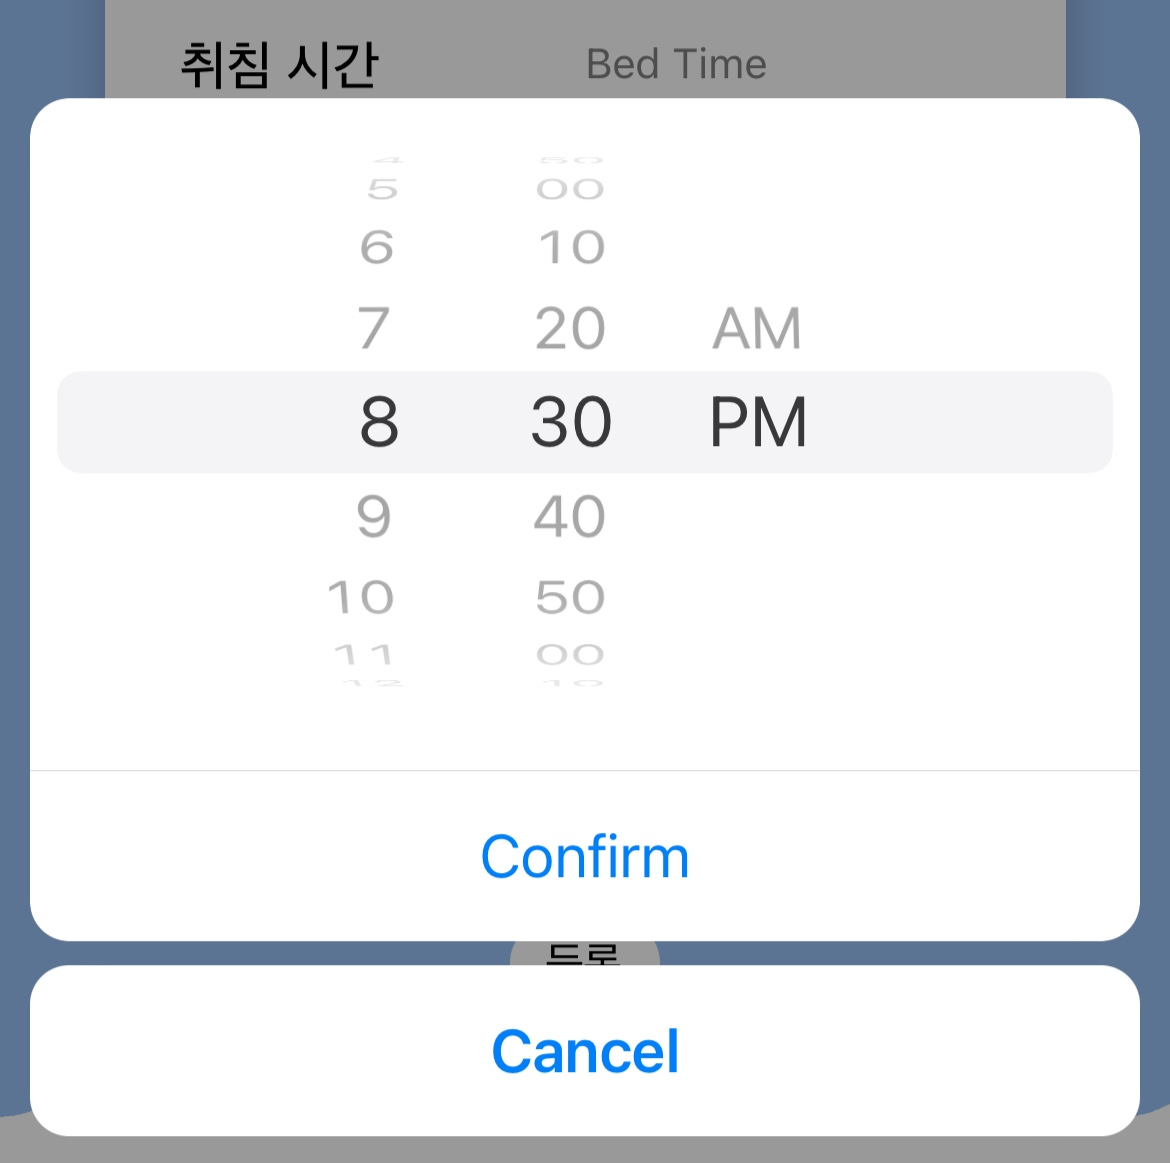
\includegraphics[width=3cm]{image/bed time.jpg}
\centering
\caption{Bed time / Wakeup time}
\label{fig:Bed time}
\end{figure}

\par \begin{figure}[h!]
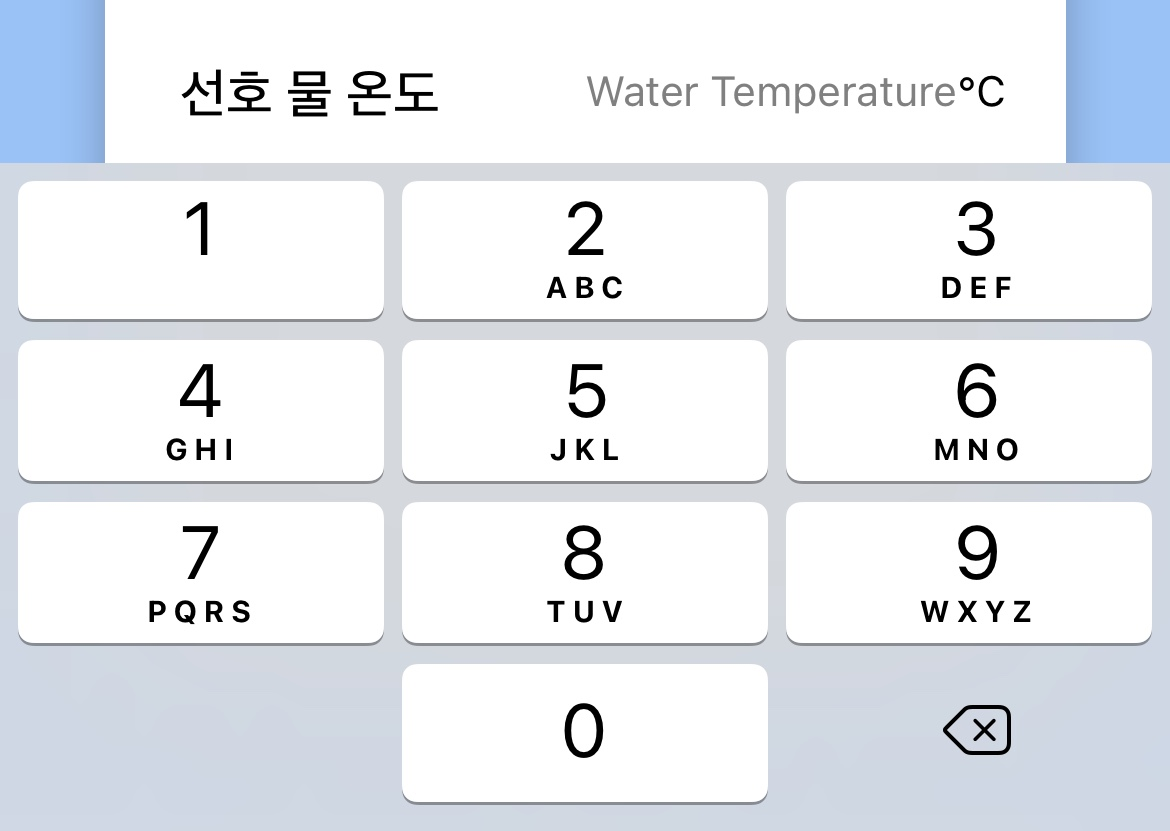
\includegraphics[width=3cm]{image/temperature.jpg}
\centering
\caption{Preffered temperature}
\label{fig:Preffered temperature}
\end{figure}

[Fig. \ref{fig:regiPerson}] Information needed to add human member include nickname, weight, wake-up/bed time, preferred water temperature, water intake goal, and water intake cycle. The field where the nickname can be entered can use letters and numbers. The user may determine a nickname of a combination of Korean, English, and numbers. Weight, preferred water temperature, and water intake goal are provided in fields where only numbers can be entered [Fig. \ref{fig:Preffered temperature}]. All of these values are allowed only the integer value. The wake-up/bed time and the water intake cycle are provided in a form in which values can be selected so that users can select values [Fig. \ref{fig:Bed time}]. The personal information of the input person is stored in the DANBI database. Based on the entered physiological information, the recommended amount of water intake and the recommended cycle of water intake are provided. The recommended amount of water intake is calculated as [weight (kg) * 30(ml)].\cite{waterIntake_Human} The recommended amount and recommended cycle of water intake can be changed by the user, and when it is confirmed, the amount of water intake is automatically calculated and provided to the user.
\item Pet

\par \begin{figure}[h!]
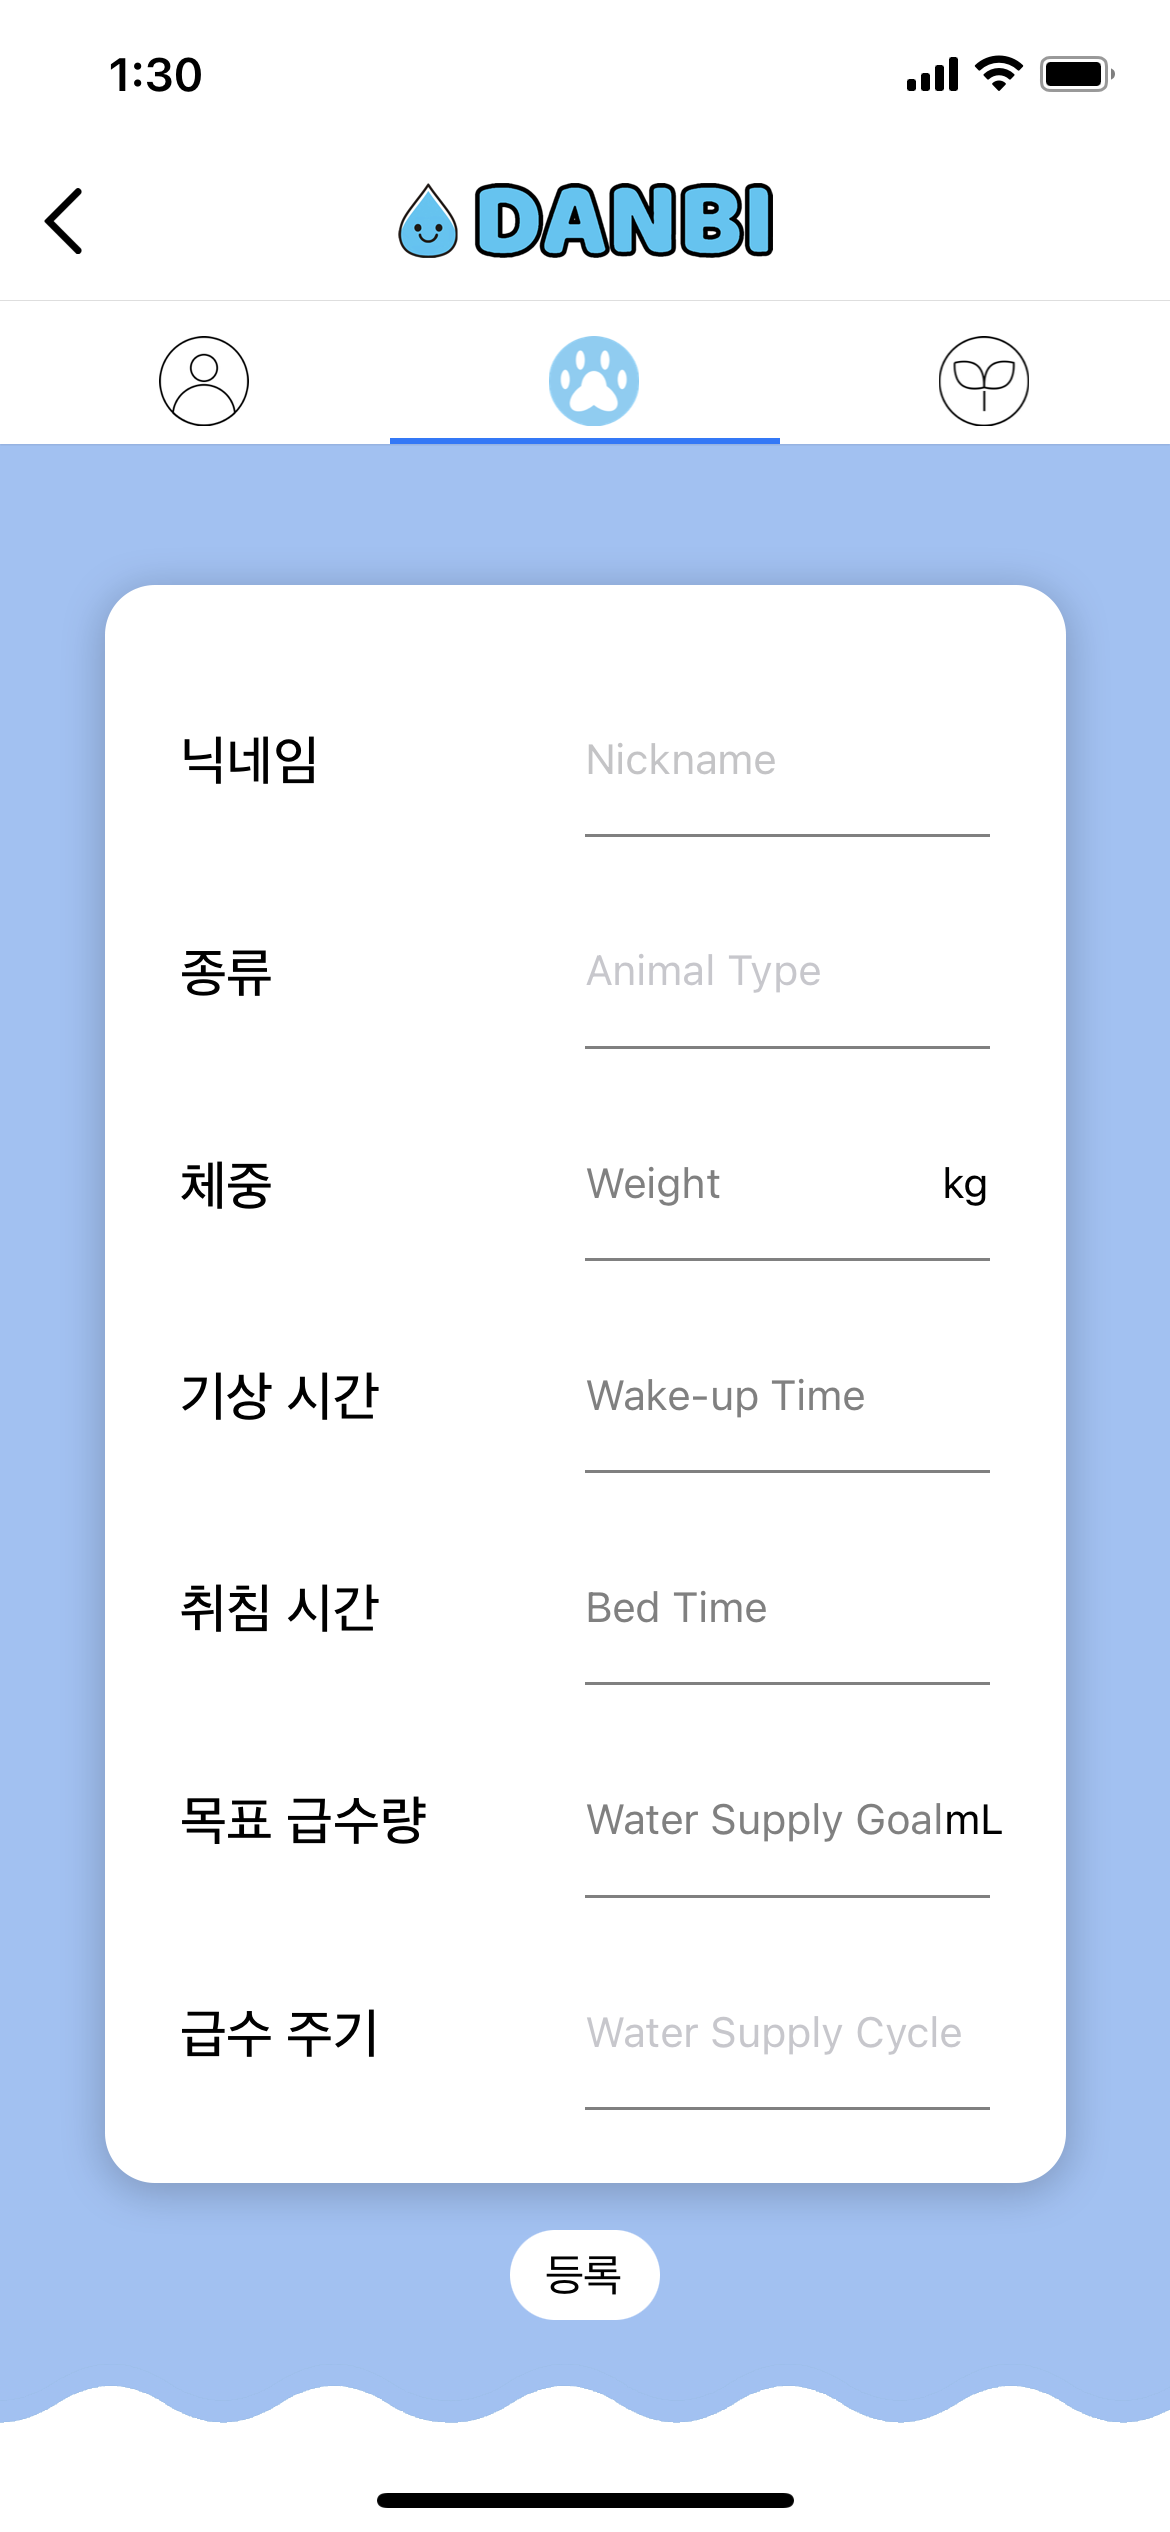
\includegraphics[width=3cm]{page/regiPet.png}
\centering
\caption{Registration\_Pet}
\label{fig:regiPet}
\end{figure}

[Fig. \ref{fig:regiPet}] Information needed to add animal members includes nicknames, animal type (dogs/cats), weight, wake-up/bed time, water supply goal, and water supply cycle. The nicknames of animal members are also allowed to use letters and numbers. Animal types are provided in the form of a selection box that can be selected between dogs and cats. Weight and water supply goal are provided as fields where only numbers can be entered, and only integer values are allowed. The wake-up/bed time and water intake cycle are provided in a form in which values can be selected, just like human members. The reason for receiving wake-up/bed time to register animal members is that the time to supply water to animals must be calculated and provided according to human activity time. The input animal information is stored in the DANBI database. Based on the species and weight of the input animal, the recommended amount and recommended cycle of water intake are calculated and provided.\cite{waterIntake_Pet}

- Dog with a weight of 10kg or less : recommended amount of water supply is calculated as [ weight(kg) * 60(ml) ]

- Dog with a weight 11kg to 25 kg : recommended amount of water supply is calculated as [ weight(kg) * 50(ml) ]

- Dog with a weight 26kg or more : recommended amount of water supply is calculated as [ weight(kg) * 40(ml) ]

- Cat : recommended amount of water supply is calculated as [ weight(kg) * 45(ml) ]

The recommended amount and cycle of water supply can be changed according to the characteristics of the animals observed by the user, and when it confirmed, the amount of water supply is automatically calculated and provided to the user. The user can manage the water supply of pet accordingly.
\item Plant

\par \begin{figure}[h!]
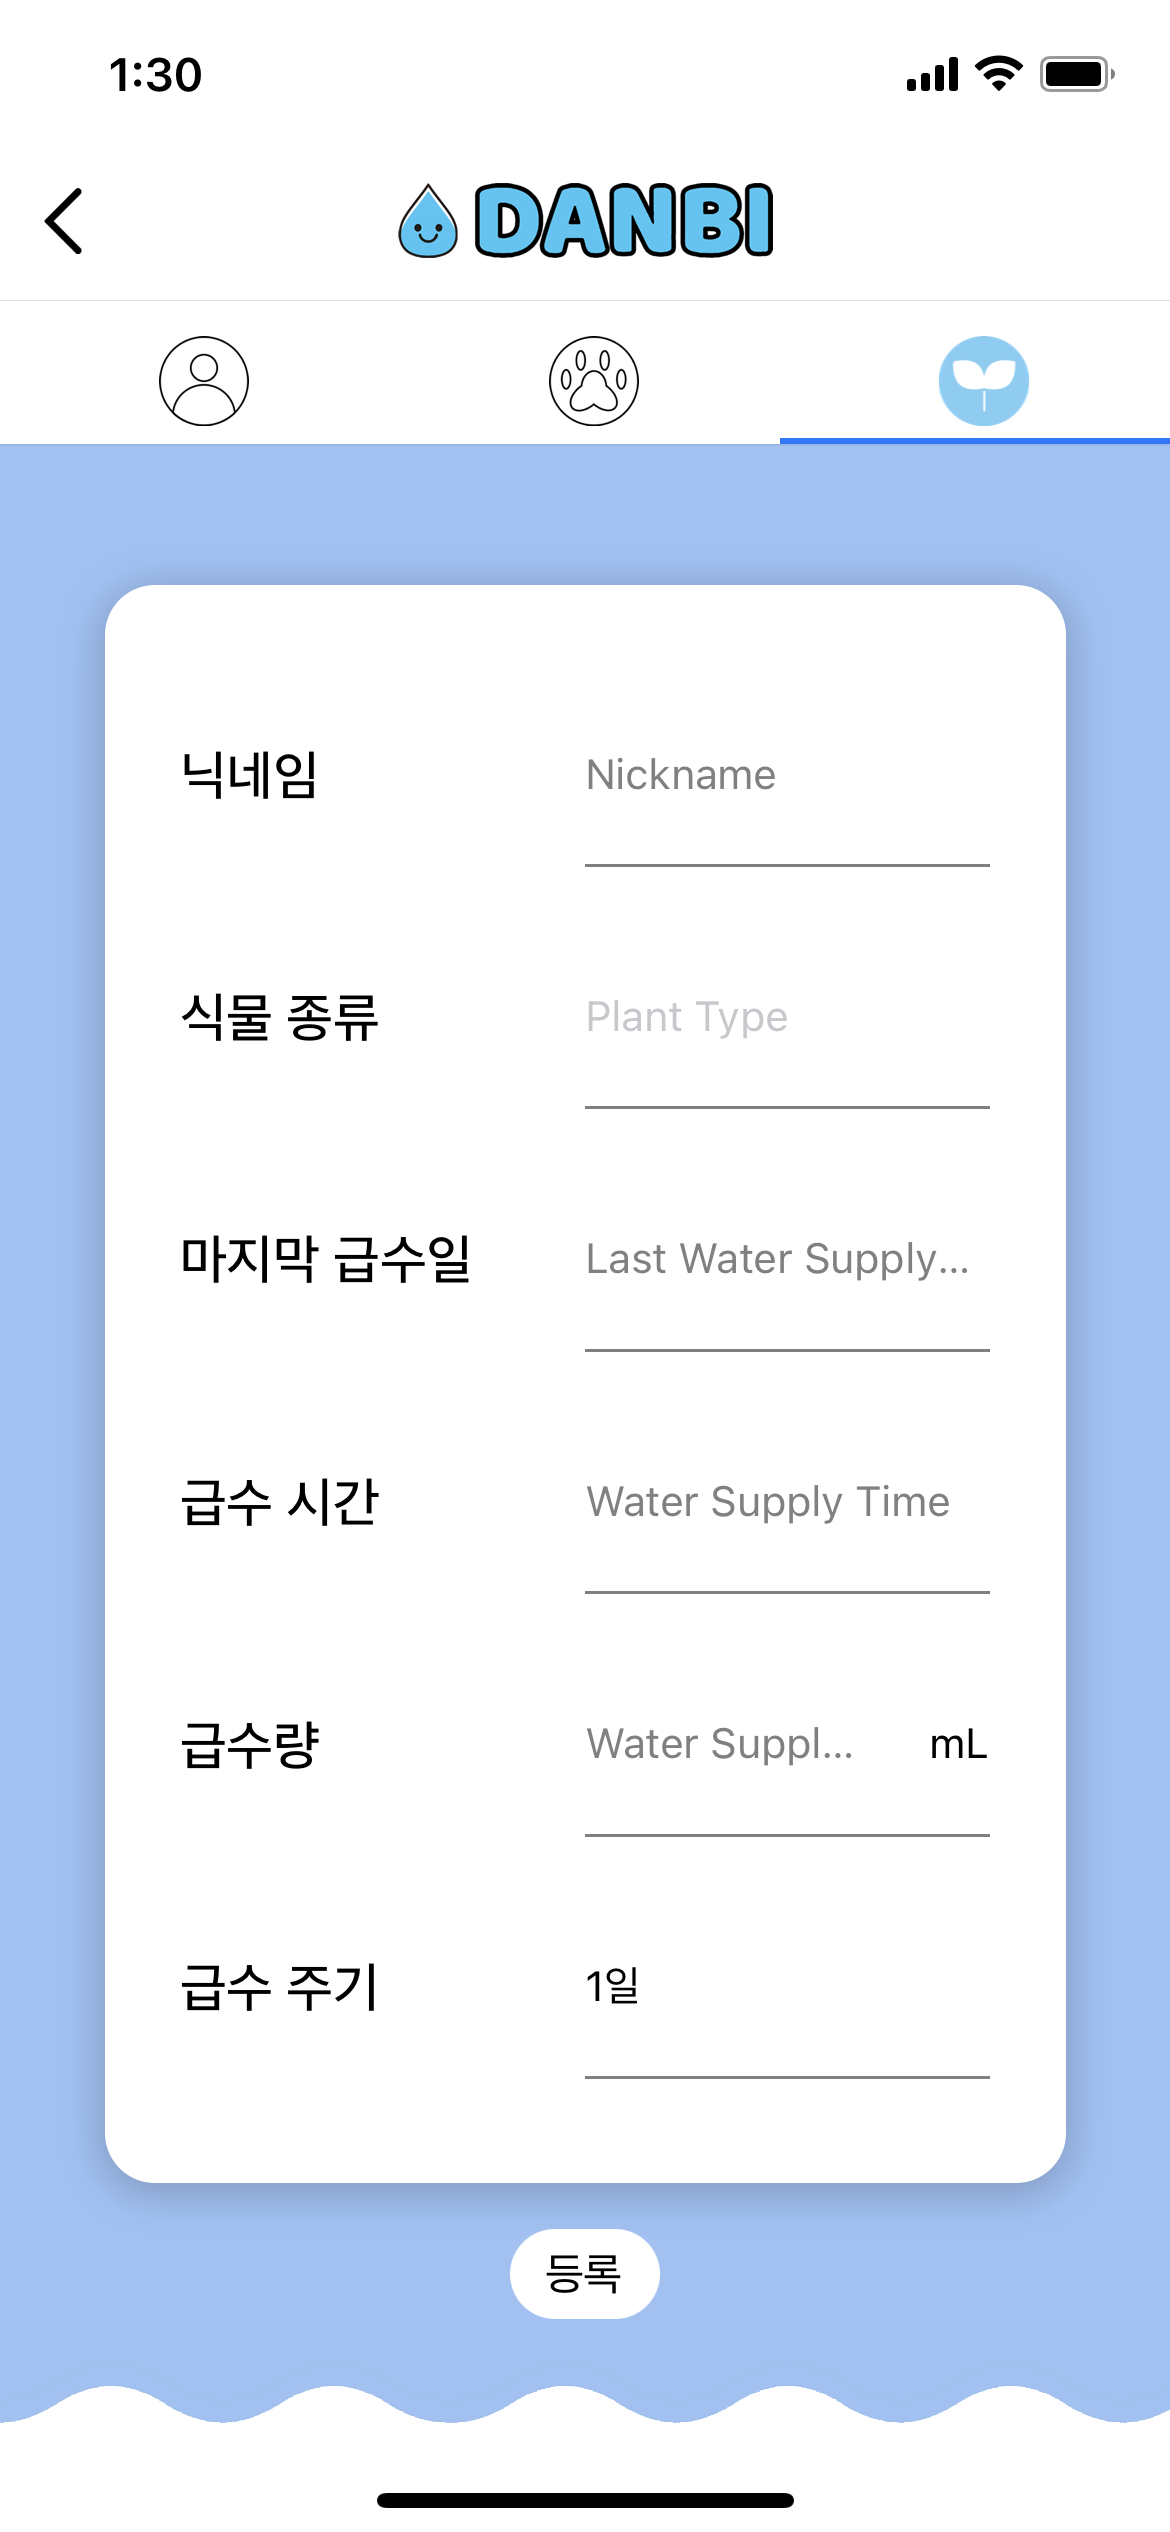
\includegraphics[width=3cm]{page/regiPlant.png}
\centering
\caption{Registration\_Plant}
\label{fig:regiPlant}
\end{figure}

\par \begin{figure}[h!]
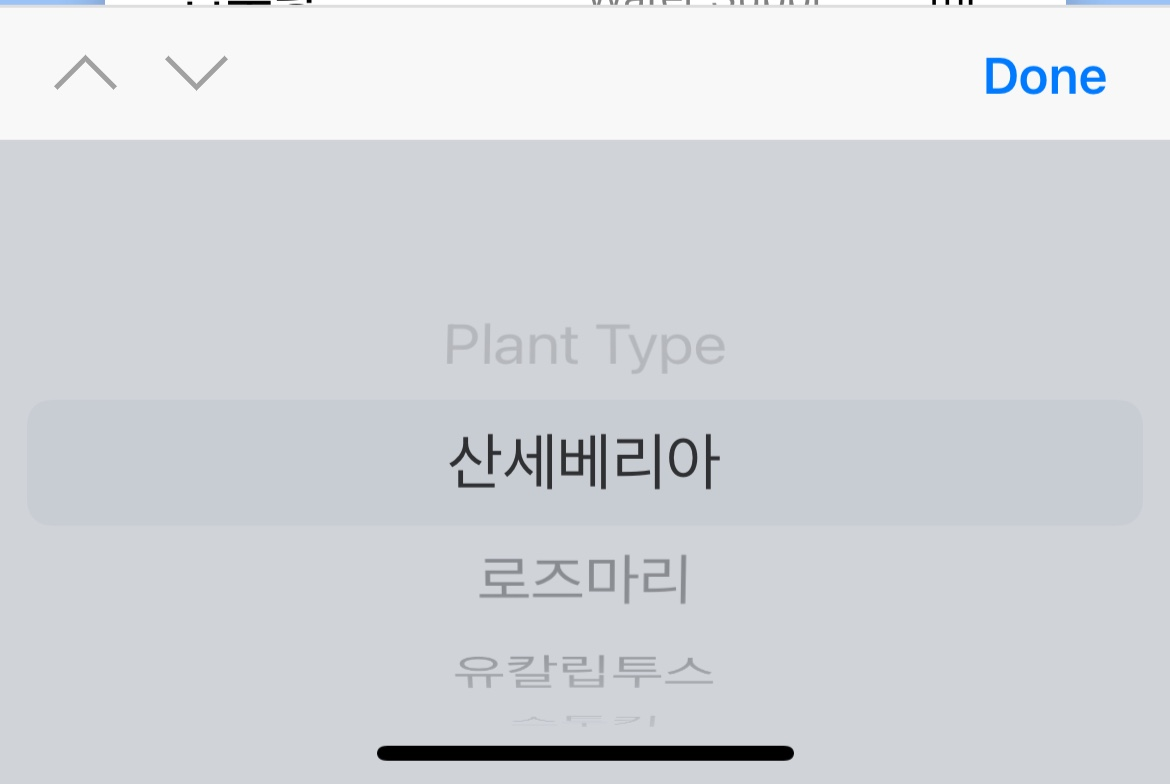
\includegraphics[width=3cm]{image/Plant type.jpg}
\centering
\caption{Plant type}
\label{fig:type}
\end{figure}

\par \begin{figure}[h!]
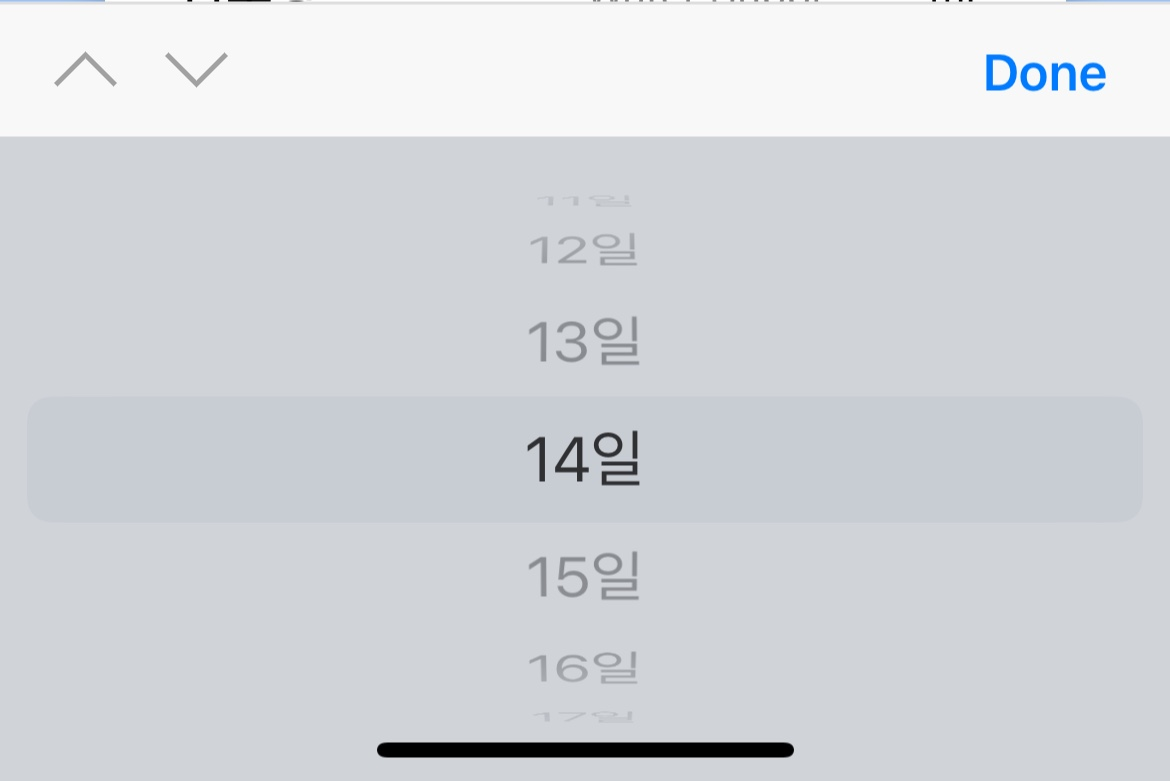
\includegraphics[width=3cm]{image/plant cycle.jpg}
\centering
\caption{Plant cycle}
\label{fig:plant cycle}
\end{figure}

\par \begin{figure}[h!]
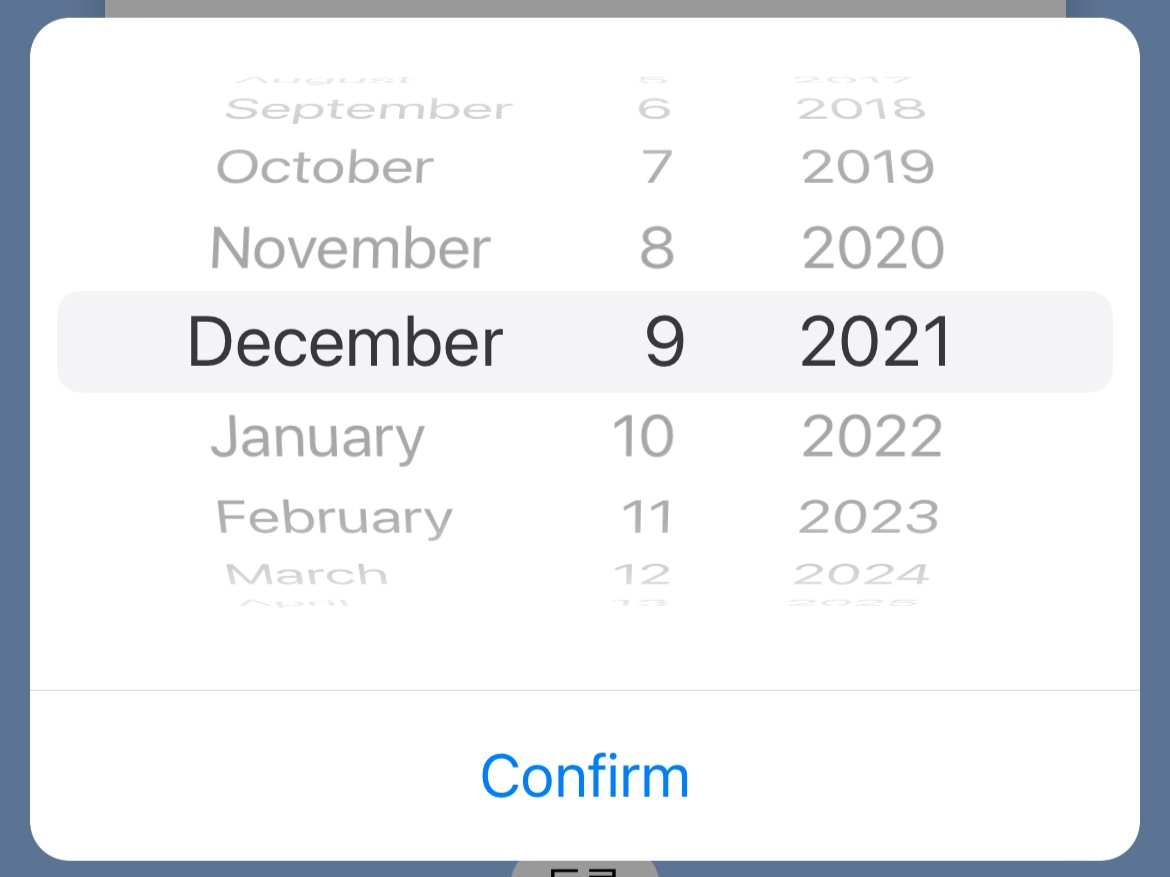
\includegraphics[width=3cm]{image/date.jpg}
\centering
\caption{Date}
\label{fig:date}
\end{figure}

[Fig. \ref{fig:regiPlant}] Information required when adding plant member include nickname, plant type, last water supply date, water supply time, water supply amount at once, and water supply cycle. Nickname information may also be input with characters and numbers. When adding plant members, DANBI basically provides popular plant species. The user can find and select a plant species to be registered among the species provided. [Fig. \ref{fig:type}] If it does not exist in the built-in plant, the user can add it. It automatically provides a recommended water supply cycle according to the input plant species.\cite{waterIntake_Plant} This can be changed by the user. [Fig. \ref{fig:plant cycle}] The water supply recommendation cycle is provided as a selection box and can be changed by selecting another value. The last water supply date is required to calculate the next water supply date. The date is provided to the select box [Fig. \ref{fig:date}], and the user can select a date. The water supply time is provided in a select box where the time can be selected. Plants have a long water supply cycle, so when the water supply date arrives, a notification is sent according to the time selected by the user. In the case of the recommended amount of water supply, the user inputs it directly because it depends on the size of the plant. The recommended amount of water field can only be entered by numbers, and only the integer value is allowed.
\end{enumerate}
\item \textbf{Member Specification page}

\par \begin{figure}[h!]
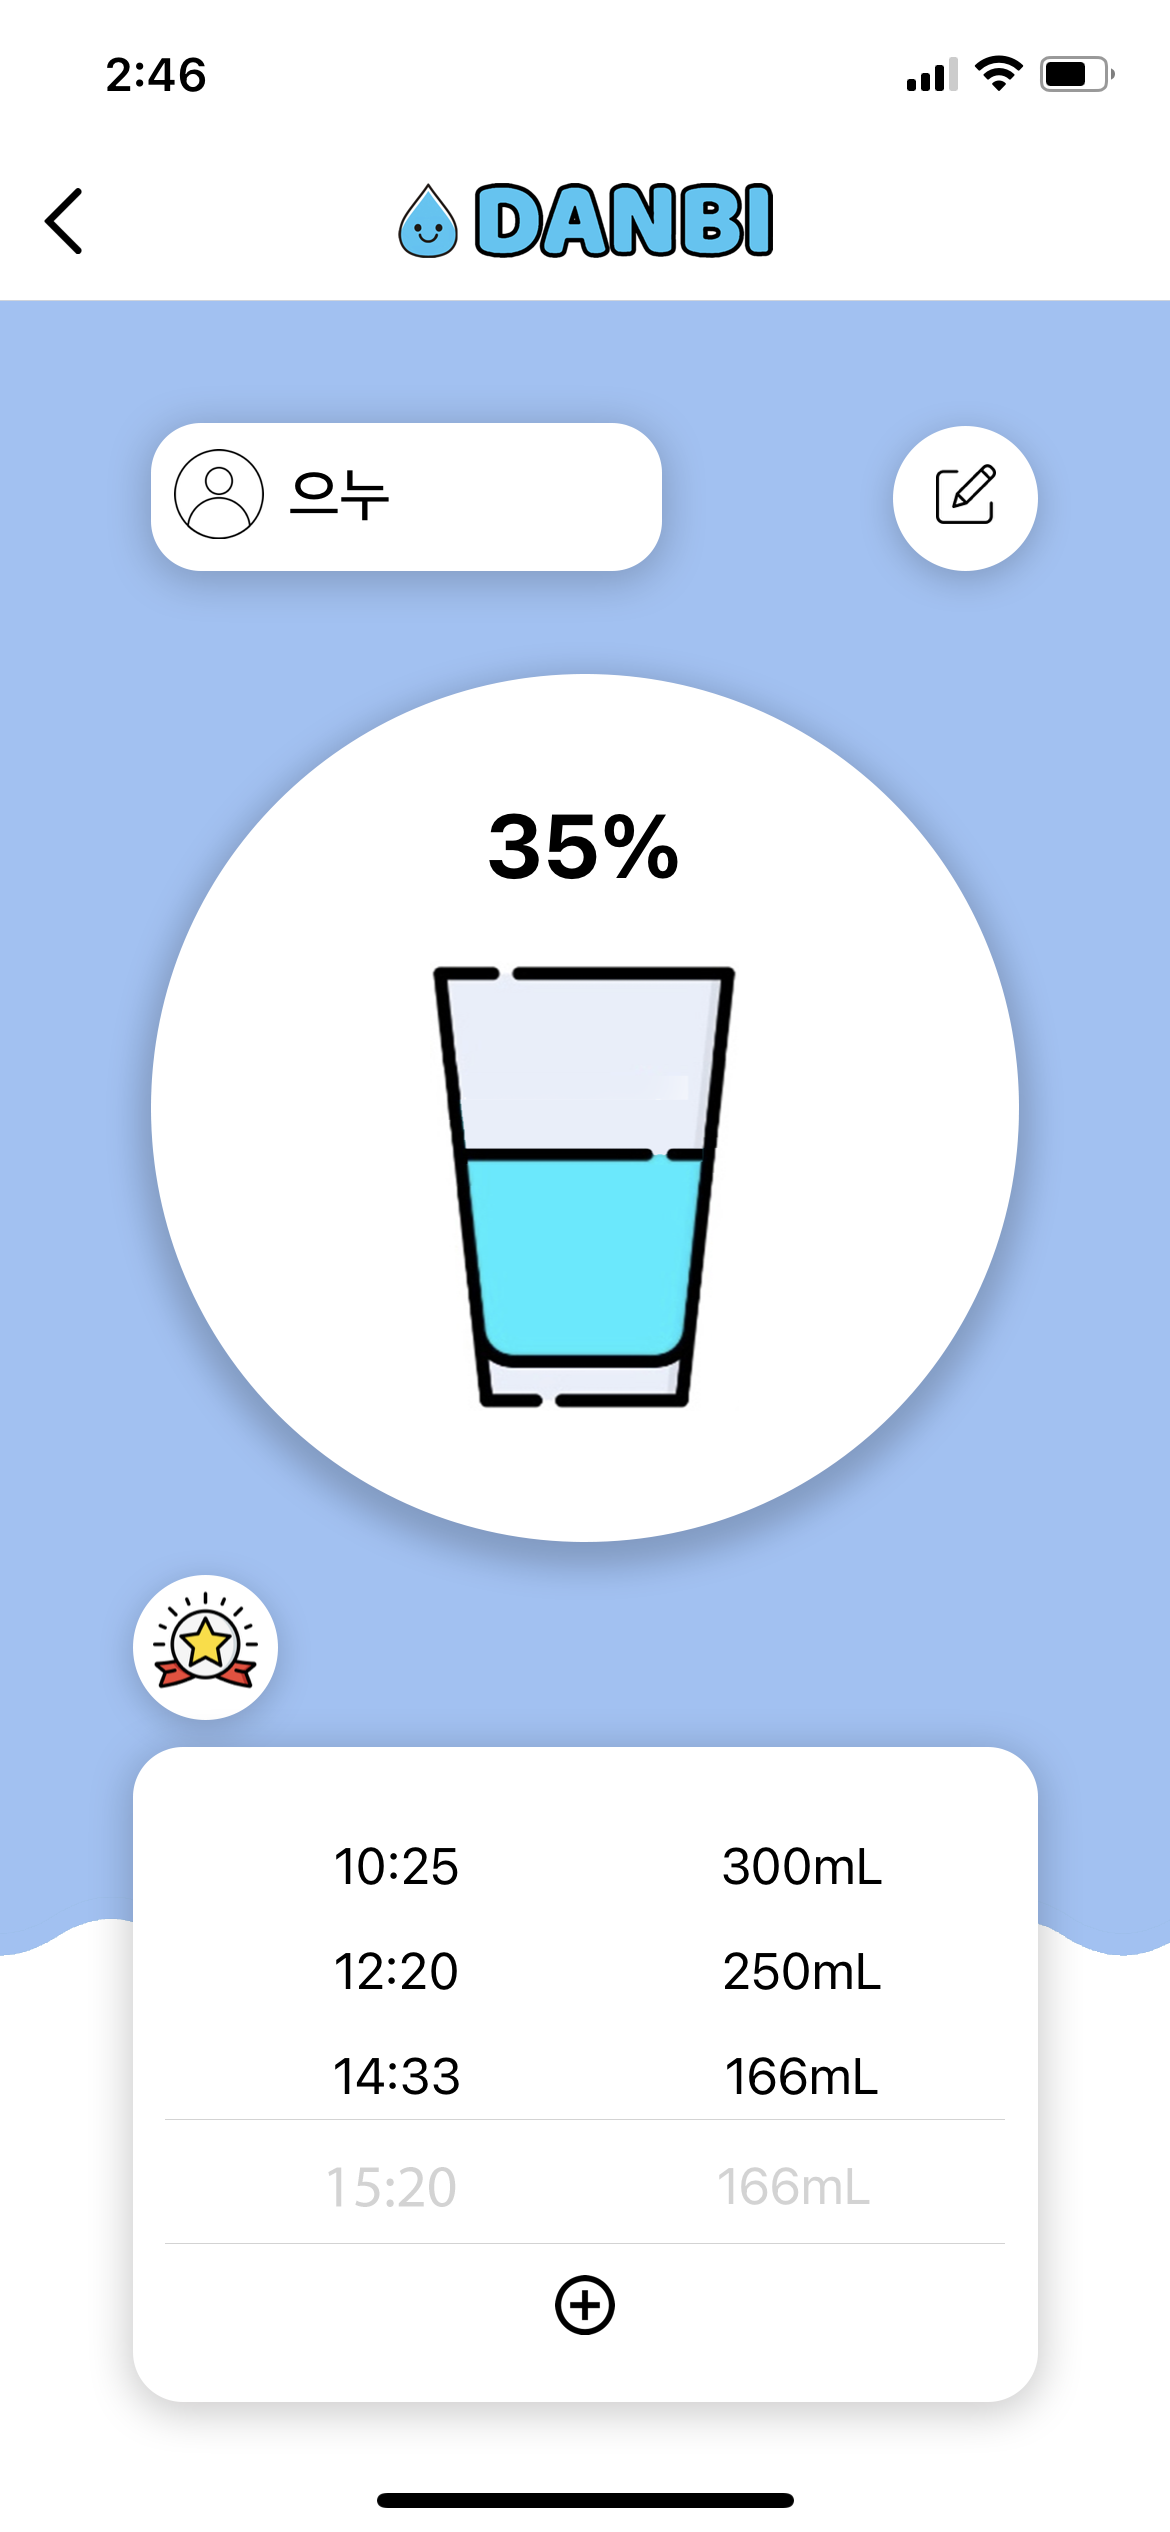
\includegraphics[width=3cm]{page/specificPerson.png}
\centering
\caption{Specification}
\label{fig:specPerson}
\end{figure}

[Fig. \ref{fig:specPerson}] If user click a specific member in the 'Main page', user can access the 'Member Specification page' of the corresponding member. The 'Member Specification Page' provides data that visually analyzes the water intake information of a member. Specific information provided includes 'Today's achievement', 'Water Record', 'Award Stamp'. By comparing the amount of water intake goal for today with the actual intake, it provides a picture of a water glass filling up. It also provides percentage information by calculating the achievement rate. At the bottom of the page, the time of drinking water during the day is organized and provided as a table. By pressing the black '+' button below the table, additional information on water intake can be entered manually. In addition, the input information may be modified. Biological information and water intake settings can be changed, and the button is in the upper right corner. The water intake stamp can be checked by clicking the left middle stamp-shaped button. Pressing this button provides a calendar, and the calendar is circled in sky blue on the day when water intake is achieved.

\begin{enumerate}
\setlength{\parindent}{2ex}
\item Today's Achievement

\par \begin{figure}[h!]
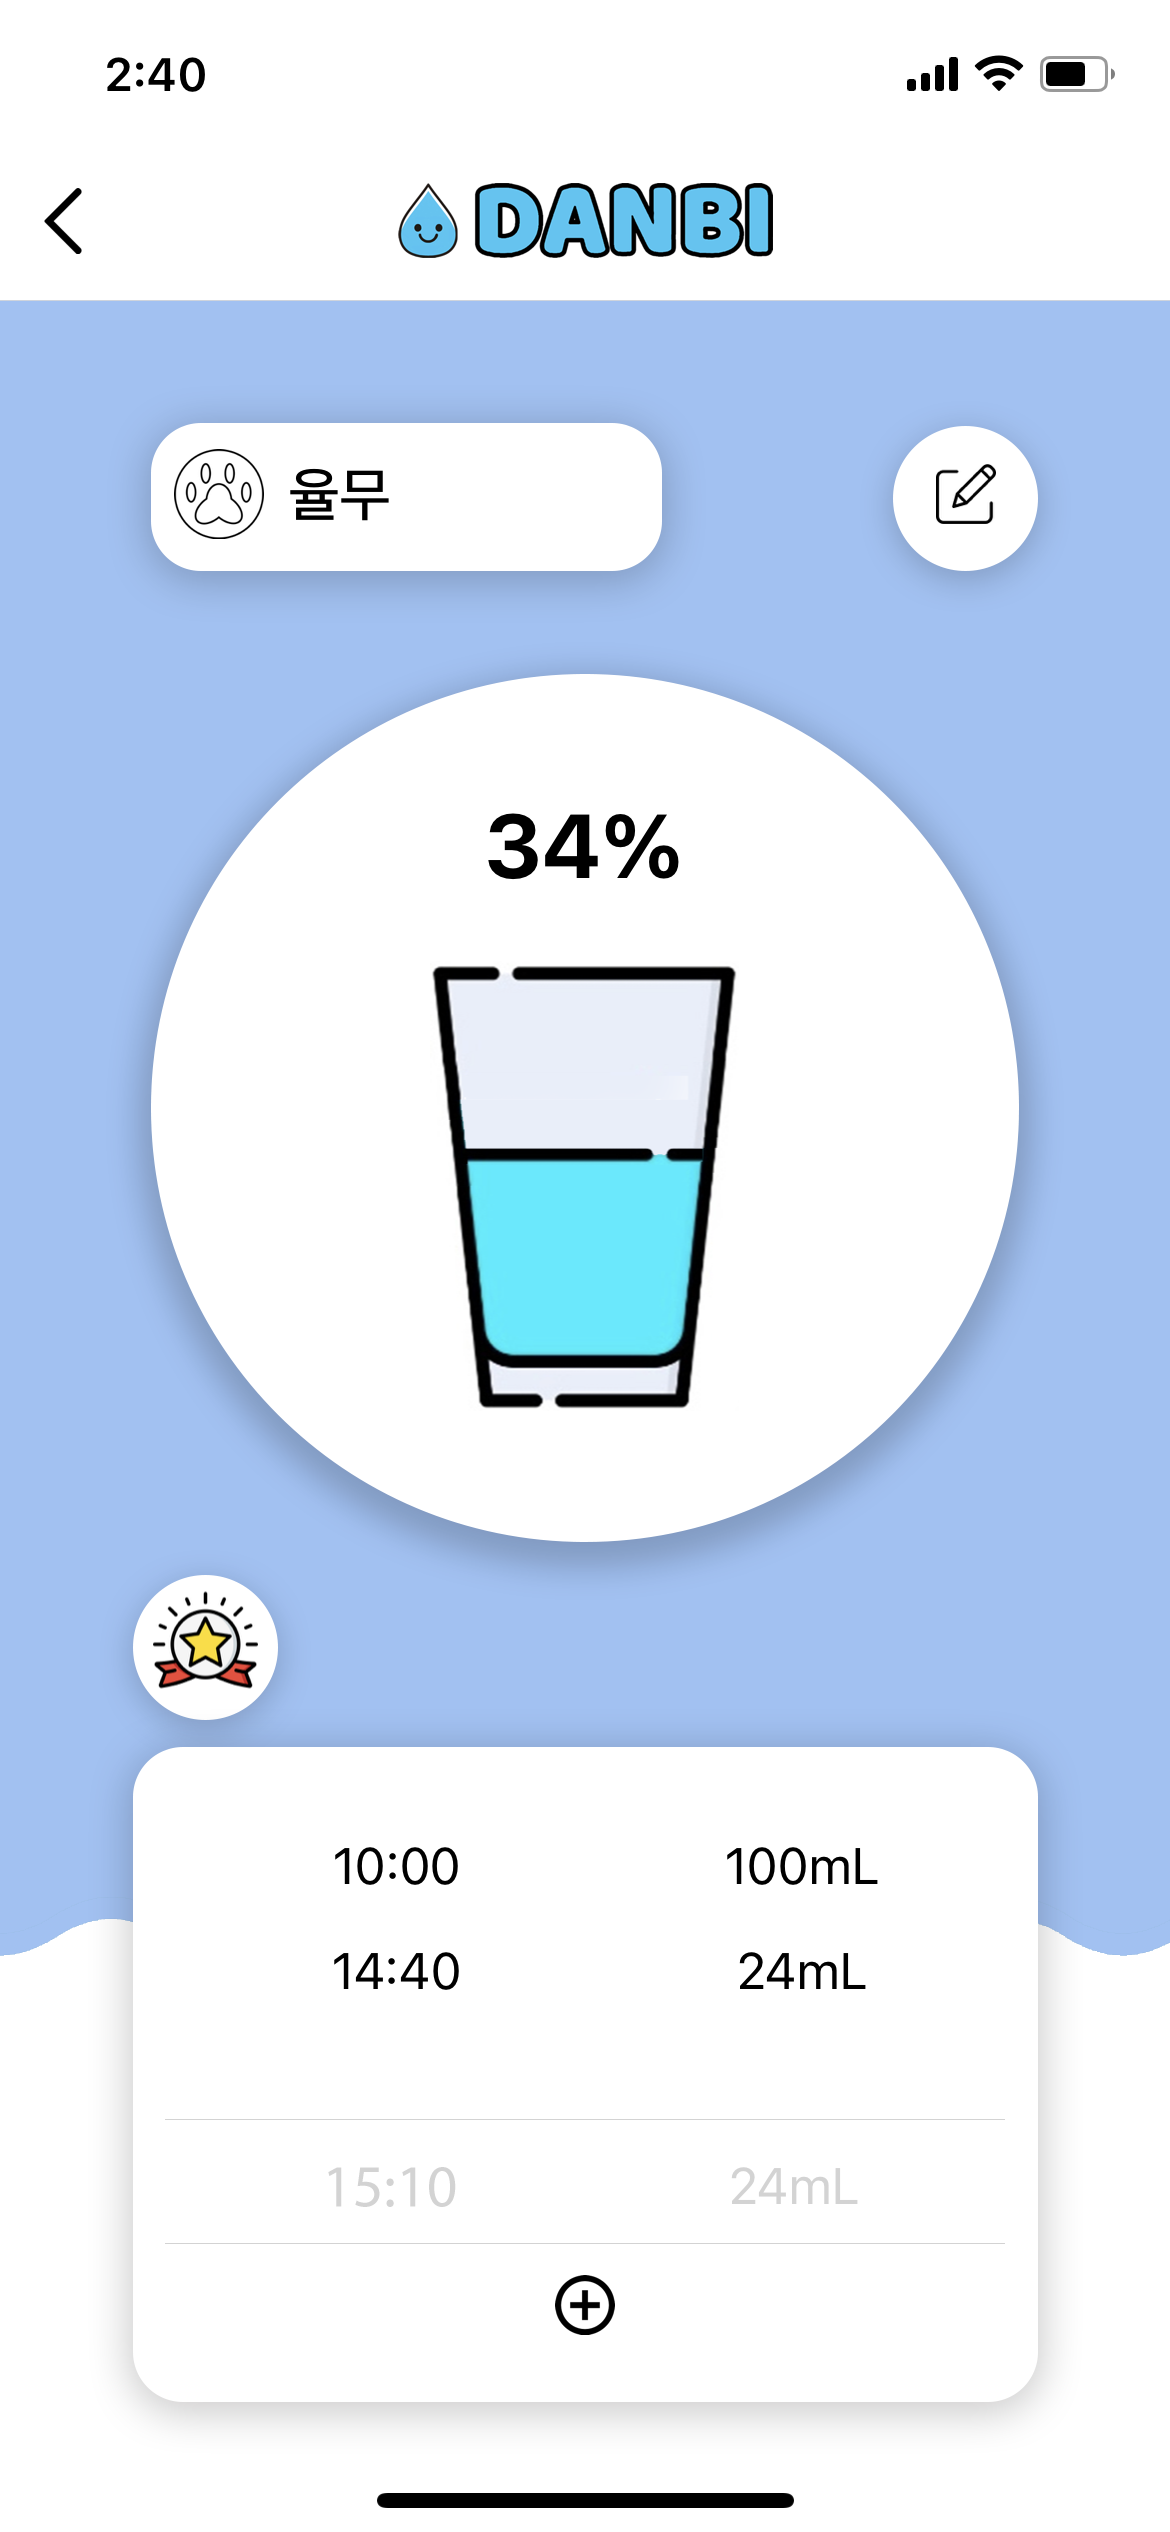
\includegraphics[width=3cm]{page/specificPet.png}
\centering
\caption{Today's achievement}
\label{fig:specPet}
\end{figure}


[Fig. \ref{fig:specPet}] It visually represents and provides the member's daily water intake achievement. The water glass picture provides intuitive water intake achievement by filling the water according to the degree of water intake of the member. The graph is made based on information on the daily water intake and the daily water intake goal stored in the database. User can visually check their daily water intake and the remaining intake at a glance by receiving a visual indication of how much water intake today is compared to their daily intake goal and how much more to reach the goal.
\item Water Record

\par \begin{figure}[h!]
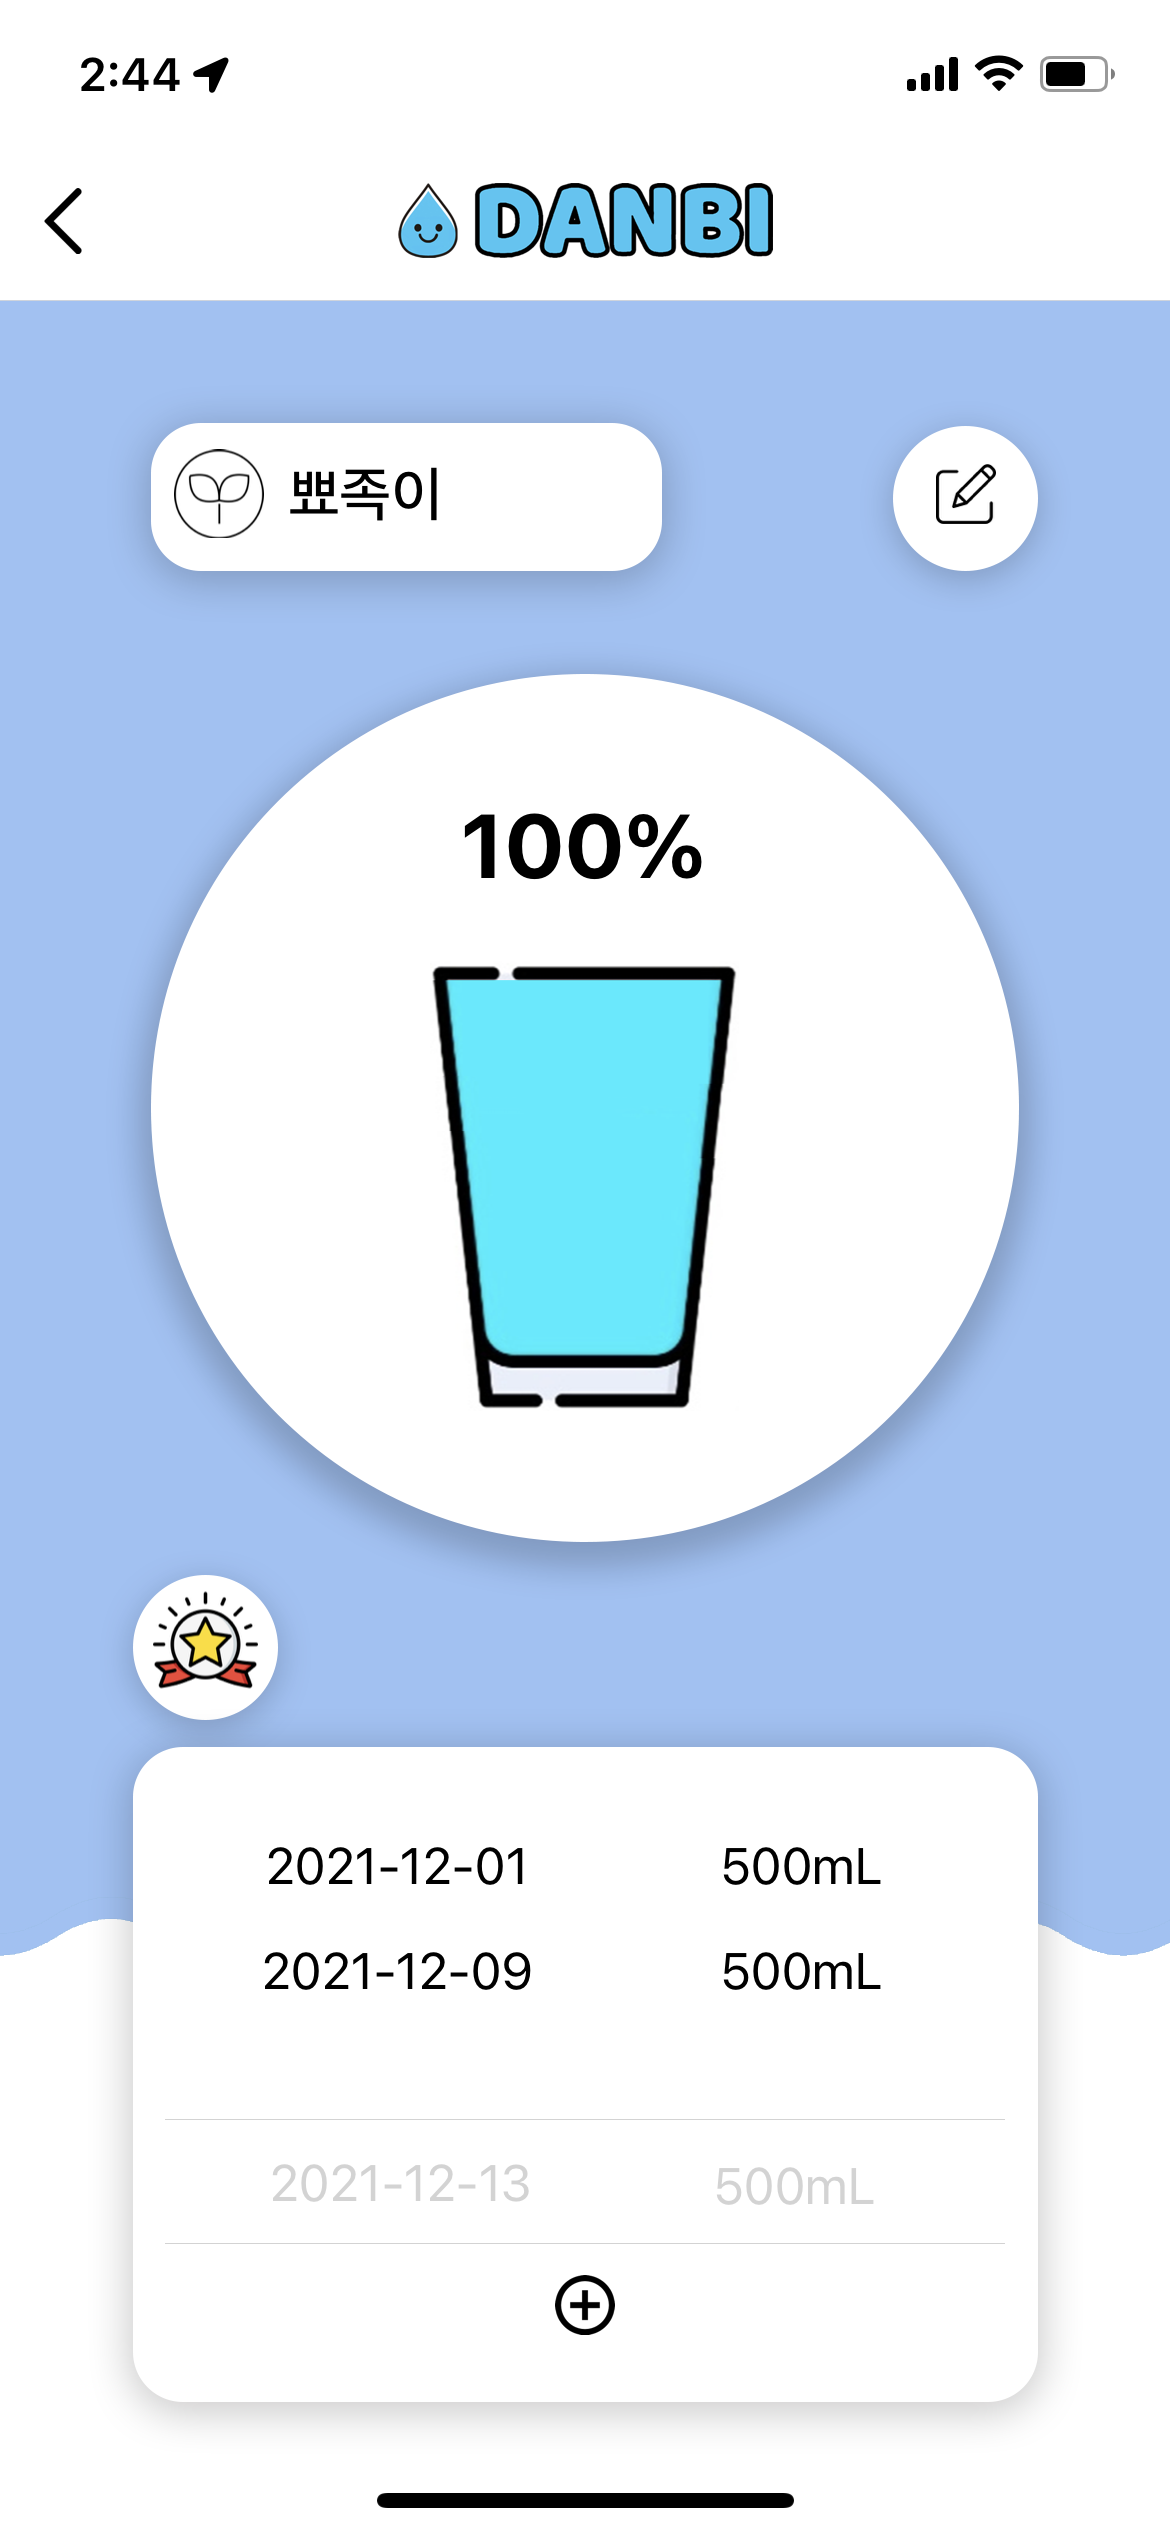
\includegraphics[width=3cm]{page/specificPlant.png}
\centering
\caption{Water Record}
\label{fig:specPlant}
\end{figure}

[Fig. \ref{fig:specPlant}] Specific intake information of members can be checked. It provides the time and amount of water consumed during the day. Below that, it provides the next estimated time to have water intake. On a daily basis, the time of water intake stored in the database and the amount of water intake at that time are transmitted to the server, and the application visualizes and provides it for user.
\item Add New Water Record

\par \begin{figure}[h!]
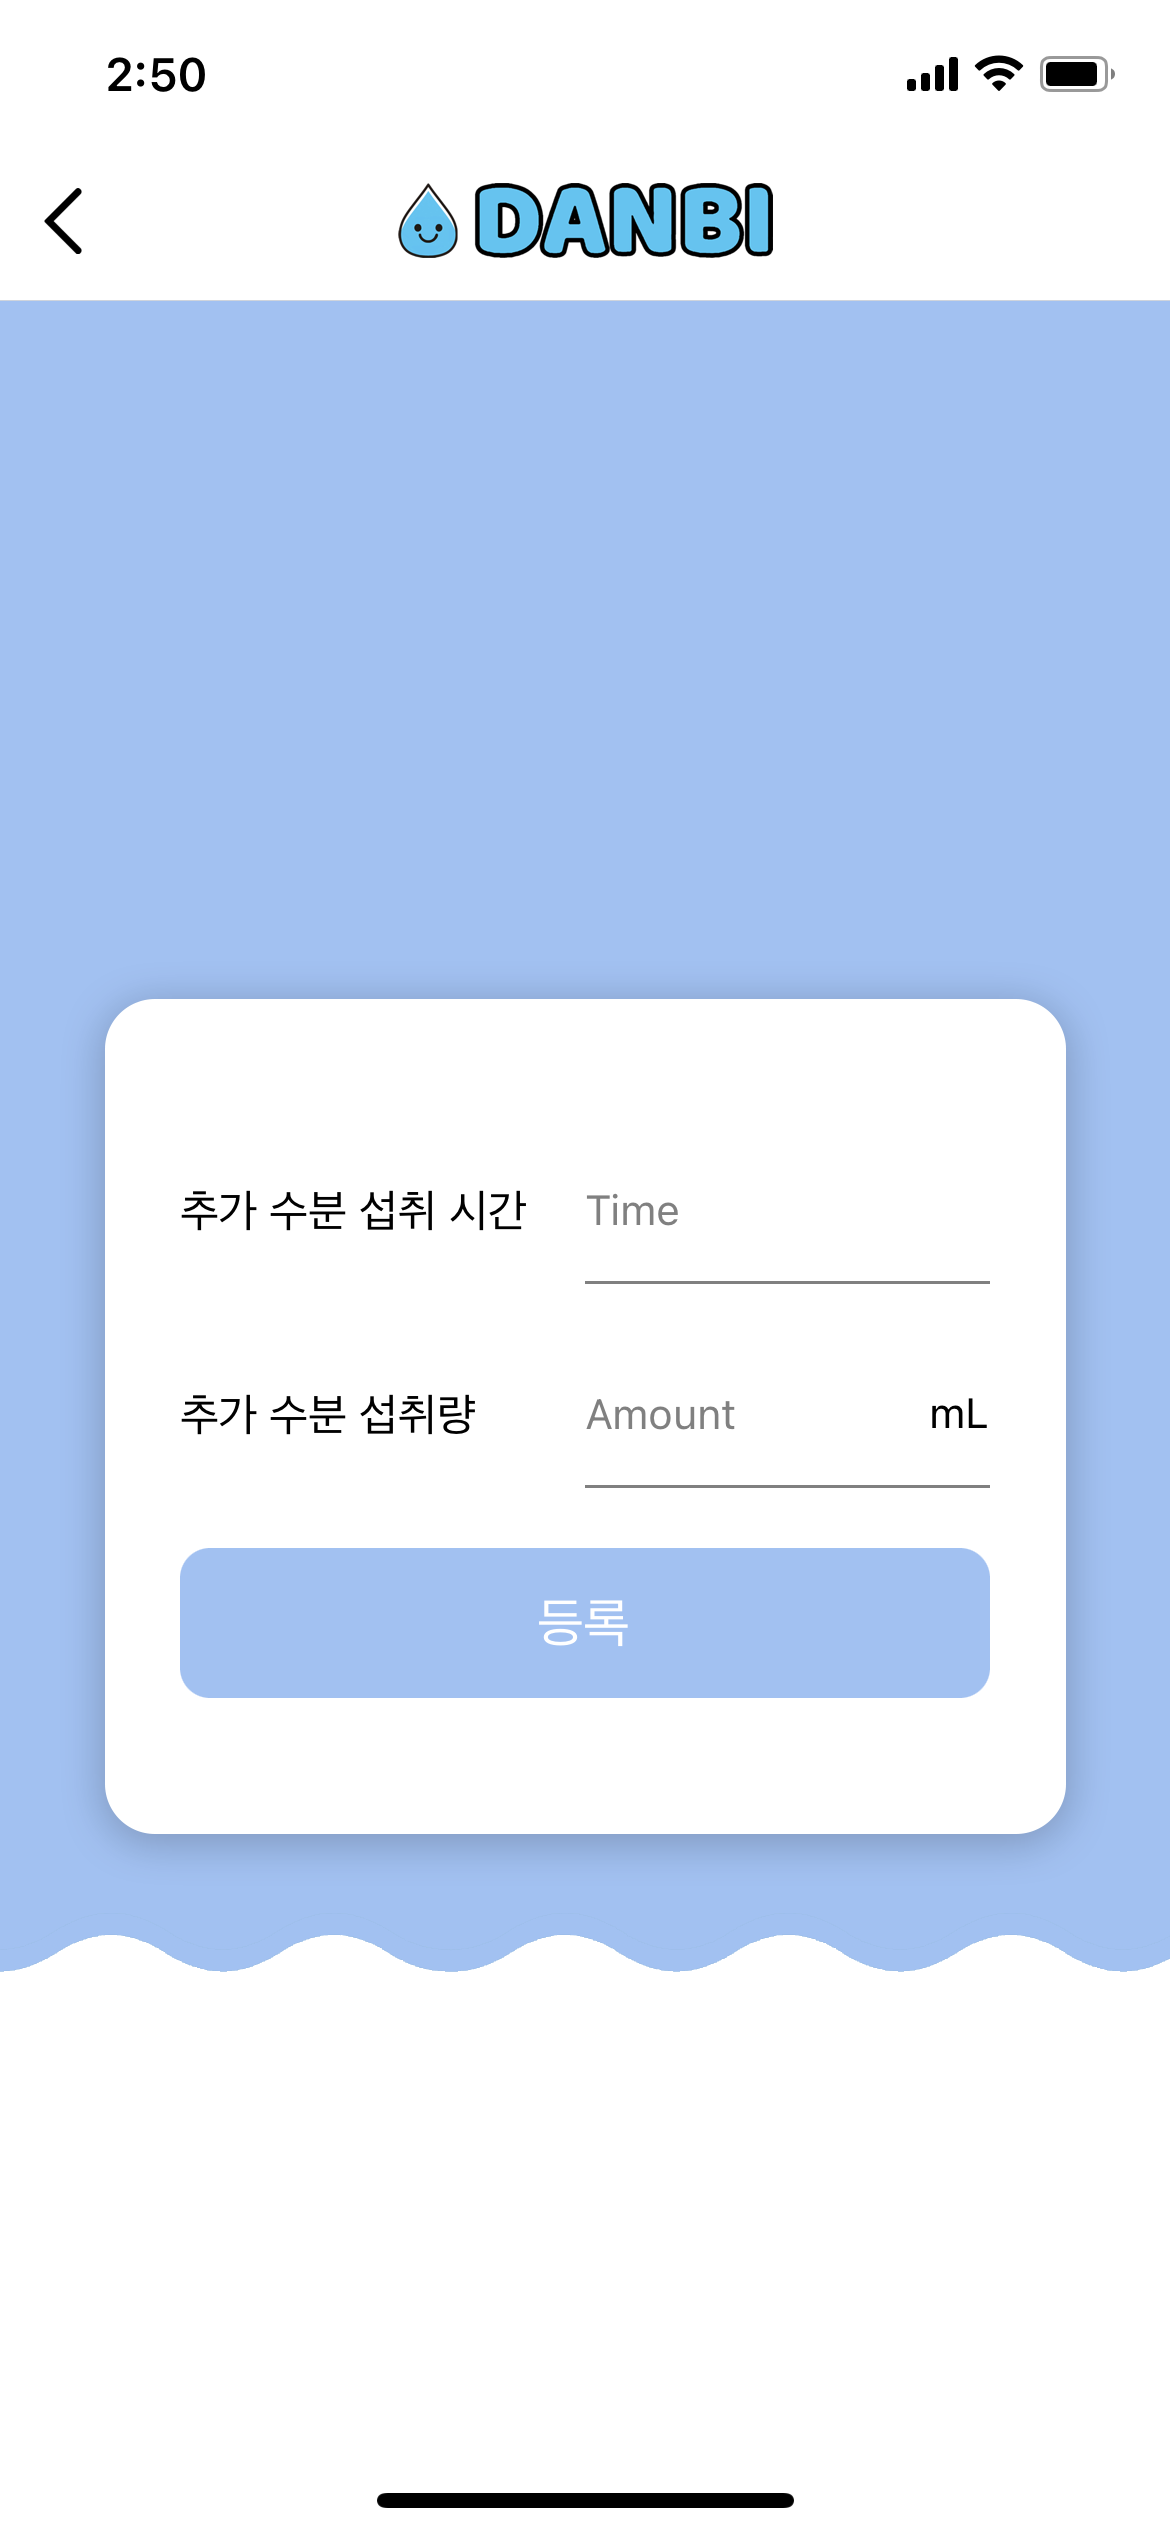
\includegraphics[width=3cm]{page/addWater.png}
\centering
\caption{Add water}
\label{fig:addWater}
\end{figure}

[Fig. \ref{fig:addWater}] The water intake information of the member may be manually input. In some cases, water intake information is not automatically recorded in the database, such as when drinking water other than pop up notification time or when a user pressed '미루기' to notification. In this case, the user manually inputs the time and amount of water intake to add data to the database. The 'Add New Water Record' page can be accessed through the black '+' button under the 'Water Record' table.
\item Edit Information

A page for changing information can be accessed through the edit icon in the upper right corner.

\par \begin{figure}[h!]
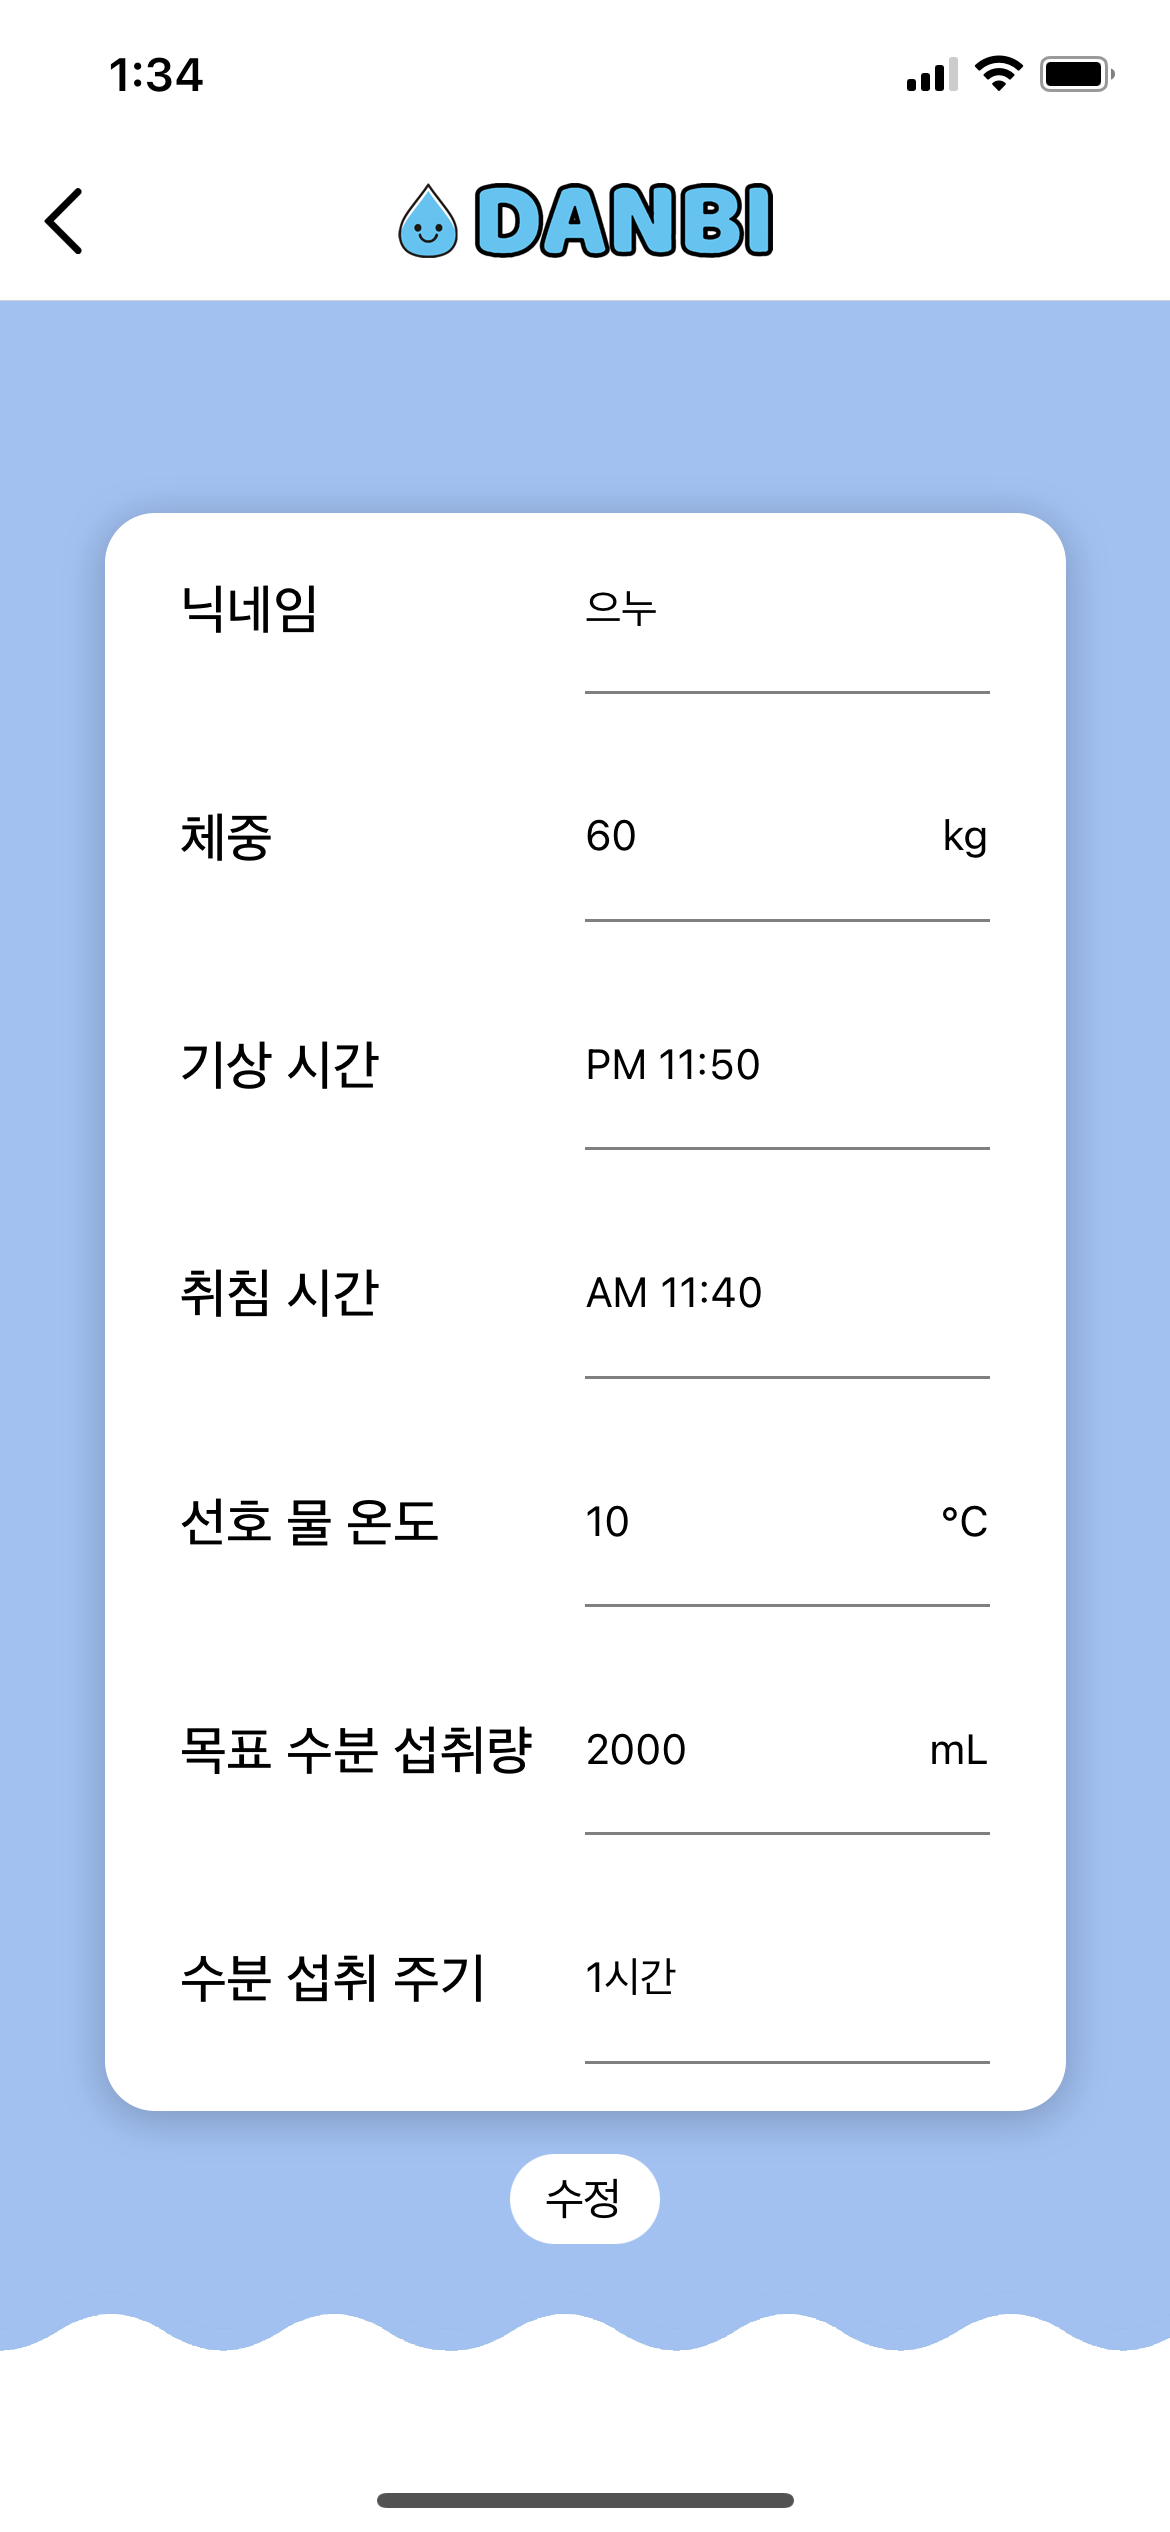
\includegraphics[width=3cm]{page/editPerson.png}
\centering
\caption{Edit\_Person}
\label{fig:editPerson}
\end{figure}

[Fig. \ref{fig:editPerson}] In the case of humans, the information edit page contains information on Nickname, Weight, Wake-up/bed time, Preferred water temperature, Water intake goal, and Water intake cycle, and it is same with when adding members. The user can change all values. Among them, modifying the weight value provides a new recommended daily water intake regardless of the previously set value, which can also be changed by the user.

\par \begin{figure}[h!]
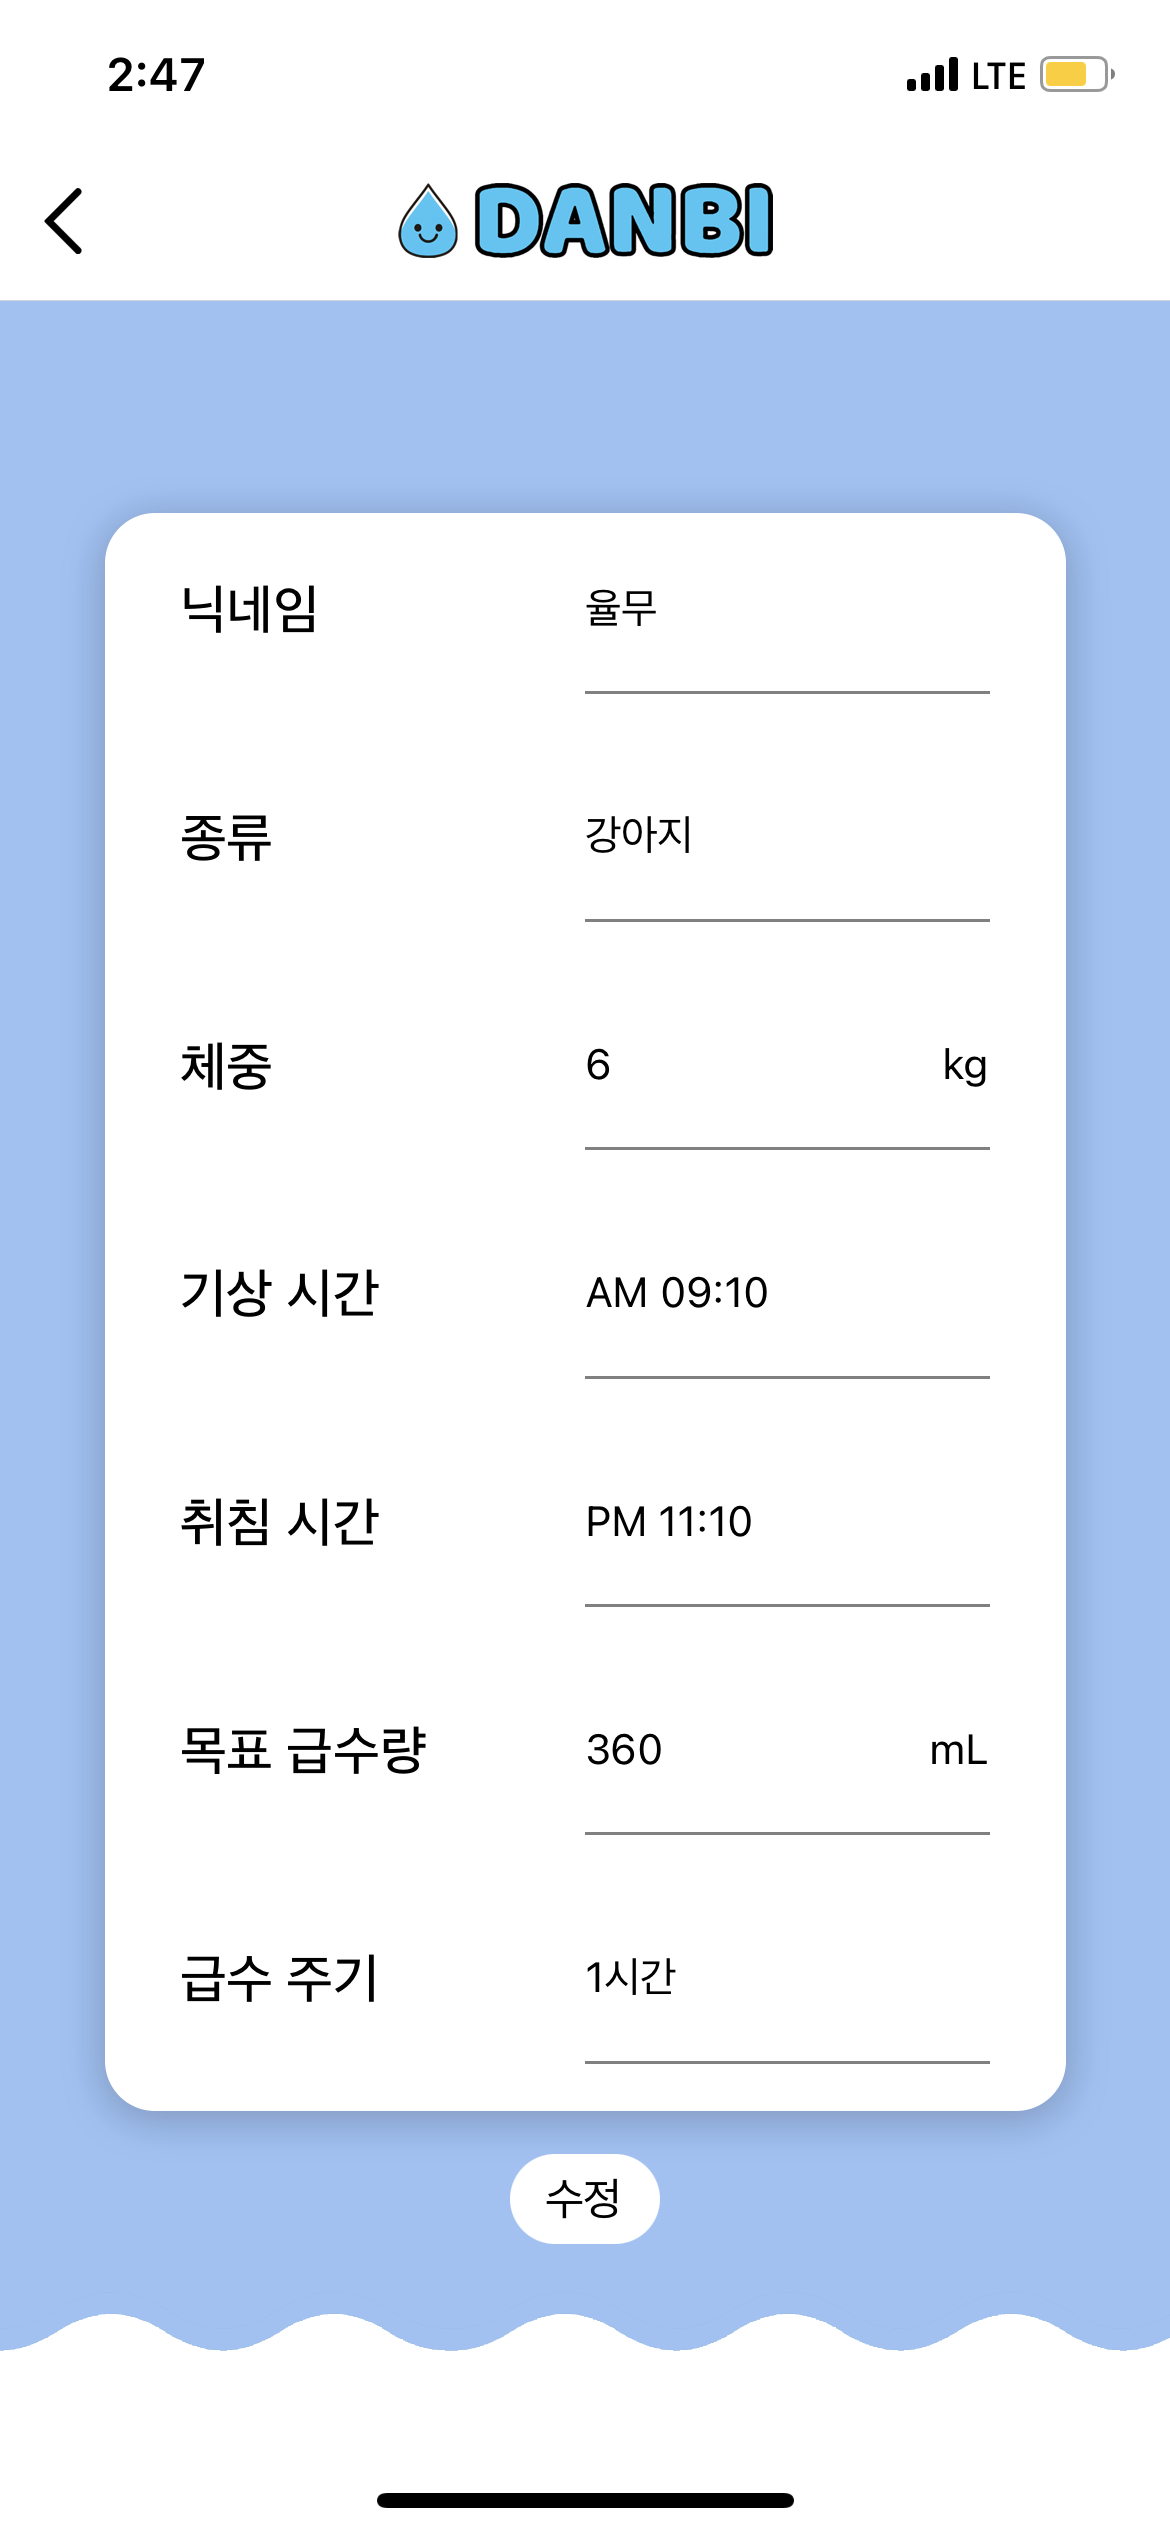
\includegraphics[width=3cm]{page/editPet.png}
\centering
\caption{Edit\_Pet}
\label{fig:editPet}
\end{figure}

[Fig. \ref{fig:editPet}] In the case of pets, the information edit page contains information on Nickname, Animal type(dog/cat), Weight, Wake-up/bed time, Water supply goal, Water supply cycle. All values except the type can be changed. Among them, when the weight value of the animal is edited, the recommended daily water intake and water supply cycle are recalculated and provided, which can be changed by the user.

\par \begin{figure}[h!]
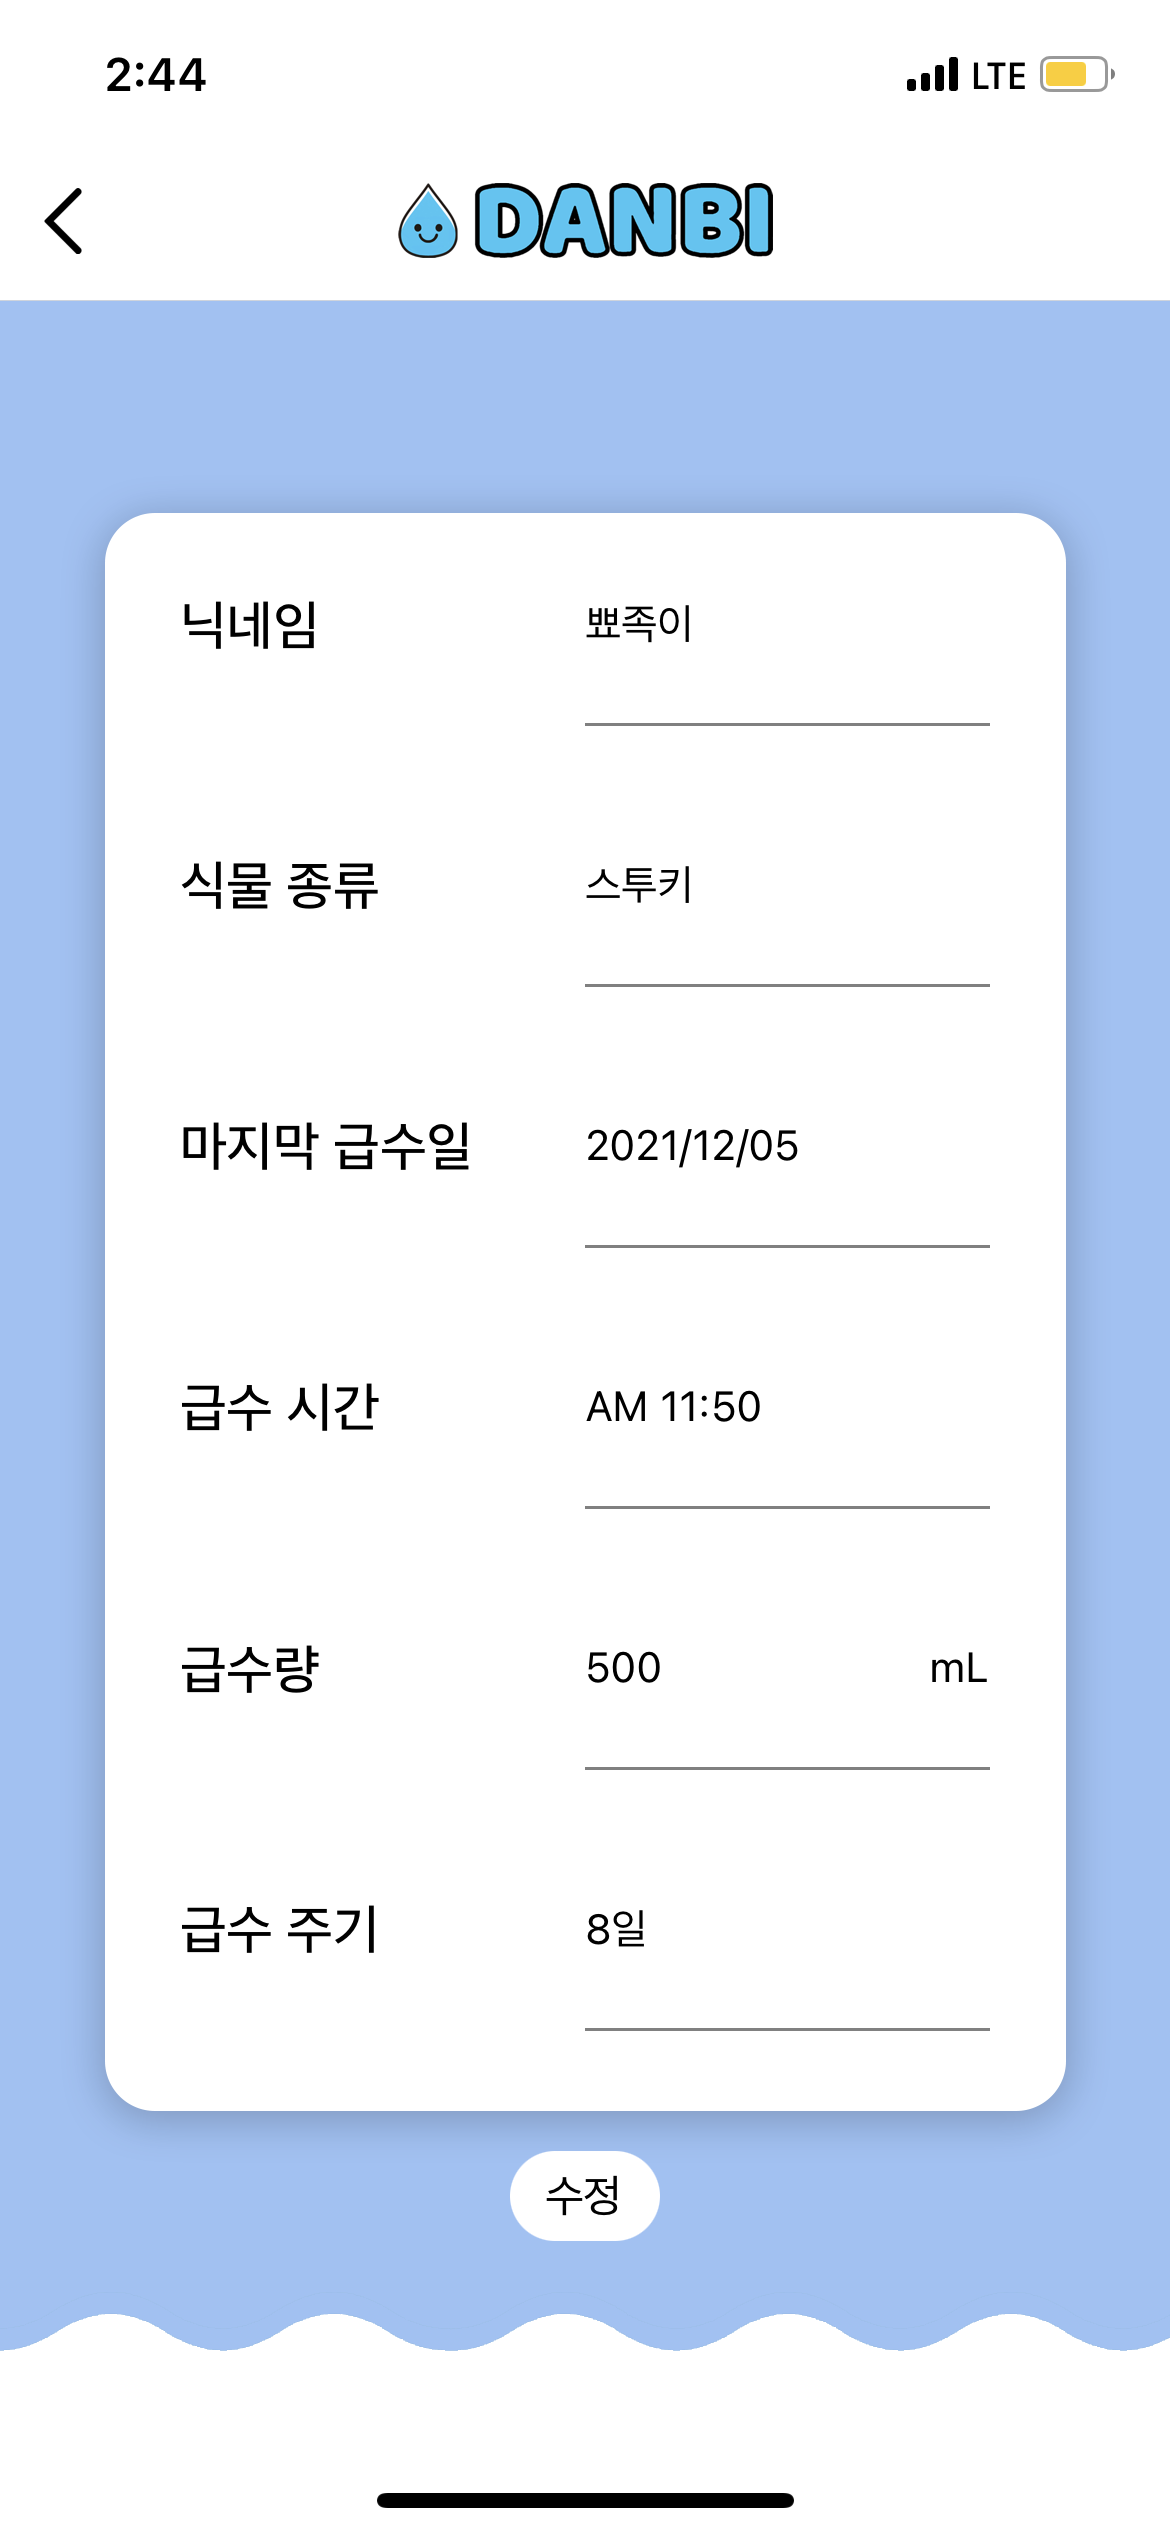
\includegraphics[width=3cm]{page/editPlant.png}
\centering
\caption{Edit\_Plant}
\label{fig:editPlant}
\end{figure}

[Fig. \ref{fig:editPlant}] In the case of plants, the information edit page contains information on Nickname, Plant type, The last water supply date, The water supply time, Water supply amount at once, Water supply cycle. All of these values can also be changed. Among them, when the type is edited, the recommended water supply cycle is provided again, which can be changed by the user.
\item Award Stamp

\par \begin{figure}[h!]
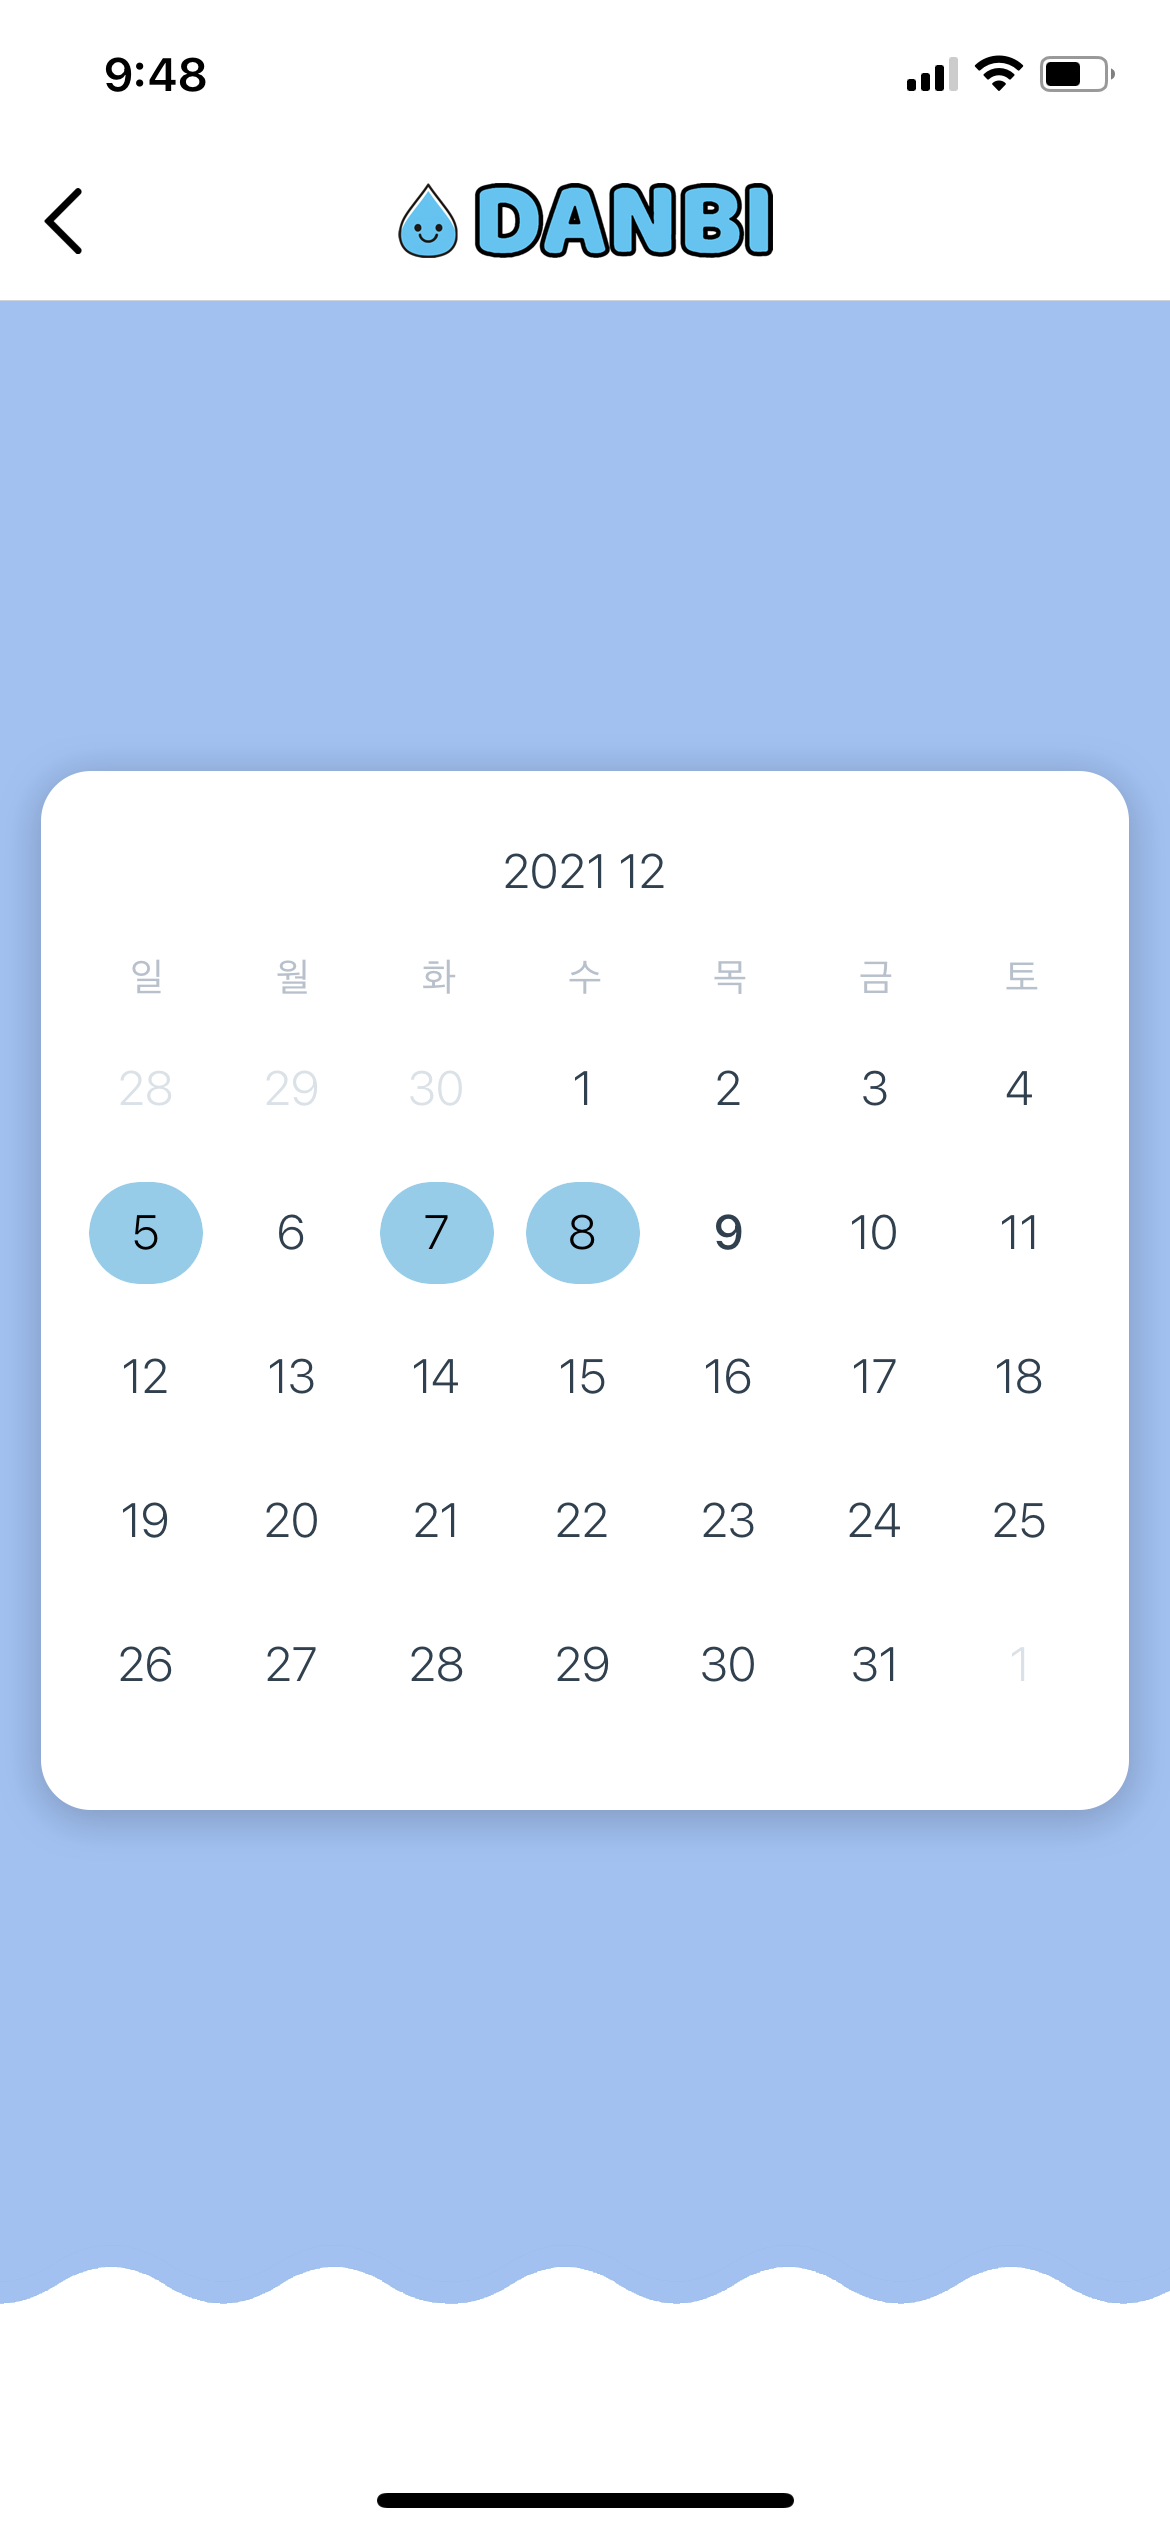
\includegraphics[width=3cm]{page/stamp.png}
\centering
\caption{Stamp calendar}
\label{fig:stamp}
\end{figure}

[Fig. \ref{fig:stamp}] If a user presses the stamp button on the ‘Member specification page’, ‘Award stamp page’ appears and it have a calendar. When the water intake goal is completed, a stamp is stamped on that date. By pressing the triangle button on the left and right sides of the month, it shows the stamps of last and next months. If you press the X mark or select a screen outside the ‘Award stamp page’, the page is turned off.
\end{enumerate}
\item \textbf{Push / Alert Notification}

\par \begin{figure}[h!]
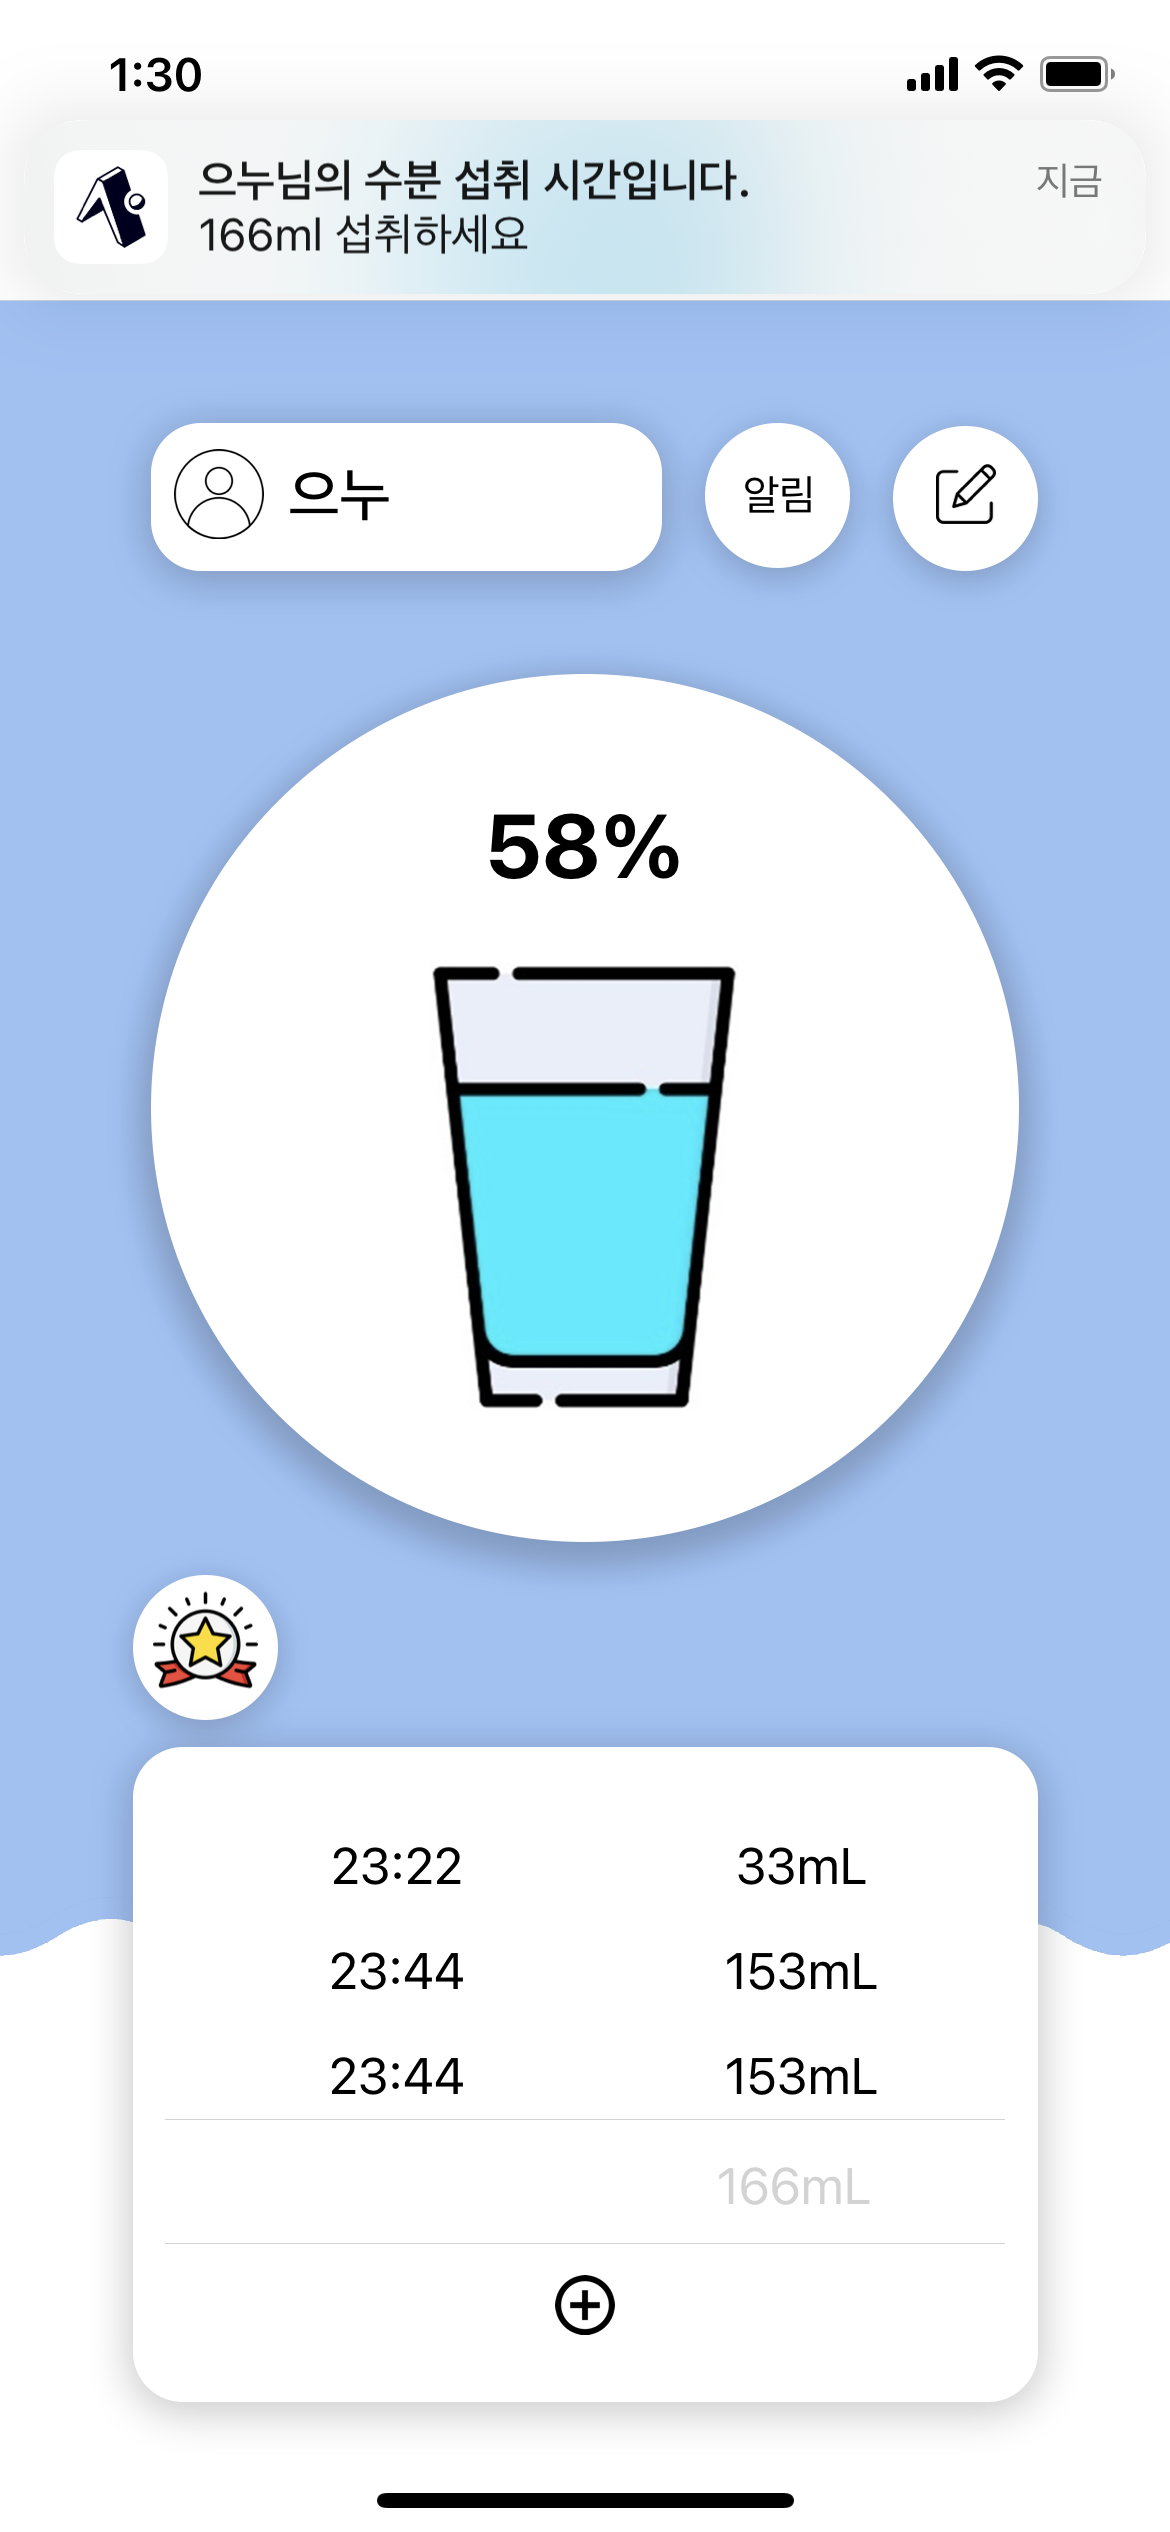
\includegraphics[width=3cm]{page/pushNotification1.png}
\centering
\caption{Push notification 1}
\label{fig:notification1}
\end{figure}

\par \begin{figure}[h!]
\includegraphics[width=3cm]{page/pushNotification2.png}
\centering
\caption{Push notification 2}
\label{fig:notification2}
\end{figure}

\par \begin{figure}[h!]
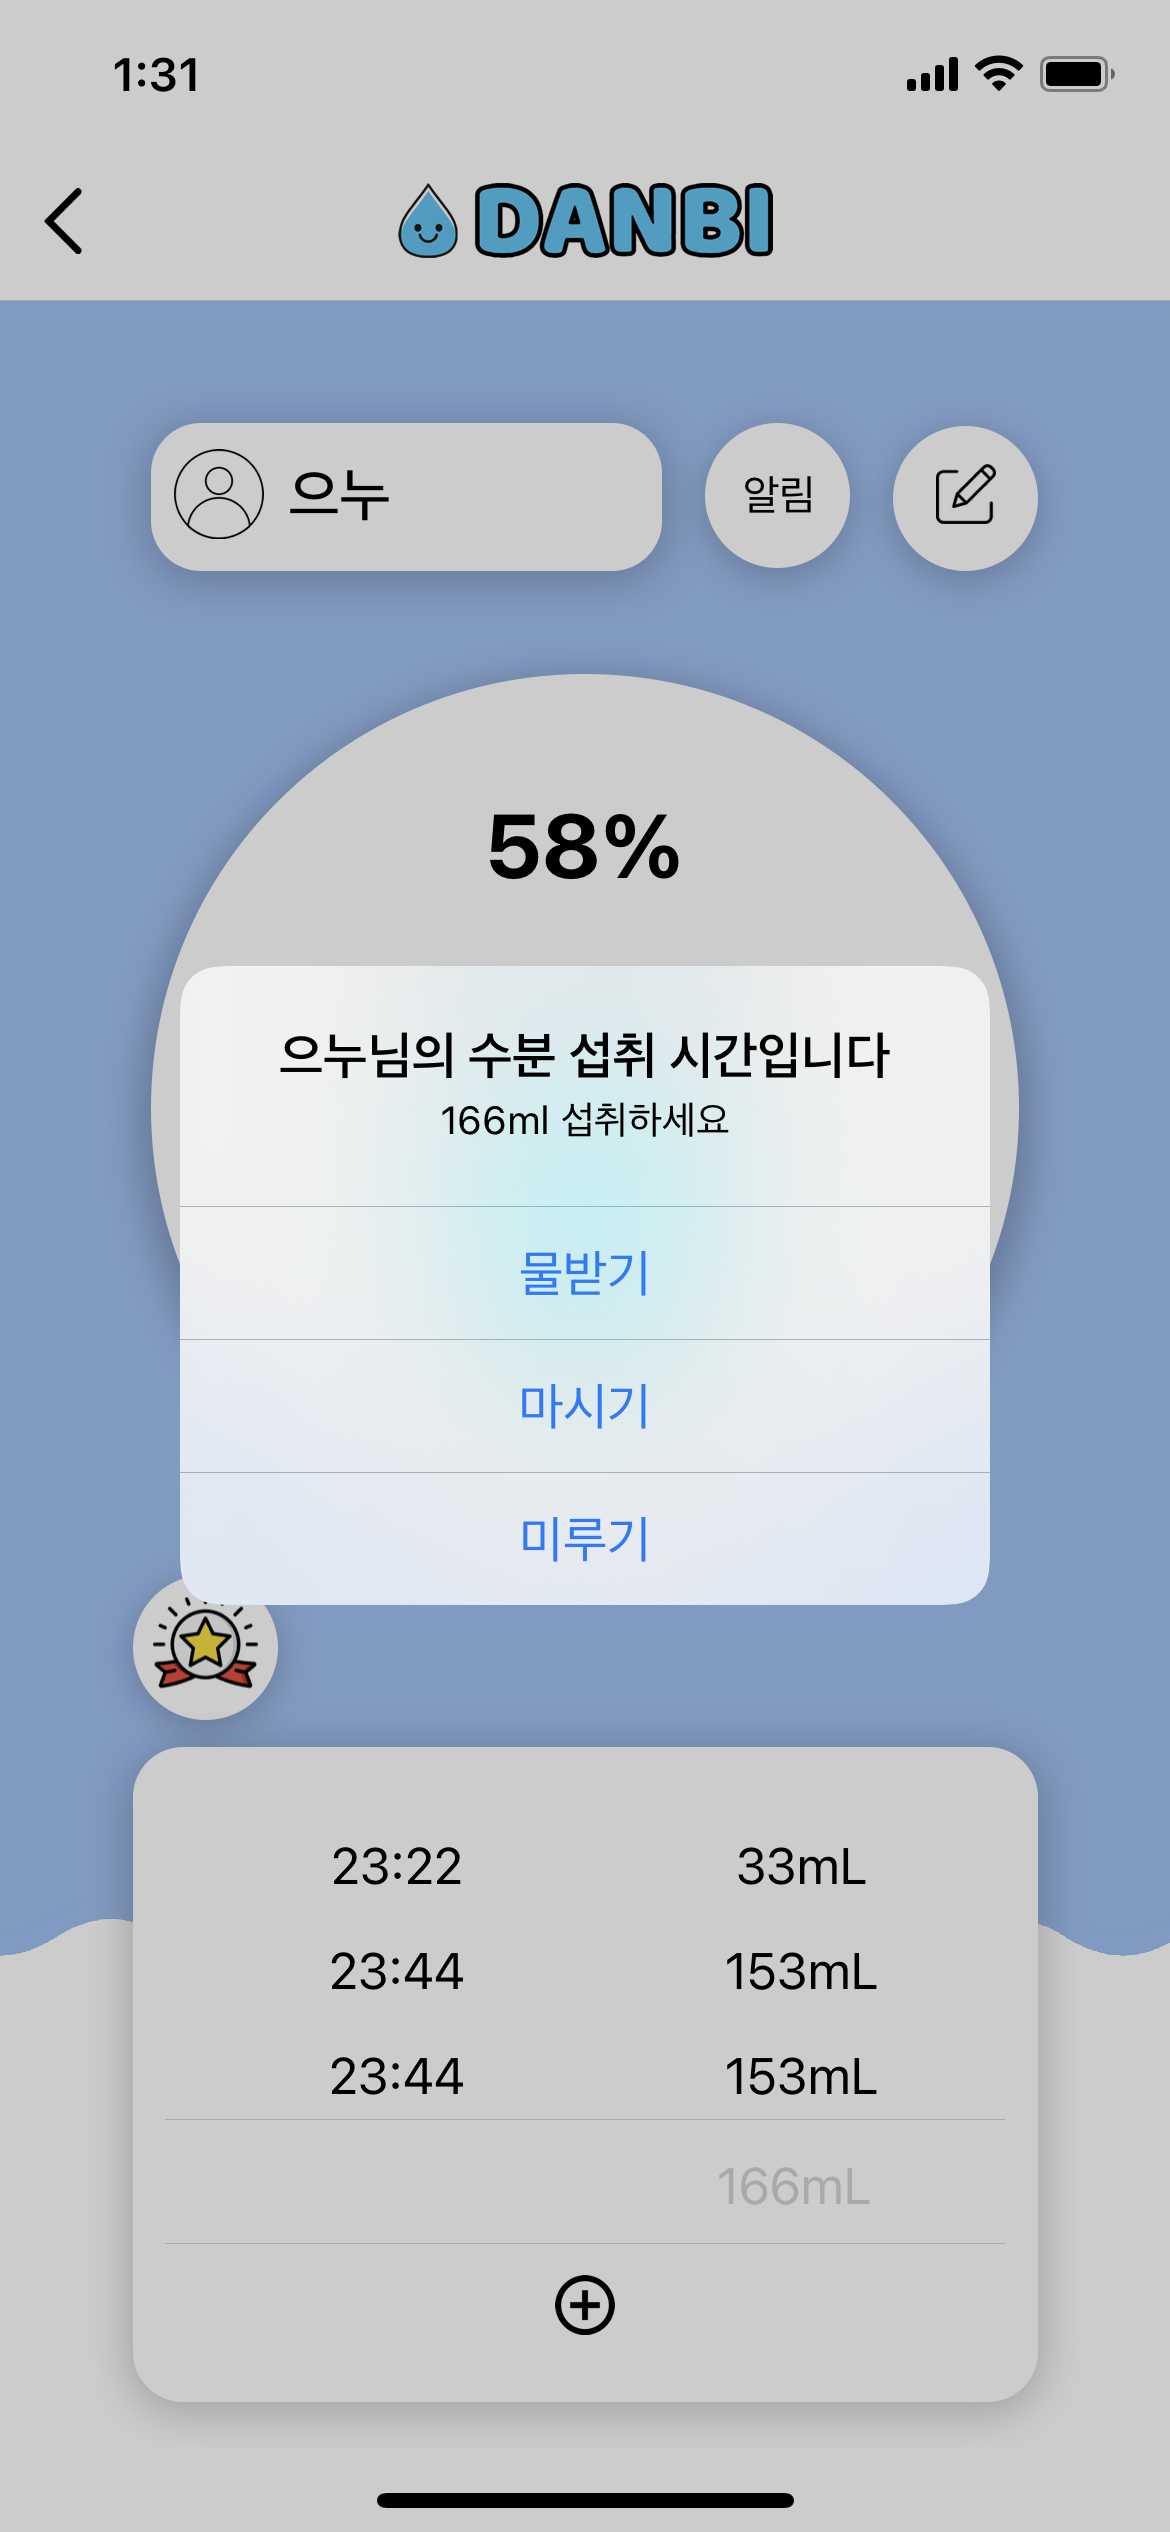
\includegraphics[width=3cm]{page/alert.png}
\centering
\caption{Alert}
\label{fig:alert}
\end{figure}

[Fig. \ref{fig:notification1}] [Fig. \ref{fig:notification2}] When the user's set water intake time comes, a push notification appears on the mobile phone. Touching the push notification leads to an alert notification window [Fig. \ref{fig:alert}] that guides the nickname of members who need to intake water and amount of water intake. Examples are as follows. - "OOO님의 수분 섭취 시간입니다. OOOml 섭취하세요."

There are three buttons that the user can select in the notification. There are ‘물받기’, ‘마시기’, ‘미루기’. The application reacts differently depending on which button the user presses.
\begin{enumerate}
\setlength{\parindent}{2ex}

\par \begin{figure}[h!]
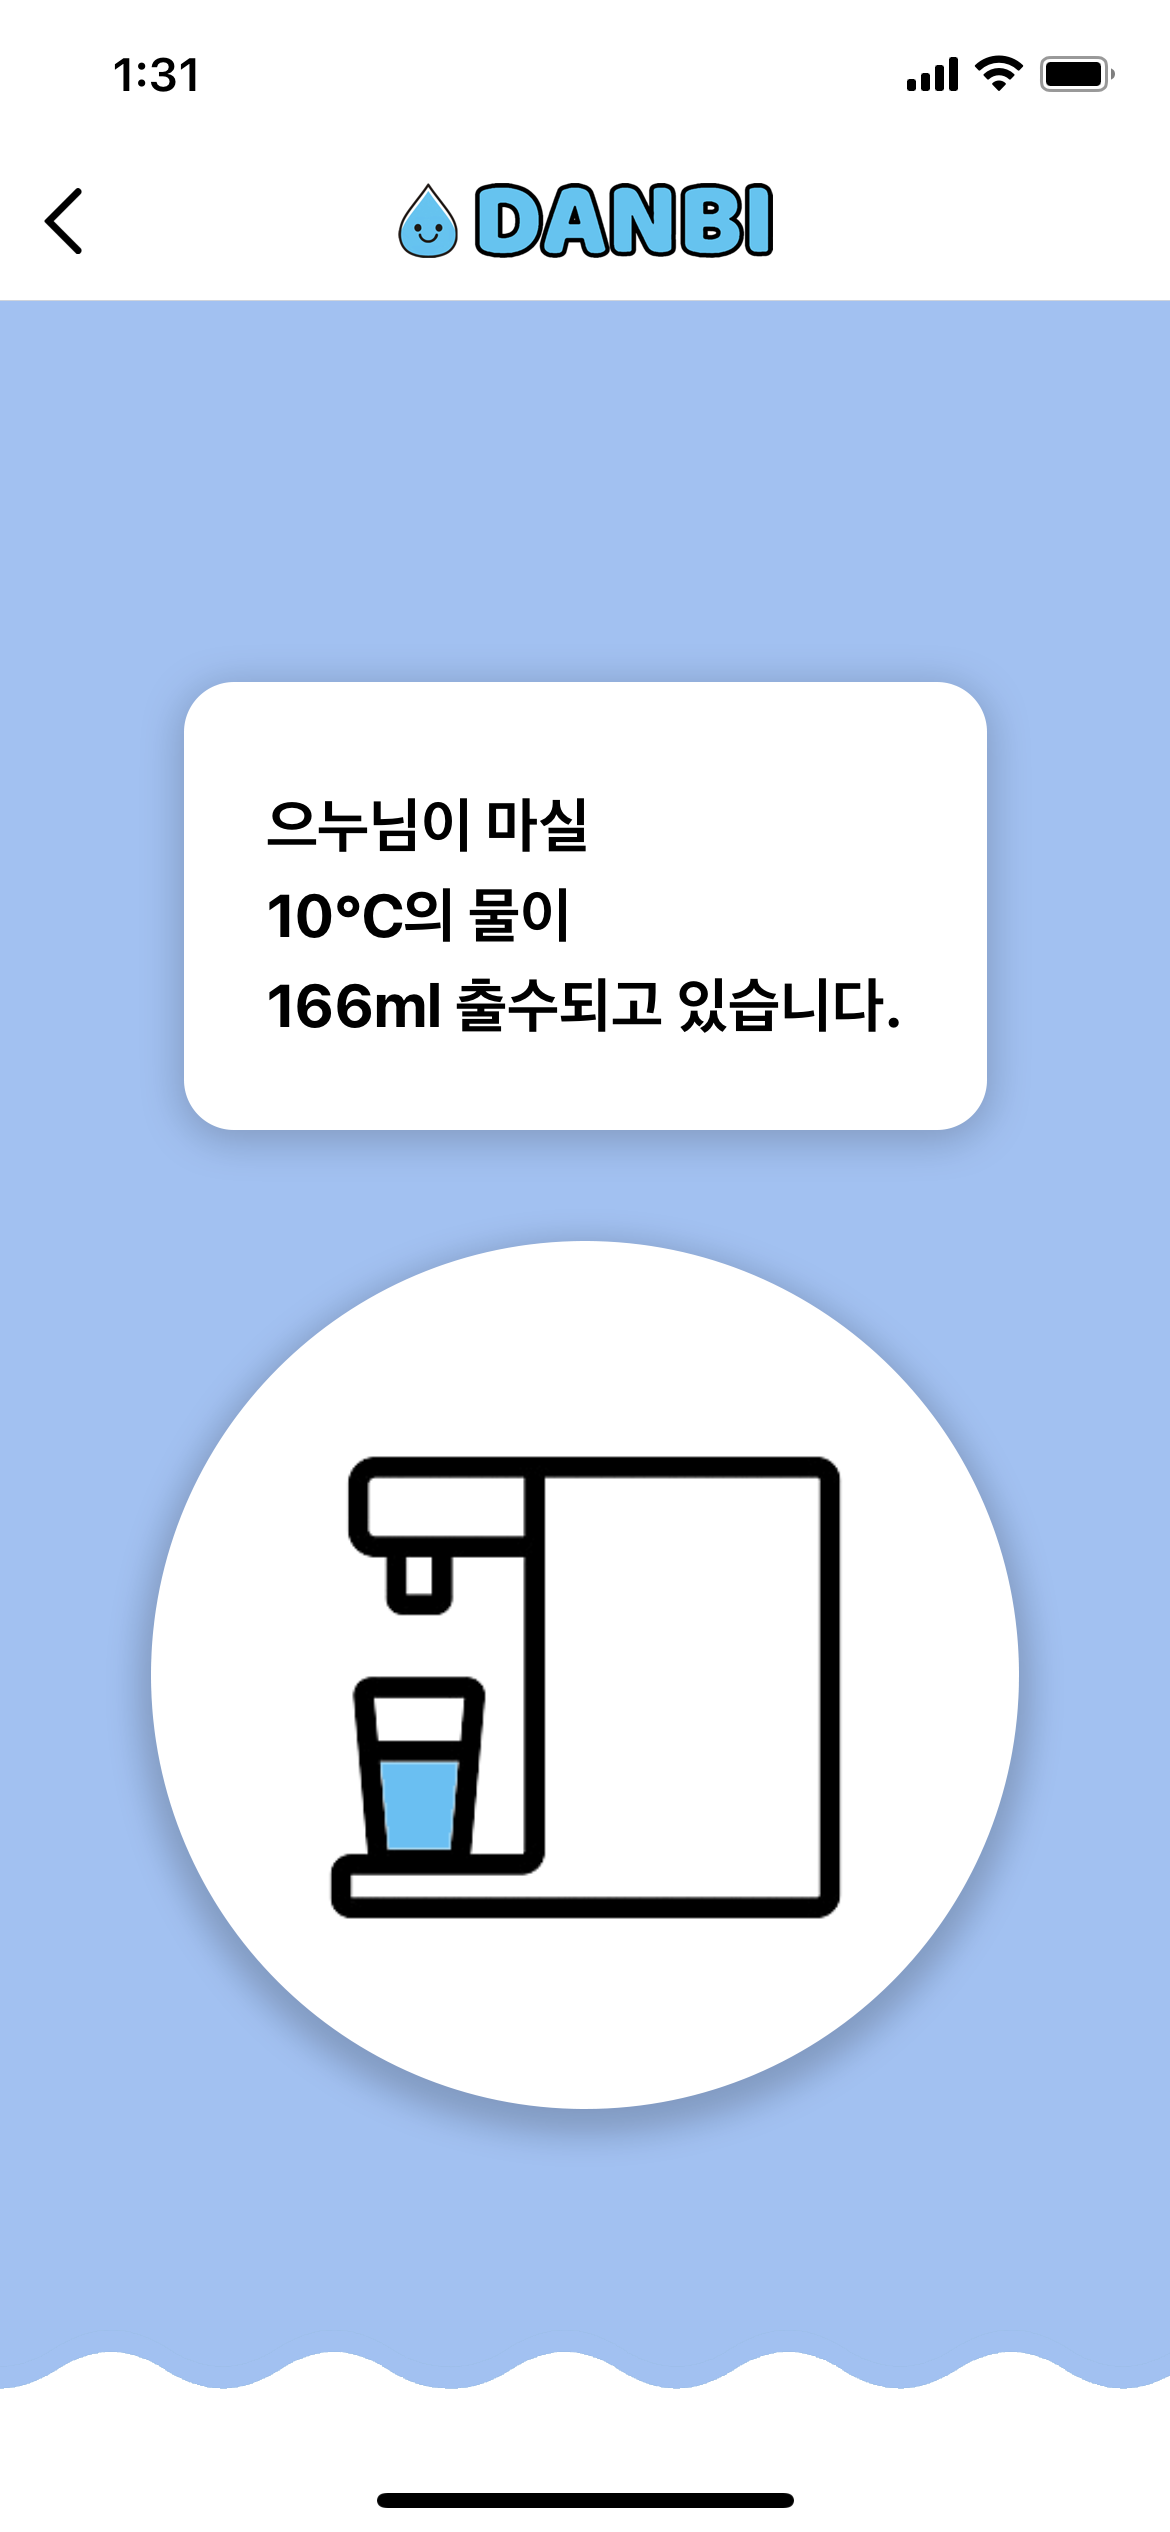
\includegraphics[width=3cm]{page/puricare.png}
\centering
\caption{Puricare}
\label{fig:puricare}
\end{figure}

\item When selecting ‘물받기’, the LG PuriCare water purifier connected to the application offers water according to the amount of water intake at once and water temperature set by the user. [Fig. \ref{fig:puricare}] It also delivers the amount of water intake and the time when the button is pressed to the server, stores it in the database, and updates the application.

\item When selecting '마시기', the amount of water intake and the time when the button is pressed are delivered to the server, stored in the database, and the application is updated.

\item When '미루기' is selected, the application immediately removes the notification and does not update anything.
\end{enumerate}

The notification disappears immediately when the user presses the button on the option. However, after the notification appears for 5 seconds, if the user does not press any button within that time, the application automatically selects ‘미루기’.
\end{itemize}

\subsection{NUGU speaker}
\begin{itemize}
\setlength{\parindent}{2ex}
\setlength{\parskip}{0.5em}
\item \textbf{Notification}

In the same way as the notification of the application, when the water intake time set by the user comes, NUGU speaker notifies the user by voice as follows. - “OOO님의 수분 섭취 시간입니다.”

The reactions that users can make to the notification are '물받기', '마시기', '미루기', which are the same as the reactions in the application. If you want to choose ‘물받기’, you can answer "물 받아줘" to NUGU speakers. If you want to choose ‘마시기’, you can answer "물 마실게" to NUGU speakers. If you want to choose ‘미루기’, you can answer "나중에 마실게" to NUGU speakers. When the user inputs one of the three reactions by voice, the system's response is also the same as in the application. If there is no response from the user for 10 seconds after the notification of the NUGU speaker, '미루기' is automatically selected and DANBI is terminated.

\item \textbf{Communication}

To execute DANBI, the user should say, "단비 켜줘." As the application in NUGU speaker runs, NUGU speaker says, "단비를 실행합니다."

The user can ask three types of questions. There are questions that can check today's water intake, the last time of water intake, and the next time of water intake.

\begin{enumerate}
\setlength{\parindent}{2ex}

\item To check how much water the member intakes today, the user can ask NUGU speaker, “OOO 오늘 물 얼마나 마셨어?” with the nickname of the member that the user wants to check. Then based on the daily water intake stored in the database, NUGU speaker says, “OOO님은 오늘 OOOml(혹은 OL) 마셨습니다. 목표 섭취량까지 OOOml(혹은 O.OL) 남았네요.” If the amount of water is less than 1L, it is guided in ml to deliver the exact value to the user, but if it is more than 1 liter, it is guided in L units to help understand faster. In addition, to prevent the message from getting too long in unit L, it guides upto only one decimal place.

\item The user can ask NUGU speaker when the last water intake time is. If the member you want to check is a human, you can say with the member's nickname, “OOO 언제 물 마셨어?” If a member is a pet or plant, add the member's nickname and say, “OOO 언제 물 줬어?” The NUGU speaker takes the last water intake date and time stored in the database through the server and guides it as follows. In the case of humans and pets, they drink water every day, so along with the time excluding the date, they say, “OOO님의 마지막 수분 섭취 시간은 OO시 (OO분) 입니다.” It guides the time, and if it is at prompt, the notification is concise by omitting how many minutes it is. In addition, if there is no record of water intake yet within a day, it says “OOO님은 아직 오늘의 수분 섭취가 없습니다.” In the case of plants, the interval between water intake is by date, so they say, “OOO님의 마지막 수분 섭취 날짜는 O월 O일입니다.”

\item The user can also ask NUGU speaker when the next water intake time is. If the member you want to check is a person, you can say with the member's nickname, “OOO 언제 물 마셔야 돼?” If a member is an animal or plant, you can add the member's nickname and say, “OOO 언제 물 줘야 돼?" NUGU speaker takes the date and time of water intake from the database through the server and guides it as follows. In the case of humans and animals, they drink water every day, so along with the time excluding the date, they say, “OOO님의 다음 수분 섭취 시간은 OO시 (OO분)입니다.” In addition, if the guidance time is at prompt, minutes are omitted. In the case of plants, the water supply cycle is by date, so along with the date, they say, “OOO님의 다음 수분 섭취 날짜는 O월 O일입니다.”
\end{enumerate}

The notification disappears immediately when the user presses the button on the option. However, after the notification appears for 5 seconds, if the user does not press any button within that time, the application automatically selects ‘미루기’.

\end{itemize}

\subsection{LG PuriCare water purifier}
\setlength{\parindent}{2ex}

When a user selects "물받기" in response to an application notification or NUGU speaker's voice notification, the server sends a query to the LG PuriCare water purifier about the temperature and amount of water set differently for each member. The LG PuriCare water purifier receives the query and automatically offers water according to the set value.

Moreover, through biometric functions such as face recognition and fingerprint recognition of LG PuriCare, the water purifier knows which family member used the water purifier. If a member receives 500ml of water from the water purifier, it recognizes the member and sends the member's name, the amount of water offered, and the time to the DANBI application. Accordingly, the user conveniently records information on water offered from the LG PuriCare water purifier without manually inputting it.

\ 

\section{Architecture Design / Implementation}

\subsection{Overall architecture}\label{AA}
\setlength{\parindent}{2ex}
\par \begin{figure}[h!]
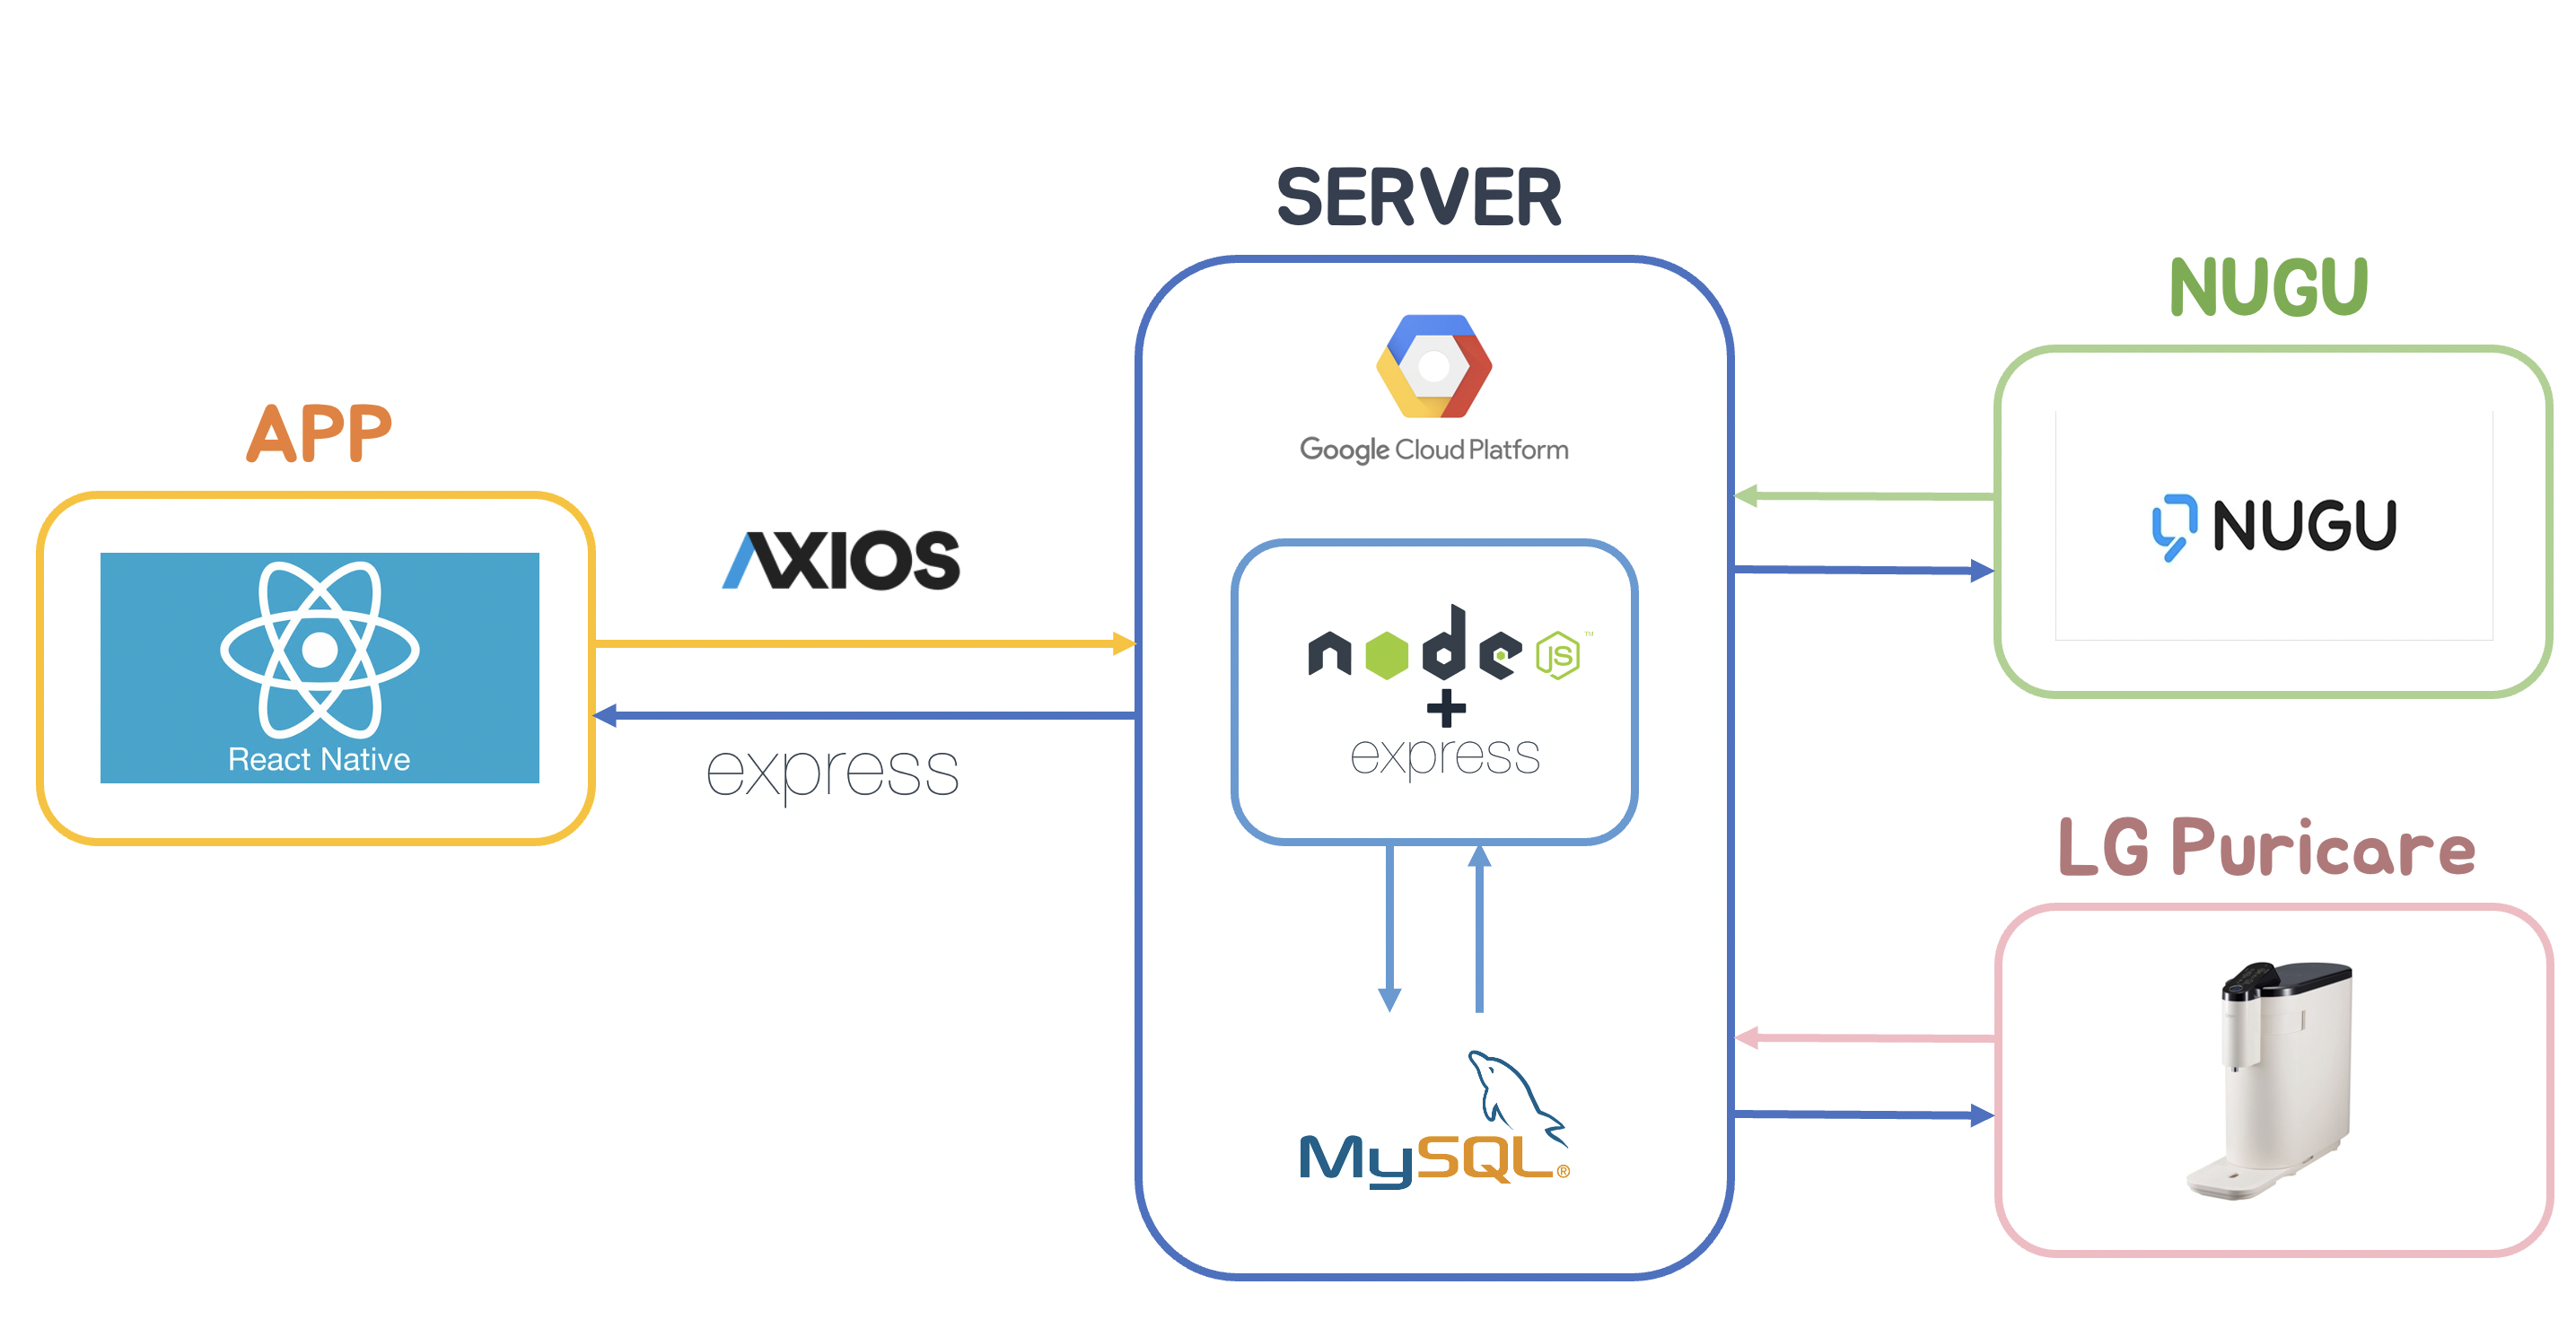
\includegraphics[width=8cm]{image/architecture.png}
\centering
\caption{Overall architecture}
\label{fig:architecture}
\end{figure}

[Fig. \ref{fig:architecture}] DANBI is largely composed of four modules : application, server, NUGU speaker, and LG puricare water purifier. User can use DANBI in two ways, mobile application method and the NUGU speaker method.

The first module is frontend. We designed the application using React Native and JavaScript, and make it possible for the user to use DANBI. The user can check the list of family members that she registered in the DANBI. In addition, the degree of achievement of water intake of each member can be provided as an intuitive picture. In addition, specific water intake time and water intake amount data can be checked. Furthermore, it is possible to check application push notification and can response to this notification, additional member registration, and achievement stamp confirmation.

\par \begin{figure}[h!]
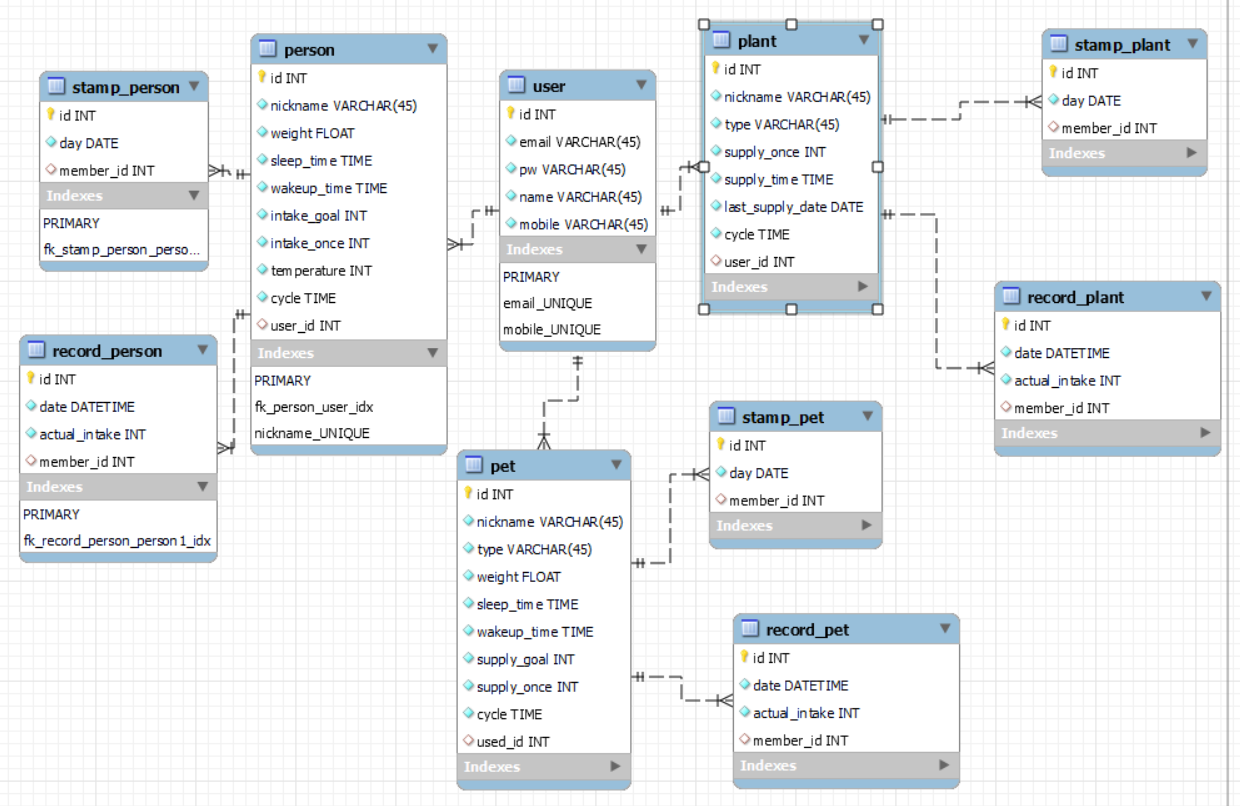
\includegraphics[width=8cm]{image/db.PNG}
\centering
\caption{Database}
\label{fig:db}
\end{figure}

[Fig. \ref{fig:db}] The second module is backend which interacts with the database. We built a backend that delivers information to the frontend using node.js, JavaScript, and express.js. Our database is made by mySQL. Backend receives user account, stores it in database, and manages member information registered by each user account. When the user inputs the member's information, the recommended amount and recommended period of water intake for each member are calculated and the delivered. It also delivers and stores all water intake information of each member to the database. Backend also select and retrieve values that stored in the database so that the user can see the information in the frontend.

The third module is the NUGU playbuilder. It is a service provided by SKT NUGU developers, SKT. We used this to enable users to use the DANBI service by voice. The user can ask the NUGU speaker about each member's water intake information by voice, and the NUGU provides the answer to the user.

\subsection{Directory Organization}
\setlength{\parindent}{2ex}
\begin{table}[h!]

        \begin{threeparttable}
            \caption{Directory Organization - Frontend 1%
            \label{tab:table5}}    %% Caption above tabular, label inside caption
            \begin{tabular}{p{2.4cm}p{2.8cm}p{2cm}}
            \toprule
            \bfseries Directory & \bfseries File name & \multicolumn{1}{l}{\bfseries Modules used} \\
            \midrule
            /DANBI 
            & App.js& react-native-gesture-handler, @react-navigation/stack, react-native, react, @react-navigation/native \\
            & app.json\\
            & package.json\\
            & package-lock.json\\
            \hline
            /DANBI/Source
            & addrecord\_background.png\\
            & back\_btn.png\\
            & background\_test.jpg\\
            & btn\_google.png\\
            & btn\_kakao.png\\
            & btn\_naver.png\\
            & calendadr\_background.png\\
            & cup\_0.png\\
            & cup\_25.png\\
            & cup\_50.png\\
            & cup\_75.png\\
            & cup\_100.png\\
            & DANBI\_Logo.png\\
            & DANBI\_LogoName.png\\
            & DANBI\_Name.png\\
            & edit.png\\
            & entry\_background.png\\
            & login\_background_2\\
            & login\_background\\
            & main\_background\\
            & mytab\_icon\_new.png\\
            & person\_activated.png\\
            & person\_inactivated.png\\
            & pet\_activated.png\\
            & pet\_inactivated.png\\
            & plant\_activated.png\\
            & plant\_inactivated.png\\
            & plus.png\\
            & purifier\_background.png\\
            & purifier.gif\\
            & reg\_background.png\\
            & signup\_background.png\\
            & smallDANBI.png\\
            & spec\_background.png\\
            & stamp.png\\
            & waterIntakePicTest.png\\
            \hline
            /DANBI/screens
            & AddRecord.js& react, react-native, expo-status-bar, react-native-modal-datetime-picker, react-native-picker-select\\
            & ChangePW.js& reat, axios, react-native, react-navigation\\
            & DeleteAccount.js& react-native, react-navigation, react\\
            & Edit\_person.js& react, react-native, expo-status-bar, react-native-modal-datetime-picker, react-native-picker-select\\
        \hline
        /DANBI/node\_modules& ...\\  
            \bottomrule
            \end{tabular}
        \end{threeparttable}
    \end{table}
    
\begin{table}[h!]

\begin{threeparttable}
    \caption{Directory Organization - Frontend 2%
    \label{tab:table5}}    %% Caption above tabular, label inside caption
    \begin{tabular}{p{2.4cm}p{2.8cm}p{2cm}}
    \toprule
    \bfseries Directory & \bfseries File name & \multicolumn{1}{l}{\bfseries Modules used} \\
    \midrule
    /DANBI/screens
     & Edit\_pet.js& react, react-native, expo-status-bar, react-native-modal-datetime-picker, react-native-picker-select\\
            & Edit\_plant.js& react, react-native, expo-status-bar, react-native-modal-datetime-picker, react-native-picker-select\\
            & ForgotId.js& react, react-native, react-navigation\\
            & ForgotPassword.js& react, react-native, react-navigation\\
            & LoginScreen.js& react, react-native, expo-google-app-auth, expo-naver-app-auth, expo-kakao-app-auth, axios\\
            & Logout.js& react, react-native, react-navigation\\
            & Main.js& react, react-native, expo-status-bar, react-navigation\\
             & Purifier.js& react, react-native\\
            & RegistrationScreen.js& react, react-native, @react-navigation/material-top-tabs\\
            & Registration\_person.js& react, react-native, react-native-modal-datetime-picker, react-native-picker-select, axios\\
            & Registration\_pet.js& react, react-native, react-native-modal-datetime-picker, react-native-picker-select, axios\\
            & Registration\_plant.js& react, react-native, react-native-modal-datetime-picker, react-native-picker-select, axios\\
            & Signup.js& react, react-native,@react-navigation/stack, axios\\
    \bottomrule
    \end{tabular}
\end{threeparttable}
\end{table}

\begin{table}[h!]

\begin{threeparttable}
    \caption{Directory Organization - Frontend 3%
    \label{tab:table5}}    %% Caption above tabular, label inside caption
    \begin{tabular}{p{2.4cm}p{2.8cm}p{2cm}}
    \toprule
    \bfseries Directory & \bfseries File name & \multicolumn{1}{l}{\bfseries Modules used} \\
    \midrule
        /DANBI/screens
        & SpecificationScreen.js& react, react-native, expo-notifications, @react-navigation/native, expo-constants, axios\\
        & StampCalendar.js& react, react-native, react-native-calendars\\

    \bottomrule
    \end{tabular}
\end{threeparttable}
\end{table}


\par \begin{figure}[h!]
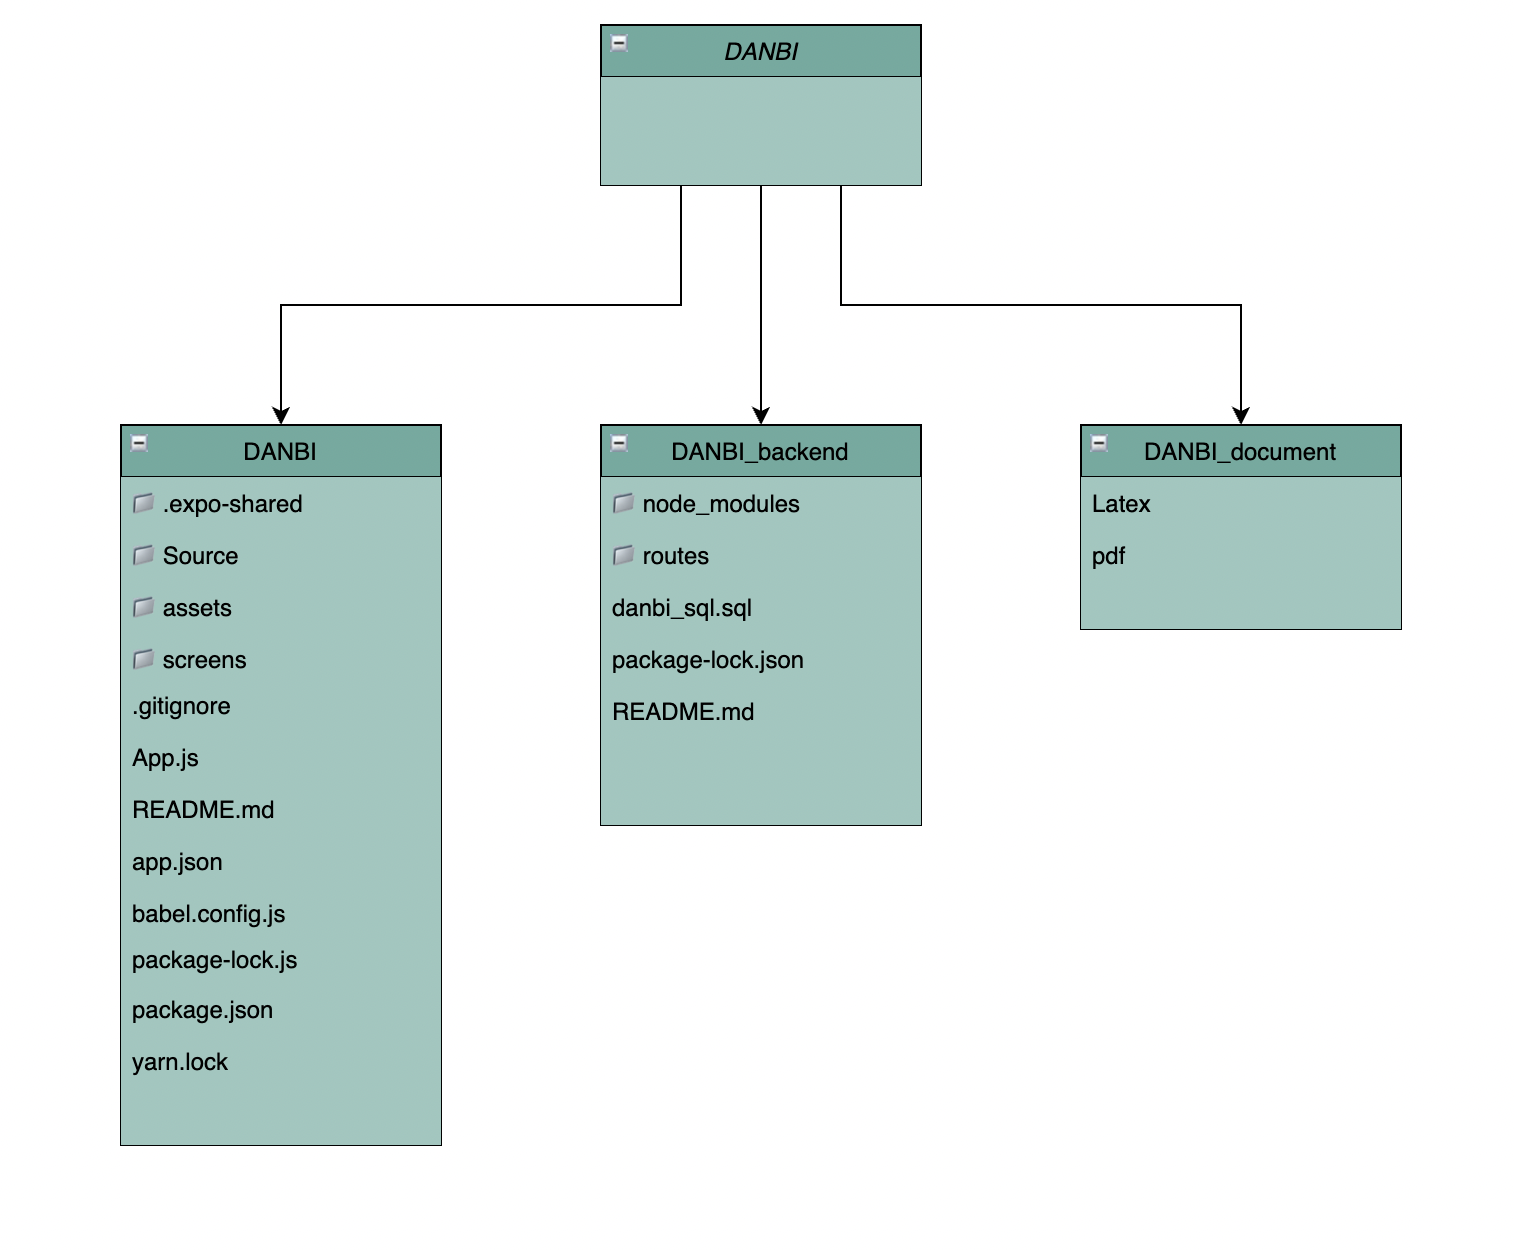
\includegraphics[width=8cm]{image/repo.png}
\centering
\caption{Repository}
\label{fig:repo}
\end{figure}

[Fig. \ref{fig:repo}] DANBI is made up of three github repositories, which is DANBI, DANBI\_backend and DANBI\_document. DANBI repository is about frontend, which has files that related to the overall design and files to interact with the users of DANBI service. Secondly, DANBI\_backend repository has files that work with DANBI repository and database. Also backend repository includes NUGU folder that needed to work with NUGU speaker. The DANBI\_document repository includes Latex and pdf file of the document of our team.

\subsection{Module of Software Component of Class Name}
\setlength{\parindent}{2ex}

\begin{itemize}
    \item Module1 : Frontend
    \begin{enumerate}
    \setlength{\parindent}{2ex}
    \setlength{\parskip}{0.5em}
        \item Purpose
        
        Frontend provides user interface. It serves to connect user and server. It provides an input fields for the user to enter information and deliver the values to the backend. It also provides data in database provided by backend so that the user can see it.
        \item Functionality
        
        Sign up, login, registration of family members(human, animal, plant), reading family member list and show list, reading and show each member's specific water intake information with visual materials, manually input about water intake information, setting notifications, show award stamps. Communicate with server to send the input information from user to database. Show the information that obtained from the database by requesting it to backend.
        
        \ 
        
        \item Location of Source Code
        
        /DANBI
        \item Class Components
        \begin{itemize}
            \item Entry Page
            \setlength{\parindent}{2ex}
            
            It shows DANBI logo during the loading time before the application starts. If the account data is stored on the device, it requests a list of members with the current account data and the screen moves to the Main Page, and if the account data is not stored, it moves to Login Page.
            \item Signup Page
            \setlength{\parindent}{2ex}
            
            It helps users to create an account. It provides input fields for entering name, phone number, email, and password. When the user fills out all the input fields and presses the 'Sign Up' button, the user input value is transferred to the backend to request account creation, and the screen returns to the Login Page. There are Google, Naver, and KakaoTalk buttons are displayed under input fields, and when the user selects the button, frontend requests a social sign-up function to backend according to the selected button.
            \item Login Page
            \setlength{\parindent}{2ex}
            
            It helps users to log in. It provides input fields for entering e-mail and password with the DANBI logo. When the user fills out the input fields and presses the 'Login' button, the user input value is delivered to backend and frontend requests login, and when the login is successfully processed at backend, the list of members registered in the account is delivered to Main page. There are Google, Naver, and KakaoTalk buttons are displayed under the input fields, and when the user selects the button, frontend requests a social login function to backend according to the selected button. At the bottom, 'ID찾기' and '비밀번호찾기'' buttons are displayed so that the user can move to the ForgotId/Forgot password page where account data can be found. In addition, by displaying '회원가입' button, it is possible to move to Signup Page where the user can create an account.
            \item ForgotId / ForgotPassword Page
            \setlength{\parindent}{2ex}
            
            It helps user to find their ID or password. ForgotId Page provides input fields for entering names and phone numbers, and ForgotPassword Page provides input fields for entering name and e-mail. When the user enters all input fields and presses the 'Next' button, the user input value is transferred to backend to check account data and backend provides an ID or password.
            \item ChangePW Page
            \setlength{\parindent}{2ex}
            
            It helps user to change the password of the current account. It provides input fields for entering email, password, and new password. When the user fills all input fields and presses the 'Next' button, the user input value is transferred to backend to change the password. After that, it is logged out and user returns to Login Page.
            \item Main Page
            \setlength{\parindent}{2ex}
            
            It provides a list of members registered in the current account. When a user requests a list of members with the email and password entered by the user, the list of members registered in the current account is received and displayed in the form of a list consisting of images and nicknames when the login is successful. Images provide different images depending on the type of member (person, animal, plant). When a certain member is selected, the screen moves to the Specification Screen Page of the member. The MyTab button is displayed on the upper right side of the screen to provide functions such as changing password, logout, and account deletion.
            \item RegistrationScreen (person, pet, plant) Page
            \setlength{\parindent}{2ex}
            
            It helps user register new family members. Different input fields are provided according to human, pet, and plant so that the user can input biometric information suitable for each type. When the user fills all input fields and presses the '등록' button, the input value is transferred to backend, sends a request for adding members, and moves to the Main Page.
            \item SpecificationScreen Page
            \setlength{\parindent}{2ex}
            
            It provides the member's details to user. When the user requests biometric information with the selected member information to backend, the corresponding information is received to configure an individual Specification Screen Page. A member's name is displayed in the upper left corner, and a button to move to Edit Page to modify the member's biometric information is displayed in the upper right corner. In the center of the screen, the current intake compared to the member's daily target intake is schematically shown in the shape of a water cup. At the bottom, you can see the member's daily water intake record as a list, and at the bottom of the list, there are button that connected to AddRecord Page, where user can add water intake records manually.
            \item AddRecord Page
            \setlength{\parindent}{2ex}
            
            In addition to responding to notification, water intake record can be added manually. It provides an input field that allows user to record of water intake time and amount. When the '등록' button is pressed, the member's water intake information added with the time, and the amount information in the input field are delivered to backend. It requests an additional water intake record and return to the Specification Screen Page.
            \item Edit (person, pet, plant) Page
            \setlength{\parindent}{2ex}
            
            It helps modify existing biometric information. When requesting biometric information along with member information, it brings up an interface suitable for the member type, such as human, animal, and plant. The biometric information of the previously set corresponding member is received from backend, filled and provided in the input field. When the user finishes modifying the information and presses the '수정' button, the user delivers the newly entered biometric information to the backend, requests an information update, and returns to the Specification Screen Page.
            \item StampCalendar Page 
            \setlength{\parindent}{2ex}
            
            It provides a stamped calendar interface on the day that user achieves the water intake goal. When a stamp record is requested to the backend along with the selected member information, the information is provided to the user in the form of receiving it and displaying it on the calendar.
            \item Notification
            \setlength{\parindent}{2ex}
            
            When the water intake time set by the user is reached, the member's name and once water intake amount are sent by the alert. When the currently logged-in account information is delivered to the backend, a notification occurs at the set water intake time of the members registered in the account. In the pop-up notification, the user's response is received by providing '물받기', '마시기', and '미루기' options. The option selected by the user is delivered to the backend so that the backend executes different content that correspond to each option.
        \end{itemize}
        
        \item Where It's taken from
        
        It provides interface that user can see directly. The user enters the information in input field that required to use DANBI service. And also user can show the data which is stored in database with various visual materials.
        \item How / Why you used it
        
        We used React Native with JavaScript. Also we used expo. Through these, we compose pages and made convenient and intuitive UI. These have the advantage of highly productive and easy to build. Expo is especially useful of various reasons. One of them is it support various APIs.
    \end{enumerate}
\end{itemize}

\begin{table}[h!]
        \begin{threeparttable}
            \caption{Directory Organization - Backend%
            \label{tab:table6}}    %% Caption above tabular, label inside caption
            \begin{tabular}{p{2.4cm}p{2.8cm}p{2cm}}
            \toprule
            \bfseries Directory & \bfseries File name & \multicolumn{1}{l}{\bfseries Modules used} \\
            \midrule
            /DANBI\_backend
            & danbi\_sql.sql \\
            & package-lock.json\\
            \hline
            /DANBI\_backend& auth.js & express, mysql\\ 
            /routes &main.js& express, mysql, body-parser, path, cookie-parser, morgan\\
            & member.js& express, mysql\\
            & record.js& express, mysql\\
            & notification.js& express, mysql\\
            & NUGU.js& express, mysql\\
            \hline
            /DANBI\_backend\\
            /node\_modules & ...\\
            \bottomrule
            \end{tabular}
        \end{threeparttable}
    \end{table}

\begin{itemize}
    \item Module2 : Server
    \begin{enumerate}
    \setlength{\parindent}{2ex}
    \setlength{\parskip}{0.5em}
        \item Purpose
        
        The backend server continues to wait for requests from applications and NUGU speaker. When any function calls the server, it manages and responds to the database accordingly. Values are stored and managed in a database.

        The backend server is responsible for bringing whatever data is required from the DB and delivering it from DANBI application made of React Native and NUGU speaker.
        \item Functionality
        
        The server calculates, organizes, and stores information sent from applications and AI speakers in a database. In addition, when an application or AI speaker requests a value, it is taken from the database and returned in addition to the request.
        \item Location of Source Code
        
        /DANBI\_backend
        \item Class Components
        \begin{itemize}
            \item routes/auth
            \setlength{\parindent}{2ex}
            
            It exchanges POST requests and responses to the user's authorization. It can receive necessary information from the user, sign up as a member, and log in through the information the user put in. Afterwards, it is able to delete the account or change the password. If the user forgot ID or password, the user can obtain the information wanted to find through information other than ID and password.
            \item routes/member
            \setlength{\parindent}{2ex}
            
            It contains functions for members assigned to a user. Through registration, users can give different information according to people, animals, and plants and register members. In addition, when a member is selected on the main page, there is a specification POST that hands over information about the member. In addition, it can also enable modification of member information.
            \item routes/record
            \setlength{\parindent}{2ex}
            
            When the user responds to the notification with an application or NUGU speaker, the server receives the request and stores the record in the database. In addition, information is stored when manually inputting or when the water purifier sends the amount of water. In addition, when a member achieves the water intake goal, server receives the date and stores in the database. When the member gets in the stamp calendar, the days of achieving the goal are collected and sent to the application.
            \item routes/notification 
            \setlength{\parindent}{2ex}
            
            The server constantly waits for notification time, and when notification time comes, it delivers information to the application and NUGU speaker about which member have to drink how much water.
            \item routes/NUGU
            \setlength{\parindent}{2ex}
            
            When a user asks a question to a speaker, the server receives what information the speaker needs and what parameters are needed to give the information, and finds the information in the database and sends a response.
            
        \end{itemize}
        
        
        \item Where It's taken from
        
        The backend receives data from the frontend, NUGU speaker, and database.
        \item How / Why you used it
        
        We were able to connect users and databases through the backend server. Users can exchange information through an application, NUGU speaker, or water purifier, and the server plays a role in connecting them all. Since we got used to using JavaScript in React Native, we used node.js for fast development.
    \end{enumerate}
\end{itemize}

\begin{itemize}
    \item Module3 : Database
    \begin{enumerate}
    \setlength{\parindent}{2ex}
    \setlength{\parskip}{0.5em}
        \item Purpose
        
        There is a lot of data in DANBI. There are users, members, records, and stamps, and among them, members are divided into people, animals, and plants. In addition, these information should not be stored inside the mobile phone, but should be provided with login information. We used a database to organize the data well, insert and send appropriate information from time to time.

        Since the information we need is closely related to each other, we used SQL, a relational database, and chose mySQL, which is the most commonly used of them.
        \item Functionality
        
        The server can take information from the outside and put it in the desired table of the database through INSERT. In addition, a user can receive desired information through SELECT, delete data to DELETE, or insert new data from existing data through UPDATE. In addition, data may be conveniently managed through various functions.
        \item Location of Source Code
        
        /DANBI\_backend/danbi\_sql.sql
        \item Class Components
        \begin{itemize}
            \item user
            \setlength{\parindent}{2ex}
            \par \begin{figure}[h!]
            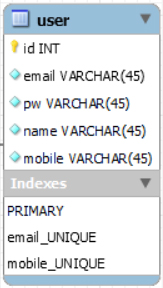
\includegraphics[width=3cm]{image/db_user.jpg}
            \centering
            \caption{User}
            \label{fig:db_user}
            \end{figure}
            
            [Fig. \ref{fig:db_user}] The user table includes index id, email, password, name, and mobile. These four values are essential values for membership. Email is a primary key and allows identification of the user, which is also used to find password. The password is used to log in or delete an account along with an email, and this value may be changed on the password search or password change screen. The name is the user's name and is also used to find password. Phone number is used to find ID.
            \item person
            \setlength{\parindent}{2ex}
            \par \begin{figure}[h!]
            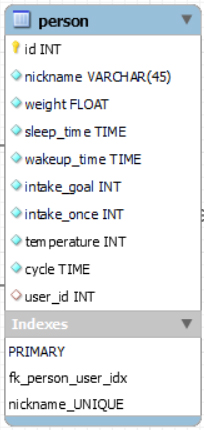
\includegraphics[width=3cm]{image/db_person.jpg}
            \centering
            \caption{Person}
            \label{fig:db_person}
            \end{figure}
            
            [Fig. \ref{fig:db_person}] When a member is a person, information enters this table when the application registers. In the personal table, there are nickname, weight, sleep\_time, wakeup\_time, intake\_goal, take\_once, temperature, and cycle. Nickname is the name of a member, and is displayed on the main screen and the specification screen. Weight is used to calculate intake\_goal. Wakeup\_time, bed\_time, and cycle are used to calculate the notification time and intake\_ounce. Temperature is used to send queries to water purifiers. This table receives the user's id as a foreign key.
            \item pet
            \setlength{\parindent}{2ex}
            \par \begin{figure}[h!]
            \includegraphics[width=3cm]{image/db_pet.jpg}
            \centering
            \caption{Pet}
            \label{fig:db_pet}
            \end{figure}
            
            [Fig. \ref{fig:db_pet}] When a member is a person, information enters this table when the application registers. In the personal table, there are nickname, weight, sleep\_time, wakeup\_time, intake\_goal, take\_once, temperature, and cycle. Nickname is the name of a member, and is displayed on the main screen and the specification screen. Weight is used to calculate intake\_goal. Wakeup\_time, bed\_time, and cycle are used to calculate the notification time and intake\_ounce. Temperature is used to send queries to water purifiers. This table receives the user's id as a foreign key.
            \item plant
            \setlength{\parindent}{2ex}
            \par \begin{figure}[h!]
            \includegraphics[width=3cm]{image/db_plant.jpg}
            \centering
            \caption{Plant}
            \label{fig:db_plant}
            \end{figure}
            
            [Fig. \ref{fig:db_plant}] If the member is a plant, information is entered into this table when registration is performed in the application. Plants do not need sleep\_time or wakeup\_time because the water supply cycle is not time, but date type. Instead, last\_supply\_time was needed to calculate the water supply cycle in date, and supply\_time was required to notify.
            \item record
            \setlength{\parindent}{2ex}
            \par \begin{figure}[h!]
            \includegraphics[width=3cm]{image/db_record.jpg}
            \centering
            \caption{Record}
            \label{fig:db_record}
            \end{figure}
            
            [Fig. \ref{fig:db_record}] Record tables are individually connected to each person, animal, and plant table, but the contents of the column are the same. There is a 'date' column of the DATETIME type, which automatically stores the current time except for manually inputting, and stores the time when manually input is performed. In addition, active\_intake is used to record the amount of water consumed.
            \item stamp
            \setlength{\parindent}{2ex}
            \par \begin{figure}[h!]
            \includegraphics[width=3cm]{image/db_stamp.jpg}
            \centering
            \caption{Stamp}
            \label{fig:db_stamp}
            \end{figure}
            
            [Fig. \ref{fig:db_stamp}] When certain conditions are met, the corresponding members and dates are stored in the stamp. After that, this value is called in the stamp calendar.
        \end{itemize}
        
        \item Where It's taken from
        
        The database receives data from a server.
        \item How / Why you used it
        
        Using the database, we were able to record all the information about users, members, and water intake. It was also possible to get the necessary information through appropriate queries. It was possible to organize the contents to enter the table and draw in detail what information is needed for the DANBI application.
    \end{enumerate}
\end{itemize}

\begin{itemize}
    \item Module4 : NUGU
    \begin{enumerate}
    \setlength{\parindent}{2ex}
    \setlength{\parskip}{0.5em}
        \item Purpose
        
        We use NUGU Play Builder to make user can communicate with  DANBI service through voice. The user can ask about water intake information to NUGU speaker through voice and NUGU speaker provides answer through connect with backend of DANBI.
        \item Functionality
        
        User can ask today's water intake amount of each members, last record of water intake and next schedule of water intake. And NUGU provides information that response to user's request. The notification rings at the set time which informs water intake time and amount. Also it can receive the user's reply and send this reply data to database.
        \item Location of Source Code
        
        /DANBI\_backend/NUGU
        \par \begin{figure}[h!]
        \includegraphics[width=8cm]{image/NUGU.jpg}
        \centering
        \caption{NUGU}
        \label{fig:NUGU}
        \end{figure}
        \item Class Components [Fig. \ref{fig:NUGU}]
        \begin{itemize}
            \item ask.amount 
            \setlength{\parindent}{2ex}
            
            Class of 'ask.amount' determines whether user's question is about the water intake amount by processing predefined entities and intents. The intents used here include {{nickname}} and {{amount}}. If any of the user question's keywords overlap with the {{amount}}, NUGU recognize it as the user asking a question about the amount and link it to the '~/check\_amount' server page to answer it.
            \item ask.record 
            \setlength{\parindent}{2ex}
            
            'ask.record' class determines questions related to record. Record means previous water intake. Intents of {{nickname}} and {{record}} are used to perceive user's questions. If there are {{record}} intent keyword, NUGU recognize it as record asking question. So send request to '~/check\_record' server page.
            \item ask.schedule 
            \setlength{\parindent}{2ex}
            
            Class named 'ask.schedule' examine user's questions about asking water intake schedule. {{nickname}} and {{schedule}} intents are used to determine it. If {{schedule}} intent is included in questions, NUGU perceive it as schedule asking question. And it link to '~/check\_schedule' server page so that it can answer.
            \item check\_amount 
            \setlength{\parindent}{2ex}
            
            'check\_amount' action response to 'ask.amount' request by using database. Specifically, 'actual\_intake' key in DANBI database is correspond to {{amount}} intent, and provide member's today water intake amount by INT value. {{nickname}} intent is used to determine members type of human, animal, plant. Through this process, NUGU provide information that match to user's question as a voice.
            \item check\_record 
            \setlength{\parindent}{2ex}
            
            Class of 'check\_record' is about '~/check\_record' server. This server provide response to 'ask.record' request by using 'date' key in 'record\_person/pet/plant' table in database. This key is correspond to {{record}} intent. So NUGU provide response that put in key to {{record}} which was defined in prompt sentence.
            \item check\_schedule 
            \setlength{\parindent}{2ex}
            
            Class named 'check\_schedule' connected with 'ask.schedule' class. So it provide a response about next water intake schedule of members by using DANBI database. The database values that used to {{schedule}} intent are 'date' and 'cycle'. These two values are calculated in the server and result put in the {{schedule}} intent. So user can provide complete prompt about schedule information through NUGU.
            
        \end{itemize}
        
        \item Where It's taken from
        
        It is taken from backend proxy. And also it is taken from the verbal input by user.
        \item How / Why you used it
        
        We use NUGU Play Builder which is provided by NUGU developers from SKT. We can build play with set Intent, Entity and Action. Intent and Entity are User Utterance Model. Entity is a function that define keywords. With defined keywords, we can define sentences and it is Intent. Action is a function that NUGU provide answers to user. We assigned actions based on database by connect NUGU with backend proxy API, using REST API. We link NUGU speaker to DANBI because it can be more easy for the user. The user may feel  convenient by checking information through voice by NUGU speaker, than handle application.
    \end{enumerate}
\end{itemize}

\begin{itemize}
    \item Module5 : LG Puricare Purifier
    \begin{enumerate}
    \setlength{\parindent}{2ex}
    \setlength{\parskip}{0.5em}
        \item Purpose
        
        Unlike common water purifiers, LG PuriCare water purifier allows users to take water according to the temperature and amount of water they want, and allows them to exchange various information through Wi-Fi. We have not only notified people that they need to drink water or how much they need to drink, but also actually connected to the water purifier to provide more functionality, so that people are not bothered to drink water and can encourage them to drink more regularly.
        
        
        \item Functionality
        
        LG PuriCare water purifier receives data from the server and offers water according to the information. It also identifies members through biometric functions and sends the information to the server to help record intake information.
        
        
        \item Class Components
        \begin{itemize}
            \item offer water
            \setlength{\parindent}{2ex}
            
            When a POST is received from the server, it receives information on the water contained therein and returns the value. In the case of a person, it delivers data of the amount of water and the temperature of water, and in the case of pets and plants, the amount of water and the value of 'purified water'.
            \item member scan
            \setlength{\parindent}{2ex}
            
            Using the biometric function, it identifies who the member is just at that time the member takes water. It delivers information on the water offered along with the member's information and the corresponding time.
        \end{itemize}
        
        \item Where It's taken from
        
        LG PuriCare water purifier receives information on water to offered through the server. In addition, it obtains the member's face information with the face recognition function and member's fingerprint information with the fingerprint recognition function, and can identify the member through comparing them to the existing member's information.
        
        
        \item How / Why you used it
        
        We have made it much more convenient for users to manage water intake through the LG PuriCare water purifier. Smart water purifier that can deliver information through Wi-Fi makes it possible to provide richer functions in DANBI.
        
        
    \end{enumerate}
\end{itemize}

\ 

\section{Use cases [Fig. \ref{fig:usecase}]}

\begin{itemize}
\setlength{\parindent}{2ex}
\setlength{\parskip}{0.5em}
\par \begin{figure}[h!]
\includegraphics[width=8cm]{image/use case.png}
\centering
\caption{Use case}
\label{fig:usecase}
\end{figure}
\item Use Case 1 : Sign-up

User creates an account by entering information of name, phone number, email, and password. User can also use social login services of Google, NAVER, and Kakao. When account register is completed, user is automatically accessed to the login page.
\item Use Case 2 : Login

User can login to DANBI by entering email and password. When the login is completed, user automatically accesses the main page. If the user forgets the email or password, account information can be recovered through each 'ID 찾기' and '비밀번호 찾기' button.
\item Use Case 3 : Logout 

User can login to DANBI by entering email and password. When the login is completed, user automatically accesses the main page. If the user forgets the email or password, account information can be recovered through each 'ID 찾기' and '비밀번호 찾기' button.
\item Use Case 4 : Delete Account

User can delete account of DANBI through the '계정삭제' button in the drawer of the main page. When the account is deleted, all personal information and water intake information of the user are deleted. When the account deletion is completed, user automatically connected to the login page.
\item Use Case 5 : Register Information 

User can register human, animals, and plants as family members. The user can check the information registration form by selecting the entity that she wants to register among the categories of human, animals, and plants in the navigation bar of the information registration page.
\begin{enumerate}
    \item Human: The information required when registering a human member is nickname, weight, wake-up time, sleep time, preferred water temperature, water intake goal, and water intake cycle. Water intake goal is automatically provided based on weight information. The user can freely change this value. After filling out all of the above items and pressing the registration button, the information is stored in the database. Registered information can be modified, and the modified information is updated in the database when the correction completion button is pressed after modifying the desired value.
    \item Pet : The information required when registering a pet member is nickname, type, weight, wake-up time, sleep time, water supply goal, and water supply cycle. Water supply goal is automatically provided based on weight information. The user can freely change this value. After filling out all of the above items and pressing the registration button, the information is stored in the database. Registered information can be modified, and the modified information is updated in the database when the correction completion button is pressed after modifying the desired value.
    \item Plants: Information required when registering plant members includes nickname, plant type, last water supply date, water supply time, water supply amount, and water supply cycle. The water supply cycle is automatically provided based on plant types. The user can freely change this value. If the plant type is set to 'other', the user must directly set the water supply cycle. After filling out all of the above items and pressing the registration button, the information is stored in the database. Registered information can be modified, and the modified information is updated in the database when the correction completion button is pressed after modifying the desired value.
\end{enumerate}
\item Use Case 6 : Communication 

User communicates with the NUGU speaker by voice. When the user says "단비 켜줘", the NUGU speaker is executed. The user may request and receive information on water intake of the family member by NUGU speaker via voice. The specific information on water intake include each member's water intake amount, the remaining water amount until the goal, the date and time of water intake, and the next water intake schedule. User can request these information to NUGU speaker and NUGU provides a response.
\item Use Case 7 : Notification 

Users get notifications which recommend water intake, and react to it. The notifications come through DANBI application or NUGU speaker at the time set by users, and users respond by selecting the button or answering to NUGU speaker. There are three options users can choose, which are '물받기', '마시기' and '미루기'. When the users select '물받기' or '마시기', water intake record will be updated. In the case of '물받기', users can get water set by preferred temperature and amount from LG PuriCare Purifier. If the users select '미루기', the notification will be eliminated without record updating.
\end{itemize}

\ 

\section{Installation Guide}
\setlength{\parindent}{2ex}
\setlength{\parskip}{0.5em}
User can download 'DANBI' on Appstore or Google Playstore.
User can search our application with keywords such as 'DANBI', ’water’,
’water intake’, ’water record', ’단비’, and etc.
When the user presses the ’download’ button, 'DANBI' will be
installed in the user’s cellphone. 'DANBI' can only be used when Wi-Fi or cellular is connected.

\ 

\section{Conclusion}
\setlength{\parindent}{2ex}
\setlength{\parskip}{0.5em}

DANBI is an application that manages water intake, the basis of all life. It is not easy for busy modern people to drink the proper amount of water with the exact water intake cycle. In addition, as the concept of family expands, all family members, including pets and plants, should be responsible for manage water intake. Therefore, we have developed an application DANBI that records the water intake of all family members of humans, pets, and plants and periodically notifies them. Of course, there are many mobile applications on the market that tell you the water intake cycle and the appropriate amount of water intake. However, such applications have to manually fill out the amount of water we drank. For busy modern people, this is very cumbersome, and also it is not easy to determine the exact amount of water intake. In addition, there are no applications on the market that can manage the water intake of people, pets, and plants at once.

DANBI has functions to solve these problems. First of all, water intake from human, pets, and plants can be all managed in DANBI. The convenience of management was provided to user by providing a list of water intake and cycle suitable for each type and allowing them to see our family members list at a glance.

DANBI also has its own advantages. It provides unique functions through linkage with artificial intelligence speaker NUGU and LG's smart water purifier LG Puricare purifier. Notification is received by voice through NUGU speaker, and as it responds by voice, water intake as much as one intake is automatically recorded. In addition, the supply water measured by LG Puricare can be automatically reflected in the water intake record. The application itself is also linked to the water purifier and if user select '물받기' in the water intake notification, the once water intake is discharged from the water purifier, which also automatically records water intake. This automation function will be a great advantage for busy modern people to choose DANBI among several water intake management applications.

Everyone drinks water every day. But the important thing is that very few people drink the right amount of water at the right time. DANBI will become indispensable to the user's day.

All of our team members had no experience developing web or apps, so we had a lot of difficulties during the project. We realized that even the functions we thought were trivial needed a lot of logic and modules, and we could understand how to run the application.

It is thanks to the efforts of all the team members that we, who started the project from the basics of the development language, understanding how to run the application and the server, were able to complete the DANBI in a short time. We will not forget the sense of accomplishment we felt every time we have completed DANBI's function.

Both our application and team members are like welcome rain, DANBI that falls on dry land.

\ 

\begin{thebibliography}{00}
\bibitem{Android1} "Desktop Windows Version Market Share Worldwide". StatCounter Global Stats. Retrieved June 15, 2021.

\bibitem{Android2} "Operating System Market Share Worldwide". StatCounter Global Stats. Retrieved February 11, 2021.

\bibitem{waterIntake_Human} 
\url{http://kwater.or.kr/web/download/info/WRqna.pdf}

\bibitem{waterIntake_Pet}
\url{https://www.notepet.co.kr/news/article/article_view/?idx=17654}

\bibitem{waterIntake_Plant}
\url{https://fuleaf.com/#filter}



\end{thebibliography}

\ 

\thispagestyle{empty}
\listoffigures
\listoftables
\clearpage
\pagenumbering{arabic}




\end{document}
